\documentclass[11pt, oneside]{book}   	% use "amsart" instead of "article" for AMSLaTeX format
% !TEX encoding = UTF-8 Unicode
\usepackage[french,english]{babel}
\usepackage[T1]{fontenc}
\usepackage[utf8]{inputenc}


\usepackage[]{geometry} 

\usepackage{graphicx}
\setkeys{Gin}{width=\linewidth,totalheight=\textheight,keepaspectratio}
\graphicspath{{graphics/}}
\usepackage[export]{adjustbox}
	
\usepackage{amssymb}
\usepackage{tabularx}
\usepackage{mdwlist}
\usepackage{float}
\usepackage{placeins} % float barriers

\usepackage{pdfpages}

\usepackage{hyperref}
\hypersetup{
	colorlinks = true,
	urlcolor = cyan
}

\usepackage{fancyvrb}
\fvset{fontsize=\normalsize}

\DefineVerbatimEnvironment{VerbatimText}{Verbatim}{frame=lines,framesep=2mm,numbers=left,numbersep=3mm}
\DefineVerbatimEnvironment{VerbatimRaw}{Verbatim}{frame=lines,framesep=2mm}
\DefineVerbatimEnvironment{VerbatimErl}{Verbatim}{frame=lines,framesep=2mm,fontsize=\small}
\DefineVerbatimEnvironment{VerbatimEshell}{Verbatim}{frame=lines,framesep=2mm,fontsize=\small}

\newcommand{\filename}[1]{\Verb`#1`}
\newcommand{\app}[1]{\Verb`#1`}
\newcommand{\otpapp}[1]{\Verb`#1`}
\newcommand{\module}[1]{\Verb`#1`}
\newcommand{\function}[1]{\Verb`#1`}
\newcommand{\expression}[1]{\Verb`#1`}
\newcommand{\command}[1]{\Verb`#1`}
\newcommand{\var}[1]{\Verb`#1`}
\newcommand{\term}[1]{\Verb`#1`}


%% Colors of footnotes
\renewcommand\thefootnote{\textcolor{violet}{\arabic{footnote}}}
%% Colors of figure refs for table of contents and list of figures
\hypersetup{linkcolor=black}

\def\includecode{\begingroup
\catcode`\_=12
\includecodeB}
\newcommand{\includecodeB}[2][erlang]{\VerbatimInput[frame=lines,framesep=2mm,%label=#1/#2,
fontsize=\small]{#1/#2}\endgroup}

%%% Cover

%\title{Stuff Goes Bad:\protect\\ Erlang in Anger}
%\author{
\includegraphics[width=150pt]{heroku-logo-light.pdf}\\
%Fred Hébert}

%\date{}							% Activate to display a given date or no date

\begin{document}
%\maketitle

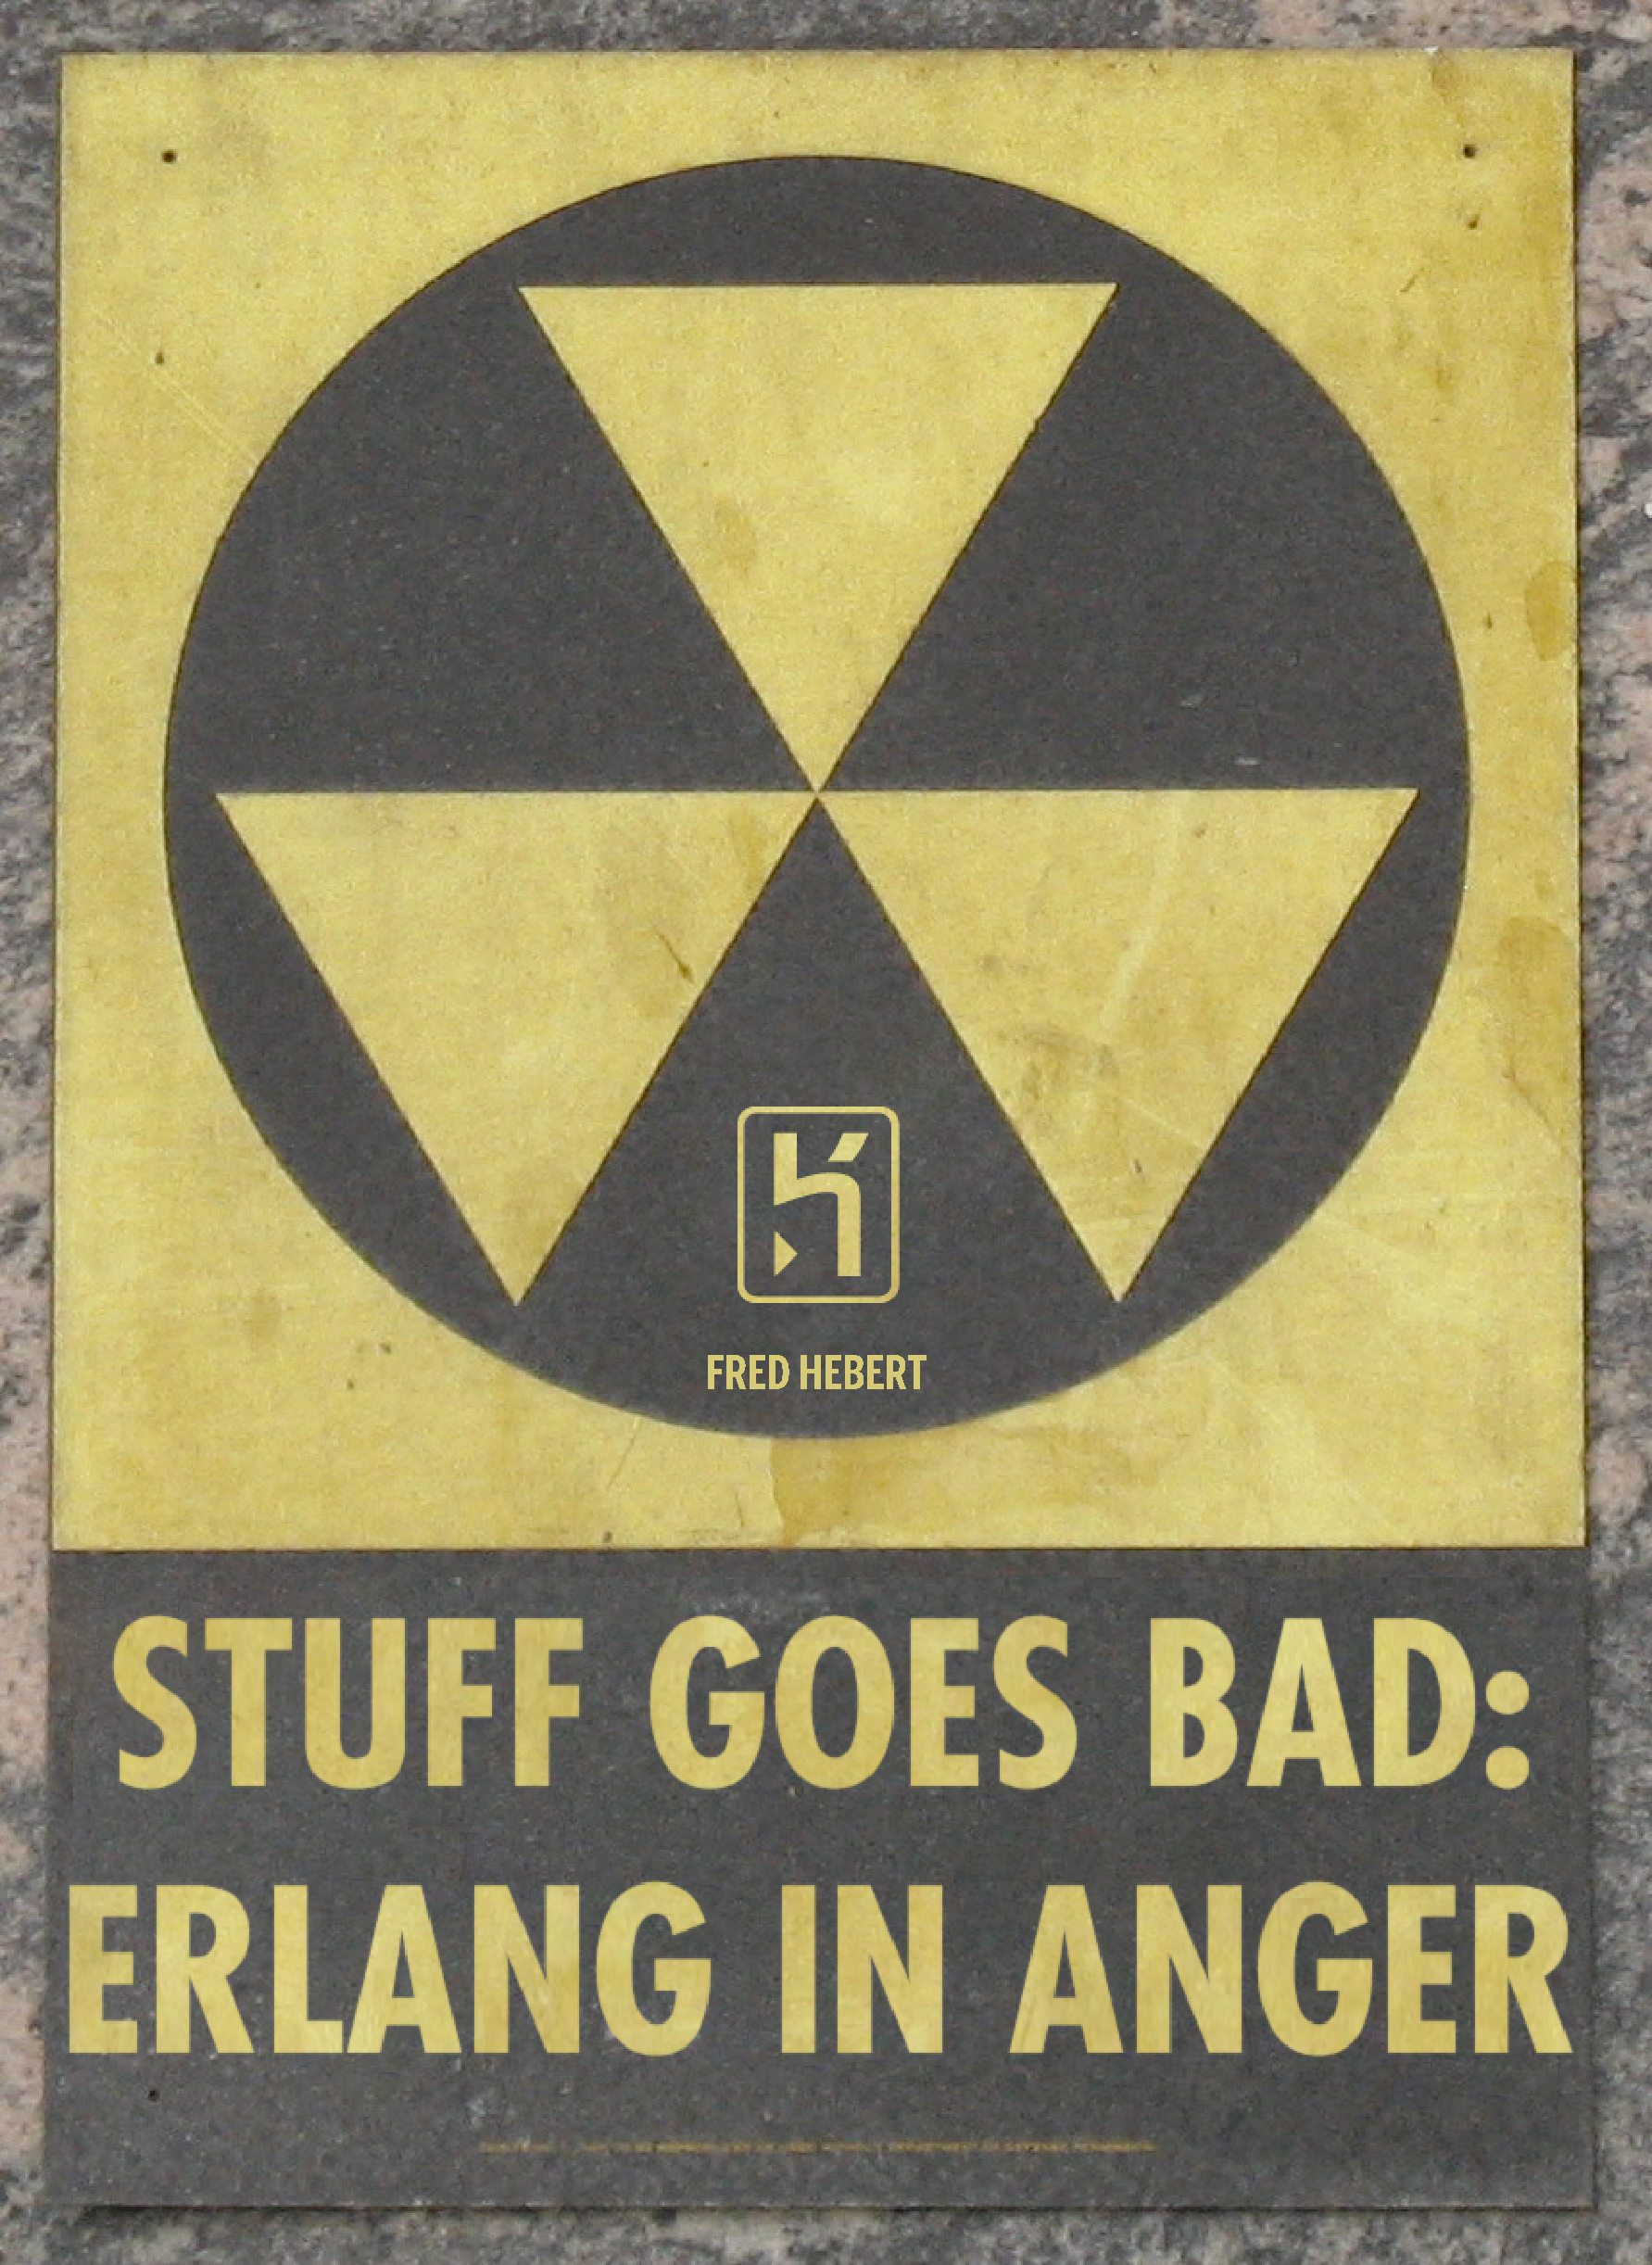
\includepdf[fitpaper=true]{graphics/cover.pdf}

%%% Copyright page
\clearpage
\thispagestyle{empty}
\vspace*{\fill}



\begin{center}
\includegraphics[width=100pt]{by-nc-sa.eps}
\end{center}

\begin{center}
\emph{Stuff Goes Bad: Erlang in Anger} by Fred Hébert and Heroku is licensed under a \href{http://creativecommons.org/licenses/by-nc-sa/4.0/}{Creative Commons Attribution-NonCommercial-ShareAlike 4.0 International License}.
\end{center}

Thanks for the additional work, reviewing, and/or editing done by:

\emph{Jacob Vorreuter}, \emph{Seth Falcon}, \emph{Raoul Duke}, \emph{Nathaniel Waisbrot}, ...

\null
\vfill
%\vspace*{\fill}

The cover image is a modified version of from \href{http://www.freeimages.com/photo/533163}{fallout shelter} by \href{http://www.freeimages.com/profile/drouu}{drouu} on \href{http://sxc.hu}{sxc.hu}.

%% License as of Monday, August 18, 2014:
%%
%% you may use any of my photos, original or modified, for any purpose whatsoever (personal, non-profit, or commercial; for web or print). you do not need to contact me prior to or after using one of my photos, though a comment or note is always appreciated if you have the opportunity.
%%
%% you may not claim ownership or copyright of my photos. seriously, i have an orbital karma gun and i'm not afraid to use it.

\clearpage
%%%


\tableofcontents

\listoffigures

%% Colors of figure refs for text
\hypersetup{linkcolor=violet}


\chapter{Introduction}
\label{chap:introduction}

\section{On Running Software}
\label{sec:on-running-software}

There's something rather unique in Erlang in how it approaches failure compared to most other languages out there. In general, there's this kind of standard way of thinking where the language, programming environment, and methodology do everything possible to prevent errors. Something going wrong at run-time is something that needs to be prevented, and if it cannot be prevented, then it's out of scope for whatever solution people have been thinking about.

The program is written once, and after that, it's off to production, whatever may happen there. If there are errors, new versions will need to be shipped.

Erlang, on the other hand, takes the approach that failures will happen no matter what, whether they're developer, operator, or hardware related. It is rarely practical or even possible to get rid of all errors in a program or a system.\footnote{life-critical systems are usually excluded from this category, but some cases still happen.} If you can deal with some errors rather than preventing them at all cost, then most undefined behaviours of a program can go in that "deal with it" approach.

This is where the "Let it Crash"\footnote{Erlang people now seem to favour "let it fail", given it makes people far less nervous.} idea comes from: Because you can now deal with failure, and because the cost of weeding out all of the complex bugs from a system before it hits production is often prohibitive, the programmer should only deal with the errors he or she knows how to handle, and leave the rest for another process (a supervisor) or the virtual machine to deal with.

Given that most bugs are transient\footnote{131 out 132 bugs are transient bugs (they're caused by circumstances, and trying again may solve the problem entirely), according to Jim Gray in \href{http://www.hpl.hp.com/techreports/tandem/TR-85.7.html}{Why Do Computers Stop and What Can Be Done About It?}}, simply restarting processes back to a state known to be stable when encountering an error can be a surprisingly good strategy.

Erlang is a programming environment where what you have is equivalent to the human body's immune system, whereas most other languages only care about hygiene to make sure no germ enters the body. Both forms appear extremely important to me. Pretty much every environment offers the hygiene, to varying degrees. Nearly no other environment offers the immune system where errors at run time can be dealt with and seen as survivable.

Because the system doesn't collapse the first time something bad touches it, Erlang/OTP also allows you to be a doctor. You can go in the system, pry it open, carefully observe everything inside as it runs, and even try to fix it interactively. To continue with the analogy, Erlang allows you to perform extensive tests to diagnose the problem and various degrees of surgery (even very invasive surgery), without the patient needing to sit down or interrupt his daily activities.

This book intends to be a little guide about how to be the Erlang medic in a time of war. It is first and foremost a collection of tips and tricks to help understand where failures come from, and a dictionary of different code snippets and practices that helped developers debug production systems that were built in Erlang.

\section{Who is this for?}
\label{sec:who-is-this-for}

This book is not for beginners. There is a gap left between most tutorials, books, training sessions, and actually being able to operate, diagnose, and debug running systems once they've made it to production. There's a fumbling phase implicit to a programmer's learning of a new language and environment, where you just have to figure how to get out of the guidelines and step into the real world, with the community that goes with it.

This book assumes that the reader is proficient in basic Erlang and the OTP framework. Erlang/OTP features are explained as I see fit — usually when I consider them tricky — and it is expected that a reader who feels confused by usual Erlang/OTP material will have an idea of where to look for explanations if necessary\footnote{I do recommend visiting \href{http://learnyousomeerlang.com}{Learn You Some Erlang} or the regular \href{http://www.erlang.org/erldoc}{Erlang Documentation} if a free resource is required}.

What is not assumed is that the reader necessarily knows how to debug Erlang software, dive into an existing code base, diagnose issues, or has an idea of some of the best practices about deploying Erlang in a production environment\footnote{Running Erlang in a screen or tmux session is \emph{not} a deployment strategy.}.

\section{How To Read This Book}
\label{sec:how-to-read-this-book}

The book is divided in two parts. 

Part \ref{part:writing-applications} focuses on how to write applications. It includes how to dive into a code base (Chapter \ref{chap:how-to-dive-into-a-code-base}), how most open source Erlang software is written (Chapter \ref{chap:building-open-source-erlang-software}), and how to plan for overload in your system design (Chapter \ref{chap:overload}).

Part \ref{part:diagnosing-applictions} focuses on being an Erlang medic and concerns existing, living systems. It contains instructions on how to connect to a running node (Chapter \ref{chap:connecting}), and the basic runtime metrics you should plan to make visible and are available to you (Chapter \ref{chap:runtime-metrics}). It also explains how to do the autopsy of a system using a crash dump (Chapter \ref{chap:crash-dumps}), how to identify and solve memory leaks (Chapter \ref{chap:memory-leaks}) and how to find what is using up all your CPU (Chapter \ref{chap:cpu-hogs}). The final chapter contains instructions on how to trace Erlang function calls in production using \otpapp{recon}\footnote{\href{http://ferd.github.io/recon/}{http://ferd.github.io/recon/} — a library used to make the text lighter, and with generally production-safe functions.} to understand issues before they bring the system down (Chapter \ref{chap:tracing}).

Each chapter is followed up by a few optional exercises in the form of questions or hands-on things to try if you feel like making sure you understood everything, or if you want to push things further.
%%%
%%%
%%%

\part{Writing Applications}
\label{part:writing-applications}

\chapter{How to Dive into a Code Base}
\label{chap:how-to-dive-into-a-code-base}

"Read the source" is one of the most annoying things to be told, but dealing with Erlang programmers, you'll have to do it often. Either the documentation for a library will be incomplete, outdated, or just not there. In other cases, Erlang programmers are a bit similar to Lispers in that they will tend to write libraries that will solve their problems, and not really test or try them in other circumstances, leaving it to you to extend or fix issues that arise in new contexts.

It's thus pretty much guaranteed you'll have to go dive in some code base you know nothing about, either because you inherited it at work, or because you need to fix it or understand it to be able to move forward with your own system. This is in fact true of most languages whenever the project you work on is not one you architected yourself.

There are three main types of Erlang code bases you'll encounter in the wild: raw Erlang code bases, OTP applications, and OTP releases. In this chapter, we'll look at each of these and try to provide helpful tips on navigating them.

\section{Raw Erlang}
\label{sec:dive-raw-erlang}

If you encounter a raw Erlang code base, you're pretty much on your own. These rarely follow any specific standard, and you have to dive in the old way to figure out whatever happens in there.

This means hoping for a \filename{README.md} file or something similar that can point to an entry point in the application, and going from there, or hoping for some contact information that can be used to ask questions to the author(s) of the library.

Fortunately, you should rarely encounter raw Erlang in the wild, and they are often beginner projects, or awesome projects that were once built by Erlang beginners and now need a serious rewrite. In general, the advent of tools such as \app{rebar}\footnote{\href{https://github.com/rebar/rebar/}{https://github.com/rebar/rebar/} — a build tool briefly introduced in Chapter \ref{chap:building-open-source-erlang-software}} made it so most people use OTP Applications, even when releases would be appropriate.\footnote{See Section \ref{sec:dive-otp-releases}}

\section{OTP Applications}
\label{sec:dive-otp-applications}

Figuring out OTP applications is usually rather simple. They usually all share a directory structure that looks like:

\begin{VerbatimRaw}
doc/
ebin/
src/
test/
LICENSE.txt
README.md
rebar.config
\end{VerbatimRaw}

There might be slight differences, but the general structure will be the same.

Each OTP application should contain an \emph{app file}, either \filename{ebin/<AppName>.app} or more often, \filename{src/<AppName>.app.src}\footnote{a build system generates the final file that goes in \filename{ebin}. Note that in these cases, many  \filename{src/<AppName>.app.src} files do not specify modules and let the build system take care of it.}. There are two main varieties of app files:

\includecode[erlang]{useragent.app.src}

And:

\includecode[erlang]{dispcount.app}

This first case is called a \emph{library application}, while the second case is a regular \emph{application}.

\subsection{Library Applications}
\label{subsec:dive-library-applications}

Library applications will usually have modules named \module{\emph{appname}\_something}, and one module named \module{\emph{appname}}. This will usually be the interface module that's central to the library and contains a quick way into most of the functionality provided.

By looking at the source of the module, you can figure out how it works with little effort: If the module adheres to any given behaviour (\module{gen\_server}, \module{gen\_fsm}, etc.), you're most likely expected to start a process under one of your own supervisors and call it that way. If no behaviour is included, then you probably have a functional, stateless library on your hands. For this case, the module's exported functions should give you a quick way to understand its purpose.

\subsection{Regular Applications}
\label{subsec:dive-regular-applications}

For a regular OTP application, there are two potential modules that act as the entry point:

\begin{enumerate*}
	\item \module{\emph{appname}}
	\item \module{\emph{appname}\_app}
\end{enumerate*}

The first file should be similar in use to what we had in a library application (an entry point), while the second one will implement the \module{application} behaviour, and will represent the top of the application's process hierarchy. In some cases the first file will play both roles at once.

If you plan on simply adding the application as a dependency to your own app, then look inside \module{\emph{appname}} for details and information. If you need to maintain and/or fix the application, go for \module{\emph{appname}\_app} instead.

The application will necessarily start a top-level supervisor and return its \emph{pid}. This top-level supervisor will then contain the specifications of all the child processes it will start on its own\footnote{In some cases, the supervisor specifies no children: they will either be started dynamically by some function of the API or in a start phase of the application, or the supervisor is only there to allow OTP environment variables (in the \expression{env} tuple of the app file) to be loaded.}.

The higher a process resides in the tree, the more likely it is to be vital to the survival of the application. You can also estimate how important a process is by the order it is started (all children in the supervision tree are started in order, depth-first). If a process is started later in the supervision tree, it probably depends on processes that were started earlier.

Moreover, worker processes that depend on each other within the same application (say, a process that buffers socket communications and relays them to a finite-state machine in charge of understanding the protocol) are likely to be regrouped under the same supervisor and to fail together when something goes wrong. This is a deliberate choice, as it is usually simpler to start from a blank slate, restarting both processes, rather than trying to figure out how to recuperate when one or the other loses or corrupts its state.

The supervisor restart strategy reflects the relationship between processes under a supervisor:

\begin{itemize*}
	\item \expression{one\_for\_one} and \expression{simple\_one\_for\_one} are used for processes that are not dependent upon each other directly, although their failures will collectively be counted towards total application shutdown\footnote{Some developers will use \expression{one\_for\_one} supervisors when \expression{rest\_for\_one} is more appropriate. They require strict ordering to boot correctly, but forget about said order when restarting or if a predecessor dies.}.
	\item \expression{rest\_for\_one} will be used to represent processes that depend on each other in a linear manner.
	\item \expression{one\_for\_all} is used for processes that entirely depend on each other.
\end{itemize*}

Because of this, it is easiest to navigate OTP applications in a top-down manner by exploring supervision subtrees. 

For each worker process supervised, the behaviour it implements will give a good clue about its purpose:

\begin{itemize*}
	\item a \module{gen\_server} holds resources and tends to follow client/server patterns (or more generally, request/response patterns)
	\item a \module{gen\_fsm} will deal with a sequence of events or inputs and react depending on them, as a Finite State Machine. It will often be used to implement protocols.
	\item a \module{gen\_event} will act as an event hub for callbacks, or as a way to deal with notifications of some sort.
\end{itemize*}

All of these modules will contain the same kind of structure: exported functions that represent the user-facing interface, exported functions for the callback module, and private functions, usually in that order.

Based on their supervision relationship and the typical role of each behaviour, looking at the interface to be used by other modules and the behaviours implemented should reveal a lot of information about the program you're diving into.

\subsection{Dependencies}
\label{subsec:dive-dependencies}

All applications have dependencies\footnote{at the very least on the \module{kernel} and \module{stdlib} applications}, and these dependencies will have their own dependencies. OTP applications usually share no state between them, so it's possible to know what bits of code depend on what other bits of code by looking at the app file only, assuming the developer wrote them in a mostly correct manner. Figure~\ref{fig:app-deps} shows a diagram that can be generated from looking at app files to help understand the structure of OTP applications.


\begin{figure}
  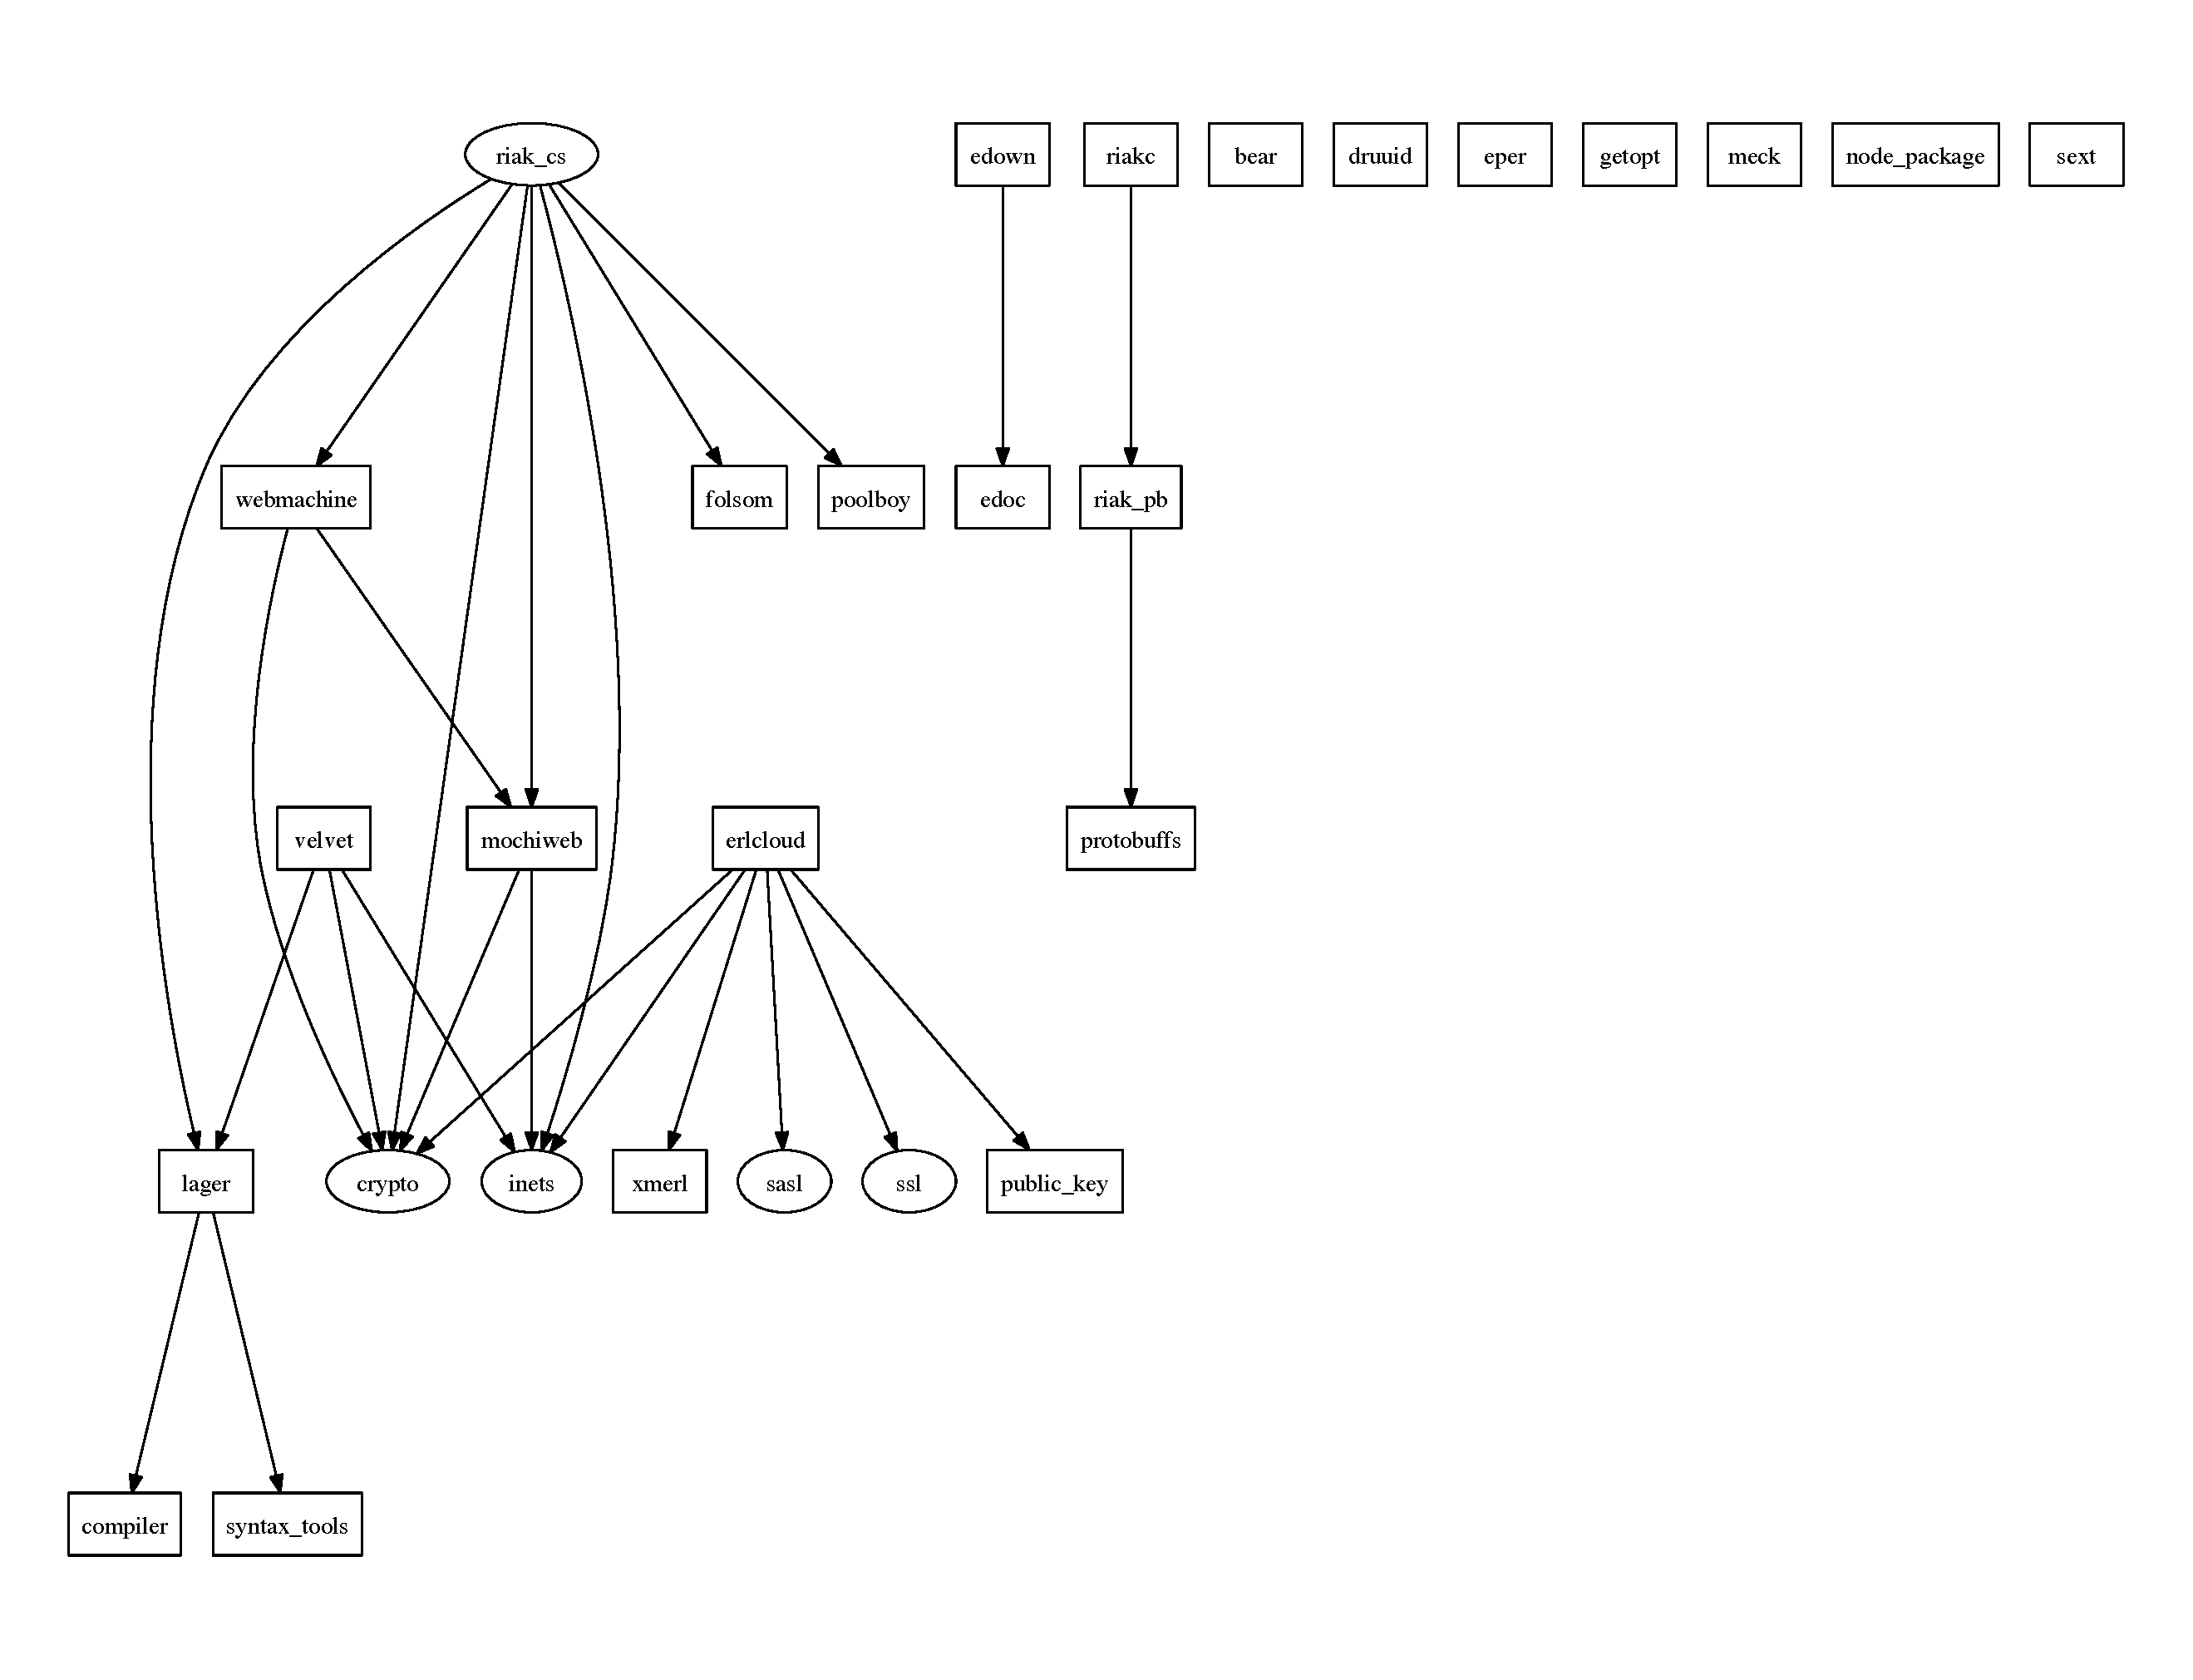
\includegraphics{app-deps-riak-cs.pdf}%
  \caption{Dependency graph of riak\_cs, Basho's open source cloud library.
  The graph has been generated with recon's app\_deps script, and ignores dependencies on common applications like kernel and stdlib. Ovals are applications, rectangles are library applications.}%
   \label{fig:app-deps}
\end{figure}

Using such a hierarchy and looking at each application's short description might be helpful to draw a rough, general map of where everything is located. To generate a similar diagram, find recon's script directory and call \command{escript ./deps/recon/script/app\_deps.erl}\footnote{This script depends on graphviz}. Similar hierarchies can be found using the \module{observer}\footnote{\href{http://www.erlang.org/doc/apps/observer/observer\_ug.html}{http://www.erlang.org/doc/apps/observer/observer\_ug.html}} application, but for individual supervision trees. Put together, you may get an easy way to find out what does what in the code base.

\FloatBarrier

\section{OTP Releases}
\label{sec:dive-otp-releases}

OTP releases are not a lot harder to understand than most OTP applications in the wild. A release is a set of OTP applications packaged in a production-ready manner so it boots and shuts down without needing to manually call \function{application:start/2} for any app. Of course there's a bit more to releases than that, but generally, the same discovery process used for individual OTP applications will be applicable here.

You'll usually have a file similar to the configuration files used by \module{systools} or \module{reltool}, which will state all applications part of the release and a few\footnote{a lot} options regarding their packaging. To understand them, I recommend \href{http://learnyousomeerlang.com/release-is-the-word}{reading existing documentation on them}. If you're lucky, the project may be using \app{relx}\footnote{\href{https://github.com/erlware/relx/wiki}{https://github.com/erlware/relx/wiki}}, an easier tool that was officially released in early 2014.


\section{Exercises}

\subsection{Review Questions}

\begin{enumerate}
	\item How do you know if a code base is an application? A release?
	\item What differentiates an application from a library application?
	\item What can be said of processes under a \term{one\_for\_all} scheme for supervision?
	\item Why would someone use a \module{gen\_fsm} behaviour over a \module{gen\_server}?
\end{enumerate}

\subsection{Hands-On}

Download the code at \href{https://github.com/ferd/recon\_demo}{https://github.com/ferd/recon\_demo}. This will be used as a test test bed for exercises throughout the book. Given you are not familiar with the code base yet, let's see if you can use the tips and tricks mentioned in this chapter to get an understanding of it.

\begin{enumerate}
	\item Is this application meant to be used as a library? A standalone system?
	\item What does it do?
	\item Does it have any dependencies? What are they?
	\item The app's \filename{README} mentions being non-deterministic. Can you prove if this is true? How?
	\item Can you express the dependency chain of applications in there? Generate a diagram of them?
	\item Can you add more processes to the main application than those described in the \filename{README}? 
\end{enumerate}
%%%
%%%
%%%

%%% Cognitive
%%
%% Knowledge: recall facts, terms, basic concepts
%% 
%% - How do you know if a code base is an application? A release?
%% - Where can you find what an application does?
%% - What differentiates an application from a library application?
%%
%% Comprehension: organizing, comparing, translating, interpreting, giving descriptions, and stating the main ideas
%%
%% - What can be said of processes under a one_for_all scheme for supervision?
%% - Why would someone use a gen_fsm process over a gen_server?
%%
%% Application: Solve problems in new situations by applying acquired knowledge, facts, techniques and rules in a different way
%%
%% Using the code at: https://github.com/ferd/recon_demo
%% - Is this application meant to be used as a library? A standalone system?
%% - What does it do?
%% - Does it have any dependencies? What are they?
%%
%% Analysis: break down info, make inferences, find evidence
%% - The app's readme mentions being non-deterministic. Can you prove if this is true? How?
%% - Can you express the dependency chain of applications in there? Generate a diagram of them?
%%
%% Synthesis: Compile information together in a different way by combining elements in a new pattern or proposing alternative solutions
%%
%% - Can you add more processes to the application? DO IT!
%%
%% Evaluation: Present and defend opinions by making judgments about information
%%
%% - Do you think the method you've chosen to add applications would work well operationally to be done live? If not, is this due to your choice or the application structure? 
%%

%%%
%%%
%%%

\chapter{Building Open Source Erlang Software}
\label{chap:building-open-source-erlang-software}

Most Erlang books tend to explain how to build Erlang and OTP applications, but few of them go very much in depth about how to integrate with the Erlang community doing Open Source work. Some of them even avoid the topic on purpose. This chapter dedicates itself to doing a quick tour of the state of affairs in Erlang.

OTP applications are the vast majority of the open source code people will encounter. In fact, many people who would need to build an OTP release would do so as one umbrella OTP application. 

If what you're writing is a stand-alone piece of code that could be used by someone building a product, it's likely an OTP application. If what you're building is a product that stands on its own and should be deployed by users as-is (or with a little configuration), what you should be building is an OTP release.\footnote{The details of how to build and OTP application or release is left up to the Erlang introduction book you have at hand.}

The main build tools supported are \app{rebar} and \app{erlang.mk}. The former is a portable Erlang script that will be used to wrap around a lot of standard functionality and add its own, while the latter is a very fancy makefile that does a bit less, but tends to be faster when it comes to compiling. In this chapter, I'll mostly focus on using \app{rebar} to build things, given it's the ad-hoc standard, is well-established, and \app{erlang.mk} applications tend to also be supported by \app{rebar} as dependencies.

\section{Project Structure}
\label{sec:project-structure}

The structures of OTP applications and of OTP releases are different. An OTP application can be expected to have one top-level supervisor (if any) and possibly a bunch of dependencies that sit below it. An OTP release will usually be composed of multiple OTP applications, which may or may not depend on each other. This will lead to two major ways to lay out applications.

\subsection{OTP Applications}
\label{subsec:building-otp-applications}

For OTP applications, the proper structure is pretty much the same as what was explained in \ref{sec:dive-otp-applications}:

\begin{VerbatimText}
doc/
deps/
ebin/
src/
test/
LICENSE.txt
README.md
rebar.config
\end{VerbatimText}

What's new in this one is the \filename{deps/} directory, which is fairly useful to have, but that will be generated automatically by \app{rebar}\footnote{A lot of people package \app{rebar} directly in their application. This was initially done to help people who never used rebar before use libraries and projects in a boostrapped manner. Feel free to install rebar globally on your system, or keep a local copy if you require a specific version to build your system.} if necessary. That's because there is no canonical package management in Erlang. People instead adopted what \app{rebar} provided, which was that you fetch dependencies locally, on a per-project basis. This is fine and removes a truckload of conflicts, but means that each project you have may have to download its own set of dependencies.

This is accomplished with \app{rebar} by adding a few config lines to \filename{rebar.config}:

\begin{VerbatimText}
{deps,
 [{application_name, "1.0.*",
   {git, "git://github.com/user/myapp.git", {branch,"master"}}},
  {application_name, "2.0.1",
   {git, "git://github.com/user/hisapp.git", {tag,"2.0.1"}}},
  {application_name, "", 
   {git, "https://bitbucket.org/user/herapp.git",  "7cd0aef4cd65"}},
  {application_name, "my regex",
   {hg, "https://bitbucket.org/user/theirapp.hg" {branch, "stable"}}}]}.
\end{VerbatimText}

Applications are fetched directly from a \app{git} (or \app{hg}, or \app{svn}) source, recursively. They can then be compiled, and specific compile options can be added with the \expression{\{erl\_opts, List\}.} option in the config file\footnote{More details by calling \command{rebar help compile}}. 

Within these directories, you can do your regular development of an OTP application. To compile them, call \command{rebar get-deps compile}, which will download all dependencies, and then build them and your app at once.

When making your application public to the world, distribute it \emph{without} the dependencies. It's quite possible that other developers' applications depend on the same applications yours do, and it's no use shipping them all multiple times. The build system in place (in this case, \app{rebar}) should be able to figure out duplicated entries and fetch everything necessary only once.

%% erlang.mk downloads relx for releases, and runs it iff there's a relx file there

\subsection{OTP Releases}
\label{subsec:building-otp-releases}

For releases, the structure should be a bit different\footnote{I say \emph{should} because many Erlang developers put their final system under a single top-level application (in \filename{src}) and a bunch of follower ones as dependencies (in \filename{deps}), which is less than ideal for distribution purposes and conflicts with assumptions on directory structures made by OTP. People who do that tend to build from source on the production servers and run custom commands to boot their applications.}. Releases are collections of applications, and their structures should reflect that.

Instead of having a top-level app, applications should be nested one level deeper and divided into two categories: apps and deps. The apps directory contains your applications' source code (say, internal business code), and the deps directory contains independently managed dependency applications.

\begin{VerbatimRaw}
apps/
doc/
deps/
LICENSE.txt
README.md
rebar.config
\end{VerbatimRaw}

This structure lends itself to generating releases. Tools such as Systool and Reltool have been covered before\footnote{\href{http://learnyousomeerlang.com/release-is-the-word}{http://learnyousomeerlang.com/release-is-the-word}}, and can allow the user plenty of power. An easier tool that recently appeared is \app{relx}\footnote{\href{https://github.com/erlware/relx/wiki}{https://github.com/erlware/relx/wiki}}.

A  \app{relx} configuration file for the directory structure above would look like:

\begin{VerbatimText}
{paths, ["apps", "deps"]}.
{include_erts, false}. % will use currently installed Erlang
{default_release, demo, "1.0.0"}.

{release, {demo, "1.0.0"},
    [members,
     feedstore,
     ...
     recon]}.
\end{VerbatimText}

Calling \command{./relx} (if the executable is in the current directory) will build a release, to be found in the \filename{\_rel/} directory. If you really like using \app{rebar}, you can build a release as part of the project's compilation by using a rebar hook in \filename{rebar.config}:

\begin{VerbatimText}
{post_hooks,[{compile, "./relx"}]}.
\end{VerbatimText}

And every time \command{rebar compile} will be called, the release will be generated.

\section{Supervisors and start\_link Semantics}
\label{sec:supervisors-and-start-link-semantics}

In complex production systems, most faults and errors are transient, and retrying an operation is a good way to do things — Jim Gray's paper\footnote{\href{http://mononcqc.tumblr.com/post/35165909365/why-do-computers-stop}{http://mononcqc.tumblr.com/post/35165909365/why-do-computers-stop}} quotes \emph{Mean Times Between Failures} (MTBF) of systems handling transient bugs being better by a factor of 4 when doing this. Still, supervisors aren't just about restarting.

One very important part of Erlang supervisors and their supervision trees is that \emph{their start phases are synchronous}. Each OTP process has the potential to prevent its siblings and cousins from booting. If the process dies, it's retried again, and again, until it works, or fails too often.

That's where people make a very common mistake. There isn't a backoff or cooldown period before a supervisor restarts a crashed child. When a network-based application tries to set up a connection during its initialization phase and the remote service is down, the application fails to boot after too many fruitless restarts. Then the system may shut down.

Many Erlang developers end up arguing in favor of a supervisor that has a cooldown period. I strongly oppose the sentiment for one simple reason: \emph{it's all about the guarantees}.

\subsection{It's About the Guarantees}
\label{subsec:start-link-guarantees}

Restarting a process is about bringing it back to a stable, known state. From there, things can be retried. When the initialization isn't stable, supervision is worth very little. An initialized process should be stable no matter what happens. That way, when its siblings and cousins get started later on, they can be booted fully knowing that the rest of the system that came up before them is healthy.

If you don't provide that stable state, or if you were to start the entire system asynchronously, you would get very little benefit from this structure that a \expression{try ... catch} in a loop wouldn't provide.

Supervised processes \emph{provide guarantees} in their initialization phase, \emph{not a best effort}. This means that when you're writing a client for a database or service, you shouldn't need a connection to be established as part of the initialization phase unless you're ready to say it will always be available no matter what happens.

You could force a connection during initialization if you know the database is on the same host and should be booted before your Erlang system, for example. Then a restart should work. In case of something incomprehensible and unexpected that breaks these guarantees, the node will end up crashing, which is desirable: a pre-condition to starting your system hasn't been met. It's a system-wide assertion that failed.

If, on the other hand, your database is on a remote host, you should expect the connection to fail. It's just a reality of distributed systems that things go down.\footnote{Or latency shoots up enough that it is impossible to tell the difference from failure.} In this case, the only guarantee you can make in the client process is that your client will be able to handle requests, but not that it will communicate to the database. It could return \expression{\{error, not\_connected\}} on all calls during a net split, for example.

The reconnection to the database can then be done using whatever cooldown or backoff strategy you believe is optimal, without impacting the stability of the system. It can be attempted in the initialization phase as an optimization, but the process should be able to reconnect later on if anything ever disconnects.

If you expect failure to happen on an external service, do not make its presence a guarantee of your system. We're dealing with the real world here, and failure of external dependencies is always an option. To put it another way, we're going to lean on liveness (something good should eventually happen) as a guarantee, and reduce the safety (something bad will never happen) that we promise when it comes to the availability of services in a distributed system.

\subsection{Side Effects}
\label{subsec:start-link-side-effects}

Of course, the libraries and processes that call such a client will then error out if they don't expect to work without a database. That's an entirely different issue in a different problem space, but one that is possible to work around. For example, consider a client for a service that stores operational metrics — the code that calls that client could very well ignore the errors without adverse effects to the system as a whole. 

The difference in both initialization and supervision approaches is that the client's callers make the decision about how much failure they can tolerate, not the client itself. That's a very important distinction when it comes to designing fault-tolerant systems. Yes, supervisors are about restarts, but they should be about restarts to a stable known state.

\subsection{Example: Initializing without guaranteeing connections}
\label{subsec:start-link-initializing-without-guaranteeing-connections}

The following code attempts to guarantee a connection as part of the process' state:

\begin{VerbatimText}
init(Args) ->
    Opts = parse_args(Args),
    {ok, Port} = connect(Opts),
    {ok, #state{sock=Port, opts=Opts}}.

[...]

handle_info(reconnect, S = #state{sock=undefined, opts=Opts}) ->
    case connect(Opts) of
        {ok, New} -> {noreply, S#state{sock=New}};
         _ -> self() ! reconnect, {noreply, S}
    end;
\end{VerbatimText}

Instead, consider rewriting it as:

\begin{VerbatimText}
init(Args) ->
    Opts = parse_args(Args),
    %% you could try connecting here anyway, for a best
    %% effort thing, but be ready to not have a connection.
    self() ! reconnect,
    {ok, #state{sock=undefined, opts=Opts}}.

[...]

handle_info(reconnect, S = #state{sock=undefined, opts=Opts}) ->
    case connect(Opts) of
        {ok, New} -> {noreply, S#state{sock=New}};
        _ -> self() ! reconnect, {noreply, S}
    end;
\end{VerbatimText}

You now allow initializations with fewer guarantees: they went from \emph{the connection is available} to \emph{the connection manager is available}.

\subsection{In a nutshell}
\label{subsec:start-link-in-a-nutshell}

Production systems I have worked with have been a mix of both approaches.

Things like configuration files, accessibility to the file system (say for logging purposes), local resources that can be depended on (opening UDP ports for logs), restoring a stable state from disk or network, and so on, are things I'll put into requirements of a supervisor and may decide to synchronously load no matter how long it takes (some applications may just end up having over 10 minute boot times in rare cases, but that's okay because we're possibly syncing gigabytes that we \emph{need} to work with as a base state if we don't want to serve incorrect information.)

On the other hand, code that depends on non-local databases and external services will adopt partial startups with quicker supervision tree booting because if the failure is expected to happen often during regular operations,
then there's no difference between now and later. You have to handle it the same, and for these parts of the system, far less strict guarantees are often the better solution.

\subsection{Application Strategies}
\label{subsec:start-link-application-strategies}

No matter what, a sequence of failures is not a death sentence for the node. Once a system has been divided into various OTP applications, it becomes possible to choose which applications are vital or not to the node. Each OTP application can be started in 3 ways: temporary, transient, permanent, either by doing it manually in \expression{application:start(Name, Type)}, or in the config file for your release:

\begin{itemize*}
	\item \term{permanent}: if the app terminates, the entire system is taken down, excluding manual termination of the app with \function{application:stop/1}.
	\item \term{transient}: if the app terminates for reason 'normal', that's ok. Any other reason for termination shuts down the entire system.
	\item \term{temporary}: the application is allowed to stop for any reason. It will be reported, but nothing bad will happen.
\end{itemize*}

It is also possible to start an application as an \emph{included application}, which starts it under your own OTP supervisor with its own strategy to restart it.

\section{Exercises}

\subsection{Review Questions}

\begin{enumerate}
	\item  Are Erlang supervision trees started depth-first? breadth-first? Synchronously or asynchronously?
	\item What are the three application strategies? What do they do?
	\item What are the main differences between the directory structure of an app and a release?
	\item When should you use a release?
	\item Give two examples of the type of state that can go in a process' init function, and two examples of the type of state that shouldn't go in a process' init function
\end{enumerate}

\subsection{Hands-On}

Using the code at \href{https://github.com/ferd/recon\_demo}{https://github.com/ferd/recon\_demo}:

\begin{enumerate}
	\item Extract the main application hosted in the release to make it independent, and includable in other projects.
	\item Host the application somewhere (Github, Bitbucket, local server), and build a release with that application as a dependency.
	\item The main application's workers (\module{council\_member}) starts a server and connects to it in its \function{init/1} function. Can you make this connection happen outside of the init function's? Is there a benefit to doing so in this specific case?
\end{enumerate}

%%
%% Knowledge: recall facts, terms, basic concepts
%% 
%% - Does Erlang have package management? Where do dependencies live in a system?
%% - What are the commands to build an Erlang project using rebar?
%% - What tools are available to build releases?
%% - Are Erlang supervision trees started depth-first? breadth-first? Synchronously or asynchronously?
%% - What are the three application strategies?
%%
%% Comprehension: organizing, comparing, translating, interpreting, giving descriptions, and stating the main ideas
%%
%% - What are the main differences between the directory structure of an app? of a release?
%% - When should you use a release?
%%
%% Application: Solve problems in new situations by applying acquired knowledge, facts, techniques and rules in a different way
%%
%% Using the code at: https://github.com/ferd/recon_demo
%% - Extract the main application hosted in the release to make it independent, and includable in other projects
%% - Build a release with the app that was turned as a dependency
%%
%% Analysis: break down info, make inferences, find evidence
%% - Give two examples of the type of state that can go in a process' init function
%% - Give two examples of the type of state that should not go in a process' init function
%%
%% Synthesis: Compile information together in a different way by combining elements in a new pattern or proposing alternative solutions
%%
%% - Give example of applications you would design as temporary, transient, and permanent
%%
%% Evaluation: Present and defend opinions by making judgments about information
%%
%% - Do you think OTP supervisors should offer a back-off strategy on restart?
%% - What are the build tools you would choose for your app?
%%

%%%
%%%
%%%


\chapter{Planning for Overload}
\label{chap:overload}

By far, the most common cause of failure I've encountered in real-world scenarios is due to the node running out of memory. Furthermore, it is usually related to message queues going out of bounds.\footnote{Figuring out that a message queue is the problem is explained in Chapter \ref{chap:crash-dumps}, specifically in Section \ref{sec:crash-full-mailboxes}} There are plenty of ways to deal with this, but knowing which one to use will require a decent understanding of the system you're working on.

To oversimplify things, most of the projects I end up working on can be visualized as a very large bathroom sink. User and data input are flowing from the faucet. The Erlang system itself is the sink and the pipes, and wherever the output goes (whether it's a database, an external API or service, and so on) is the sewer system.

\begin{figure}
  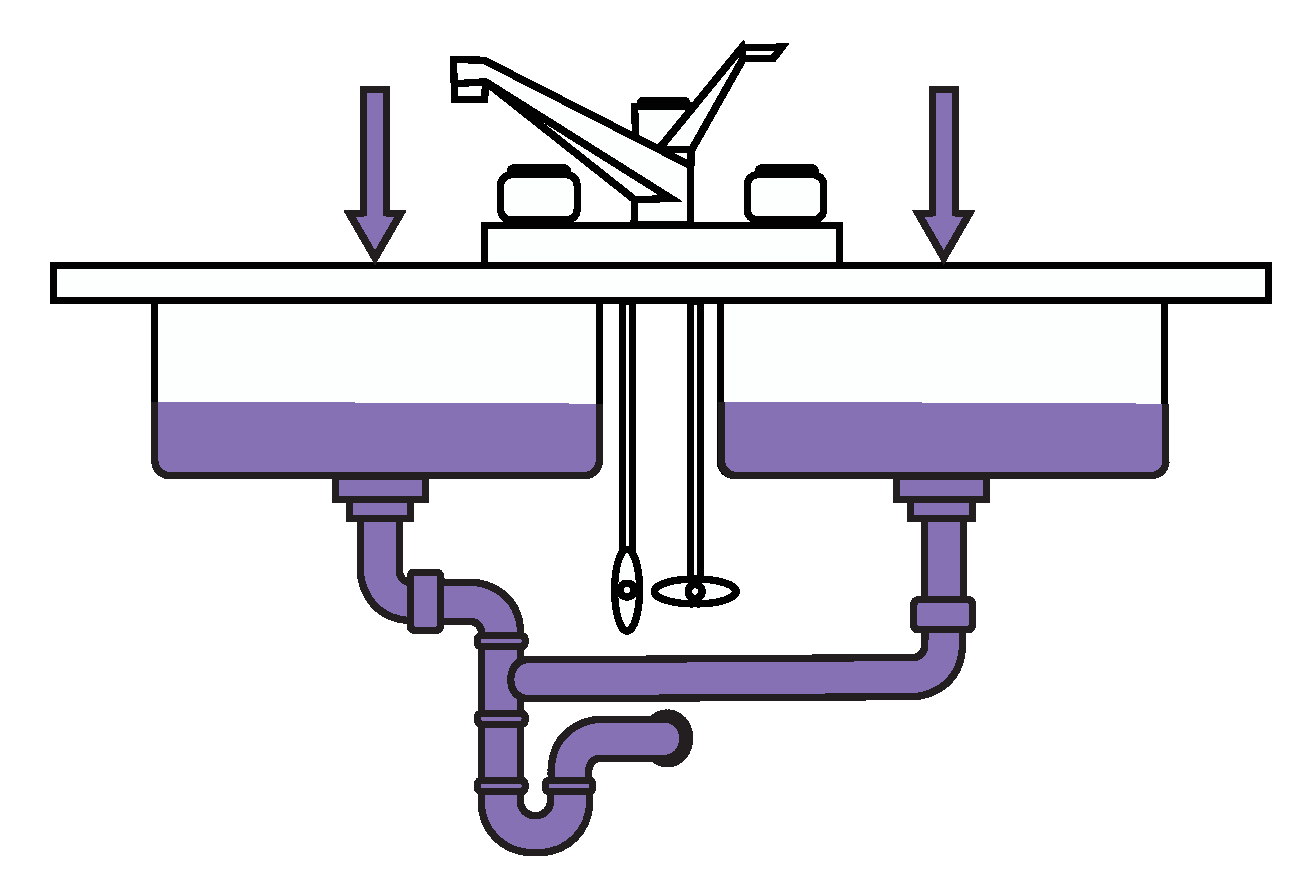
\includegraphics[max height=7cm]{sink.pdf}%
  \centering%
  \caption{Your system is like a sink, and the true bottleneck, at the last drain, needs to be identified before you spend all your time and money making the sink and pipes bigger.}%
   \label{fig:tracing-venn}
\end{figure}

When an Erlang node dies because of a queue overflowing, figuring out who to blame is crucial. Did someone put too much water in the sink? Are the sewer systems backing up? Did you just design too small a pipe?

Determining what queue blew up is not necessarily hard. This is information that can be found in a crash dump. Finding out why it blew up is trickier. Based on the role of the process or run-time inspection, it's possible to figure out whether causes include fast flooding, blocked processes that won't process messages fast enough, and so on.

The most difficult part is to decide how to fix it. When the sink gets clogged up by too much waste, we will usually start by trying to make the sink itself larger (the part of our program that crashed, at the edge). Then we figure out the sink's drain is too small, and optimize that. Then we find out the pipes themselves are too narrow, and optimize that. The overload gets pushed further down the system, until the sewers can't take it anymore. At that point, we may try to add sinks or various locations to help with the global input level.

Then there's a point where things can't be improved anymore at the bathroom's level. There are too many logs sent around, there's a bottleneck on databases that \emph{need} the consistency, or there's simply not enough knowledge or manpower in your organization to improve things there.

\FloatBarrier

We identified what the \emph{true bottleneck} of the system was, and all the prior optimization was nice, but it was more or less in vain.

We need to be more clever, and so things are moved back up a level. We try to massage the information going in the system to make it either lighter (whether it is through compression, better algorithms and data representation, caching, and so on). Even then, there are times where overload will be too much, and we have to make the hard decisions between restricting the input to the system, discarding it, or accepting that the system will reduce its quality of service up to the point it will crash.

In this chapter, we will explore common causes of queues blowing up, along with two broad strategies to deal with the issue in general: back-pressure and load-shedding.

\section{Common Overload Sources}

There are a few common causes of queues blowing up and overload in Erlang systems that most people will encounter sooner or later, no matter how they approach their system. They're usually symptomatic of having your system grow up and require some help scaling up, or of an unexpected type of failure that ends up cascading much harder than it should have.

\subsection{error\_logger Explodes}

Ironically, the process in charge of error logging is one of the most fragile ones. In a default Erlang install, the \module{error\_logger}\footnote{defined at \href{http://www.erlang.org/doc/man/error\_logger.html}{http://www.erlang.org/doc/man/error\_logger.html}} process will take its sweet time to log things to disk or over the network, and will do so much more slowly than errors can be generated.

This is especially true of user-generated log messages (not for errors), and for crashes in large processes. For the former, this is because \module{error\_logger} doesn't really expect arbitrary levels of messages coming in continually. It's for exceptional cases only and doesn't expect lots of traffic. For the latter, it's because the entire state of processes (including their mailboxes) gets copied over to be logged. It only takes a few messages to cause memory to bubble up a lot, and if that's not enough to cause the node to run Out Of Memory (OOM), it may slow the logger enough that additional messages will.

The best solution for this at the time of writing is to use \href{https://github.com/basho/lager}{\module{lager}} as a substitute logging library.

While Lager will not solve all your problems, it will truncate voluminous log messages, optionally drop OTP-generated error messages when they go over a certain threshold, and will automatically switch between asynchronous and synchronous modes for user-submitted messages in order to self-regulate.

It won't be able to deal with very specific cases, such as when user-submitted messages are in very large volume and all coming from one-off processes. This is, however, a much rarer occurrence than everything else, and one where the programmer tends to have more control.


\subsection{Locks and Blocking Operations}

Locking and blocking operations will often be problematic when they're taking unexpectedly long to execute in a process that's constantly receiving new tasks.

One of the most common examples I've seen is a process blocking while accepting a connection or waiting for messages with TCP sockets. During blocking operations of this kind, messages are free to pile up in the message queue.

One particularly bad example was in a pool manager for HTTP connections that I had written in a fork of the \href{https://github.com/ferd/lhttpc}{\module{lhttpc}} library. It worked fine in most test cases we had, and we even had a connection timeout set to 10 milliseconds to be sure it never took too long\footnote{10 milliseconds is very short, but was fine for collocated servers used for real-time bidding.}. After a few weeks of perfect uptime, the HTTP client pool caused an outage when one the remote servers went down.

The reason behind this degradation was that when the remote server would go down, all of a sudden, all connecting operations would take at least 10 milliseconds, the time before which the connection attempt is given up on. With around 9,000 messages per second to the central process, each usually taking under 5 milliseconds, the impact became similar to roughly 18,000 messages a second and things got out of hand.

The solution we came up with was to leave the task of connecting to the caller process, and enforce the limits as if the manager had done it on its own. The blocking operations were now distributed to all users of the library, and even less work was required to be done by the manager, now free to accept more requests.

When there is \emph{any} point of your program that ends up being a central hub for receiving messages, lengthy tasks should be moved out of there if possible. Handling predictable overload\footnote{Something you know for a fact gets overloaded in production} situations by adding more processes — which either handle the blocking operations or instead act as a buffer while the "main" process blocks — is often a good idea.

There will be increased complexity in managing more processes for activities that aren't technically concurrent, so make sure you need them before programming defensively.

Another option is to transform the blocking task into an asynchronous one. If the type of work allows it, start the long-running job and keep a token that identifies it uniquely, along with the original requester you're doing work for. When the resource is available, have it send a message back to the server with the aforementioned token. The server will eventually get the message, match the token to the requester, and answer back, without being blocked by other requests in the mean time.\footnote{The \otpapp{redo} application is an example of a library doing this, in its \href{https://github.com/heroku/redo/blob/master/src/redo\_block.erl}{redo\_block} module. The [under-documented] module turns a pipelined connection into a blocking one, but does so while maintaining pipeline aspects to the caller — this allows the caller to know that only one call failed when a timeout occurs, not all of the in-transit ones, without having the server stop accepting requests.}

This option tends to be more obscure than using many processes and can quickly devolve into callback hell, but may use fewer resources.

\subsection{Unexpected Messages}

Messages you didn't know about tend to be rather rare when using OTP applications. Because OTP behaviours pretty much expect you to handle anything with some clause in \function{handle\_info/2}, unexpected messages will not accumulate much.

However, all kinds of OTP-compliant systems end up having processes that may not implement a behaviour, or processes that go in a non-behaviour stretch where it overtakes message handling. If you're lucky enough, monitoring tools\footnote{See Section \ref{sec:global-view}} will show a constant memory increase, and inspecting for large queue sizes\footnote{See Subsection \ref{subsec:digging-procs}} will let you find which process is at fault. You can then fix the problem by handling the messages as required.

\section{Generally Restricting Input}

Restricting input is the simplest way to manage message queue growth in Erlang systems. It's the simplest approach because it basically means you're slowing the user down (applying \emph{back-pressure}), which instantly fixes the problem without any further optimization required. On the other hand, it can lead to a really crappy experience for the user.

The most common way to restrict data input is to make calls to a process whose queue would grow in uncontrollable ways synchronously. By requiring a response before moving on to the next request, you will generally ensure that the direct source of the problem will be slowed down.

The difficult part for this approach is that the bottleneck causing the queue to grow is usually not at the edge of the system, but deep inside it, which you find after optimizing nearly everything that came before. Such bottlenecks will often be database operations, disk operations, or some service over the network. 

This means that when you introduce synchronous behaviour deep in the system, you'll possibly need to handle back-pressure, level by level, until you end up at the system's edges and can tell the user, "please slow down."
Developers that see this pattern will often try to put API limits per user\footnote{There's a tradeoff between slowing down all requests equally or using rate-limiting, both of which are valid. Rate-limiting per user would mean you'd still need to increase capacity or lower the limits of all users when more new users hammer your system, whereas a synchronous system that indiscriminately blocks should adapt to any load with more ease, but possibly unfairly.} on the system entry points. This is a valid approach, especially since it can guarantee a basic quality of service (QoS) to the system and allows one to allocate resources as fairly (or unfairly) as desired.
  
\subsection{How Long Should a Time Out Be}

What's particularly tricky about applying back-pressure to handle overload via synchronous calls is having to determine what the typical operation should be taking in terms of time, or rather, at what point the system should time out.

The best way to express the problem is that the first timer to be started will be at the edge of the system, but the critical operations will be happening deep within it. This means that the edge of the system's timers will need to have longer timers, unless you plan on having operations time out even though they succeeded.

An easy way out of this is to go for infinite timeouts. Pat Helland\footnote{\href{http://queue.acm.org/detail.cfm?id=2187821}{Idempotence is Not a Medical Condition}, April 14, 2012} has an interesting answer to this:

\begin{quote}
Some application developers may push for no timeout and argue it is OK to wait indefinitely. I typically propose they set the timeout to 30 years. That, in turn, generates a response that I need to be reasonable and not silly. \emph{Why is 30 years silly but infinity is reasonable?} I have yet to see a messaging application that really wants to wait for an unbounded period of time…
\end{quote}

This is, ultimately, a case-by-case issue. In many cases, it may be interesting to use a different mechanism for that flow control.\footnote{In Erlang, using the value \term{infinity} will avoid creating a timer, avoiding some resources. If you do use this, remember to at least have a well-defined timeout somewhere in the sequence of calls.}

\subsection{Asking For Permission}

A somewhat simpler approach is to identify the resources we want to block on, those that cannot be made faster and are critical to your business and users, and lock them behind a module or procedure where a caller must ask for the right to make a request and use them. There's plenty of variables that can be used: memory, CPU, overall load, a bounded number of calls, concurrency, response times, a combination of them, and so on.

The \emph{SafetyValve}\footnote{\href{https://github.com/jlouis/safetyvalve}{https://github.com/jlouis/safetyvalve}} application is a system-wide framework that can be used when you know the synchronous approach is the one you'll need.

Otherwise, ad-hoc solutions can be written using processes, ETS, or any other tool available. The important part is that the edge of the system (or subsystem) may block and ask for the right to process data, but the critical bottleneck in code is the one to determine whether that right can be granted or not.

The advantage of proceeding that way is that you may just avoid all the tricky stuff about timers and making every single layer of abstraction synchronous. You'll instead put guards at the bottleneck and at a given edge or control point, and everything in between can be expressed in the most readable way possible.

\subsection{What Users See}

The tricky part about back-pressure is reporting it. When back-pressure is done implicitly through synchronous calls, the only way to know it is at work due to overload is that the system becomes slower and less usable. Sadly, this is also going to be a potential symptom of bad hardware, bad network, unrelated overload, and possibly a slow client.

Trying to figure out that a system is applying back-pressure by measuring its responsiveness is equivalent to trying to diagnose which illness someone has by observing that person has a fever. It tells you something is wrong, but not what.

Asking for permission, as a mechanism, will generally allow you to define your interface in such a way that you can explicitly report what is going on: the system as a whole is overloaded, or you're hitting a limit into the rate at which you can perform an operation and adjust accordingly.

There is a choice to be made when designing the system. Are your users going to have per-account limits, or are the limits going to be global to the system?

System-global or node-global limits are usually easy to implement, but will have the downside that they may be unfair. A user doing 90\% of all your requests may end up making the platform unusable for the vast majority of the other users.

Per-account limits, on the other hand, tend to be very fair, and allow fancy schemes such as having premium users who can go above the usual limits. This is extremely nice, but has the downside that the more users use your system, the higher the effective global system limit tends to move. Starting with 100 users that can do 100 requests a minute gives you a global 10000 requests per minute. Add 20 new users with that same rate allowed, and suddenly you may crash a lot more often.

The safe margin of error you established when designing the system slowly erodes as more people use it. It's important to consider the tradeoffs your business can tolerate from that point of view, because users will tend not to appreciate seeing their allowed usage go down all the time, possibly even more so than seeing the system go down entirely from time to time.


\section{Generally Discarding Data}

When nothing can slow down outside of your Erlang system and things can't be scaled up, you must either drop data or crash (which drops data that was in flight, for most cases, but with more violence).

It's a sad reality that nobody really wants to deal with. Programmers, software engineers, and computer scientists are trained to purge the useless data, and keep everything that's useful. Success goes through optimization, not giving up.

However, there's a point that can be reached where the data that comes in does so at a rate faster than it comes out, even if the Erlang system on its own is able to do everything fast enough. In some cases, It's the component \emph{after} it that blocks.

If you don't have the option of limiting how much data you receive, you then have to drop messages to avoid crashing.

\subsection{Random Drop}

Randomly dropping messages is the easiest way to do such a thing, and might also be the most robust implementation, due to its simplicity.

The trick is to define some threshold value between 0.0 and 1.0 and to fetch a random number in that range:

\includecode[erlang]{drop.erl}

If you aim to keep 95\% of the messages you send, the authorization could be written by a call to \expression{case drop:random(0.95) of true -> send(); false -> drop() end}, or a shorter \expression{drop:random(0.95) andalso send()} if you don't need to do anything specific when dropping a message. 

The \function{maybe\_seed()} function will check that a valid seed is present in the process dictionary and use it rather than a crappy one, but only if it has not been defined before, in order to avoid calling \function{now()} (a monotonic function that requires a global lock) too often.

There is one 'gotcha' to this method, though: the random drop must ideally be done at the producer level rather than at the queue (the receiver) level. The best way to avoid overloading a queue is to not send data its way in the first place. Because there are no bounded mailboxes in Erlang, dropping in the receiving process only guarantees that this process will be spinning crazily, trying to get rid of messages, and fighting the schedulers to do actual work.

On the other hand, dropping at the producer level ensures that the dropping work is distributed equally across all processes.

This can give place to interesting optimizations where the working process or a given monitor process\footnote{any process tasked with checking the load of specific processes using heuristics such as \expression{process\_info(Pid, message\_queue\_len)} could be a monitor} uses values in an ETS table or \function{application:set\_env/3} to dynamically increase and decrease the threshold to be used with the random number. This allows control over how many messages are dropped based on overload, and the configuration data can be fetched by any process rather efficiently by using \function{application:get\_env/2}.

Similar techniques could also be used to implement different drop ratios for different message priorities, rather than trying to sort it all out at the consumer level.

\subsection{Queue Buffers}

Queue buffers will be a good alternative when you want more control over the messages you get rid of than with random drops, particularly when you expect overload to be coming in bursts rather than a constant stream in need of thinning.

Even though the regular mailbox for a process has the form of a queue, you'll generally want to pull \emph{all} the messages out of it as soon as possible. A queue buffer will need two processes to be safe:

\begin{itemize*}
	\item The regular process you'd work with (likely a \module{gen\_server});
	\item A new process that will do nothing but buffer the messages. Messages from the outside should go to this process.
\end{itemize*}

To make things work, the buffer process only has to remove all the messages it can from its mail box and put them in a queue data structure\footnote{the \module{queue} module in Erlang provides a purely functional queue data structure that can work fine for such a buffer.}. Whenever the server is ready to do more work, it can ask the buffer to send it a given number of messages that it can work on. The buffer sends them, and goes back to accumulating data.


Whenever the queue grows beyond a certain size\footnote{To calculate the length of a queue, it is preferable to use a counter that gets incremented and decremented on each message sent or received, rather than iterating over the queue every time. It takes slightly more memory, but will tend to distribute the load of counting more evenly, helping predictability and avoiding more sudden build-ups in the buffer's mailbox} and you receive a new message, you can then pop the oldest one and push the new one in there, dropping the oldest elements as you go.\footnote{You can alternatively make a queue that pops the newest message and queues up the oldest ones if you feel previous data is more important to keep.}

This should keep the entire number of messages received to a rather stable size and provide a good amount of resistance to overload, somewhat similar to the functional version of a ring buffer.

The \emph{PO Box}\footnote{Available at: \href{https://github.com/ferd/pobox}{https://github.com/ferd/pobox}, the library has been used in production for a long time in large scale products at Heroku and is considered mature} library implements such a queue buffer.

\subsection{Stack Buffers}

Stack buffers are ideal when you want the amount of control offered by queue buffers, but you have an important requirement for low latency.

To use a stack as a buffer, you'll need two processes, just like you would with queue buffers, but a list\footnote{Erlang lists \emph{are} stacks. For all we care, they provide push and pop operations that take O(1) complexity and are very fast} will be used instead of a queue data structure.

The reason the stack buffer is particularly good for low latency is related to issues similar to bufferbloat\footnote{\href{http://queue.acm.org/detail.cfm?id=2071893}{http://queue.acm.org/detail.cfm?id=2071893 }}. If you get behind on a few messages being buffered in a queue, all the messages in the queue get to be slowed down and acquire milliseconds of wait time. Eventually, they all get to be too old and the entire buffer needs to be discarded.

%% Image of queue taking long from RTB article. Maybe side image or side explanation?

On the other hand, a stack will make it so only a restricted number of elements are kept waiting while the newer ones keep making it to the server to be processed in a timely manner.

%% image of queue taking a short time from RTB article.

Whenever you see the stack grow beyond a certain size or notice that an element in it is too old for your QoS requirements you can just drop the rest of the stack and keep going from there. \emph{PO Box} also offers such a buffer implementation.

If you need to react to old events \emph{before} they are too old, then things become more complex, as you can't know about it without looking deep in the stack each time, and dropping from the bottom of the stack in a constant manner gets to be inefficient. An interesting approach could be done with buckets, where multiple stacks are used, with each of them containing a given time slice. When requests get too old for the QoS constraints, drop an entire bucket, but not the entire buffer.

It may sound counter-intuitive to make some requests a lot worse to benefit the majority — you'll have great medians but poor 99 percentiles — but this happens in a state where you would drop messages anyway, and is preferable in cases where you do need low latency. 

A major downside of stack buffers is that messages are not necessarily going to be processed in the order they were submitted — they're nicer for independent tasks, but will ruin your day if you expect a sequence of events to be respected.

\subsection{Dealing With Constant Overload}

Being under constant overload may require a new solution. Whereas both queues and buffers will be great for cases where overload happens from time to time (even if it's a rather prolonged period of time), they both work more reliably when you expect the input rate to eventually drop, letting you catch up.

You'll mostly get problems when trying to send so many messages they can't make it all to one process without overloading it. Two approaches are generally good for this case:

\begin{itemize*}
	\item Have many processes that act as buffers and load-balance through them (scale horizontally)
	\item use ETS tables as locks and counters (reduce the input)
\end{itemize*}

ETS tables are generally able to handle a ton more requests per second than a process, but the operations they support are a lot more basic. A single read, or adding or removing from a counter atomically is as fancy as you should expect things to get for the general case.

ETS tables will be required for both approaches.

Generally speaking, the first approach could work well with the regular process registry: you take \var{N} processes to divide up the load, give them all a known name, and pick one of them to send the message to. Given you're pretty much going to assume you'll be overloaded, randomly picking a process with an even distribution tends to be reliable: no state communication is required, work will be shared in a roughly equal manner, and it's rather insensitive to failure.

In practice, though, we want to avoid atoms generated dynamically, so I tend to prefer to register things in an ETS table with \expression{read\_concurrency} set to \expression{true}. It's a bit more work, but it gives more flexibility when it comes to updating the number of workers later on.

An approach similar to this one is used in the \module{lhttpc}\footnote{the \href{https://github.com/ferd/lhttpc/blob/master/src/lhttpc\_lb.erl}{lhttpc\_lb} module in this library implements it.} library mentioned earlier, to split load balancers on a per-domain basis.

For the second approach, using counters and locks, the same basic structure still remains (pick one of many options, send it a message), but before actually sending a message, you must atomically update an ETS counter\footnote{By using \function{ets:update\_counter/3}.}. There is a known limit shared across all clients (either through their supervisor, or any other config or ETS value) and each request that can be made to a process needs to clear this limit first.

This approach has been used in \module{dispcount}\footnote{\href{https://github.com/ferd/dispcount}{https://github.com/ferd/dispcount}} to avoid message queues, and to guarantee low-latency responses to any message that won't be handled so that you do not need to wait to know your request was denied. It is then up to the user of the library whether to give up as soon as possible, or to keep retrying with different workers.

\subsection{How Do You Drop}

Most of the solutions outlined here work based on message quantity, but it's also possible to try and do it based on message size, or expected complexity, if you can predict it. When using a queue or stack buffer, instead of counting entries, all you may need to do is count their size or assign them a given load as a limit.

I've found that in practice, dropping without regard to the specifics of the message works rather well, but each application has its share of unique compromises that can be acceptable or not\footnote{Old papers such as \href{http://research.microsoft.com/en-us/um/people/blampson/33-hints/webpage.html}{Hints for Computer System Designs} by Butler W. Lampson recommend dropping messages: "Shed load to control demand, rather than allowing the system to become overloaded." The paper also mentions that  "A system cannot be expected to function well if the demand for any resource exceeds two-thirds of the capacity, unless the load can be characterized extremely well." adding that "The only systems in which cleverness has worked are those with very well-known loads."}.

There are also cases where the data is sent to you in a "fire and forget" manner — the entire system is part of an asynchronous pipeline — and it proves difficult to provide feedback to the end-user about why some requests were dropped or are missing. If you can reserve a special type of message that accumulates dropped responses and tells the user "\var{N} messages were dropped for reason \var{X}", that can, on its own, make the compromise far more acceptable to the user. This is the choice that was made with Heroku's \href{https://devcenter.heroku.com/articles/logplex}{logplex} log routing system, which can spit out \href{https://devcenter.heroku.com/articles/error-codes\#l10-drain-buffer-overflow}{L10 errors}, alerting the user that a part of the system can't deal with all the volume right now.

In the end, what is acceptable or not to deal with overload tends to depend on the humans that use the system. It is often easier to bend the requirements a bit than develop new technology, but sometimes it is just not avoidable.


\section{Exercises}

\subsection{Review Questions}

\begin{enumerate}
	\item Name the common sources of overload in Erlang systems
	\item What are the two main classes of strategies to handle overload?
	\item How can long-running operations be made safer?
	\item When going synchronous, how should timeouts be chosen?
	\item What is an alternative to having timeouts?
	\item When would you pick a queue buffer before a stack buffer?
\end{enumerate}

\subsection{Open-ended Questions}

\begin{enumerate}
	\item What is a \emph{true bottleneck}? How can you find it?
	\item In an application that calls a third party API, response times vary by a lot depending on how healthy the other servers are. How could one design the system to prevent occasionally slow requests from blocking other concurrent calls to the same service?
	\item What's likely to happen to new requests to an overloaded latency-sensitive service where data has backed up in a stack buffer? What about old requests?
	\item Explain how you could turn a load-shedding overload mechanism into one that can also provide back-pressure.
	\item Explain how you could turn a back-pressure mechanism into a load-shedding mechanism. 
	\item What are the risks, for a user, when dropping or blocking a request? How can we prevent duplicate messages or missed ones?
	\item What can you expect to happen to your API design if you forget to deal with overload, and suddenly need to add back-pressure or load-shedding to it?
\end{enumerate}


%%% Cognitive
%%
%% Knowledge: recall facts, terms, basic concepts
%% 
%% - Name the common sources of overload in Erlang systems
%% - What are the two main classes of strategies to handle overload?
%%
%% Comprehension: organizing, comparing, translating, interpreting, giving descriptions, and stating the main ideas
%%
%% - Why is it that error_logger may cause failures? How can they be fixed?
%% - When can long-running operations become problematic?
%% - How can long-running operations be made safer?
%% - When going synchronous, how should timeouts be chosen?
%% - What is an alternative to having timeouts?
%% - What are ways to communicate overload to users?
%% - What can you do when you can't slow down data input?
%% - Is there a different approach to be taken between temporary and permanent overload?
%%
%% Application: Solve problems in new situations by applying acquired knowledge, facts, techniques and rules in a different way
%%
%% - How can you find what is a 'true bottleneck' ?
%% - In an application that calls a third party API, response times vary by a lot depending on how healthy the other servers are. How could one design the system to prevent occasionally slow requests from blocking other ones?
%% - When would you pick a queue buffer before a stack buffer? 
%% - Which end should you drop items from in a queue buffer, and when?
%%
%% Analysis: break down info, make inferences, find evidence
%% - What's likely to happen to new requests to an overloaded latency-sensitive service where data has backed up in a stack buffer? What about old ones?
%% - What can you expect about response times if an app is permanently overloaded while using a queue buffer?
%% - 
%%
%% Synthesis: Compile information together in a different way by combining elements in a new pattern or proposing alternative solutions
%%
%% - Explain how you could turn a lossy overload mechanism ( into one that can also provide back-pressure.
%% - Explain how you could turn a back-pressure mechanism into a lossy overload 
%% - Can you think of application designs where lager can't save you of error_logger issues?
%%
%% Evaluation: Present and defend opinions by making judgments about information
%%
%% - What are the risks, for a user, when dropping or blocking a request? How can we prevent duplicate submissions or missed ones?
%% - Which form of overload management would be most appropriate for a bank? For an online polling system?
%% - What can you expect to happen to your API design if you forget to deal with overload, and suddenly need to add back-pressure or load-shedding to it?
%% - What positive points could you think of when using infinite timeouts?


%%%
%%%
%%%

\part{Diagnosing Applications}
\label{part:diagnosing-applictions}

%%%
%%%
%%%

\chapter{Connecting to Remote Nodes}
\label{chap:connecting}

Interacting with a running server program is traditionally done in one of two ways. One is to do it through an interactive shell kept available by using a \app{screen} or \app{tmux} session that runs in the background, and letting someone connect to it. The other is to program management functions or comprehensive configuration files that can be dynamically reloaded.

The former is usually an okay decision for software that runs in a strict Read-Eval-Print-Loop (REPL). The latter requires careful planning in whatever tasks you think you'll need to do, and hopefully getting it right. Pretty much all systems can try that approach, so I'll skip it given I'm somewhat more interested in the cases where stuff is already bad and no function exists for it.

Erlang uses something closer to an "interactor" than a REPL. Basically, a regular Erlang virtual machine does not need a REPL, and will happily run byte code and stick with that, no shell needed. However, because of how it works with concurrency and multiprocessing, and good support for distribution, it is possible to have in-software REPLs that run as arbitrary Erlang processes.

This means that, unlike a single screen session with a single shell, it's possible to have as many Erlang shells connected and interacting with one virtual machine as you want at a time\footnote{More details on the mechanisms at \href{http://ferd.ca/repl-a-bit-more-and-less-than-that.html}{http://ferd.ca/repl-a-bit-more-and-less-than-that.html}}.

Most common usages will depend on a cookie being present on the two nodes you want to connect together\footnote{More details at \href{http://learnyousomeerlang.com/distribunomicon\#cookies}{http://learnyousomeerlang.com/distribunomicon\#cookies} or \href{http://www.erlang.org/doc/reference\_manual/distributed.html\#id83619}{http://www.erlang.org/doc/reference\_manual/distributed.html\#id83619}}, but there are ways to do it that do not include it. Most usages will also require the use of named nodes, and all of them will require \emph{a priori} measures to make sure you can contact the node.

\section{Job Control Mode}

The Job Control Mode (JCL mode) is the menu you get when you press \command{\^{}G} in the Erlang shell. From that menu, there is an option allowing you to connect to a remote shell:

\begin{VerbatimEshell}
(somenode@ferdmbp.local)1>
User switch command
 --> h
  c [nn]            - connect to job
  i [nn]            - interrupt job
  k [nn]            - kill job
  j                 - list all jobs
  s [shell]         - start local shell
  r [node [shell]]  - start remote shell
  q                 - quit erlang
  ? | h             - this message
 --> r 'server@ferdmbp.local'
 --> c
Eshell Vx.x.x  (abort with ^G)
(server@ferdmbp.local)1>
\end{VerbatimEshell}

When that happens, the local shell runs all the line editing and job management locally, but the evaluation is actually done remotely. All output coming from said remote evaluation will be forwarded to the local shell.

To quit the shell, go back in the JCL mode with \command{\^{}G}. This job management is, as I said, done locally, and it is thus safe to quit with \command{\^{}G q}:

\begin{VerbatimEshell}
(server@ferdmbp.local)1>
User switch command
 --> q
\end{VerbatimEshell}

You may choose to start the initial shell in hidden mode (with the argument \command{-hidden}) to avoid connecting to an entire cluster automatically.

\section{Remsh}

There's a mechanism entirely similar to the one available through the JCL mode, although invoked in a different manner. The entire JCL mode sequence can by bypassed by starting the shell as follows for long names:

\begin{VerbatimText}
erl -name local@domain.name -remsh remote@domain.name
\end{VerbatimText}

And as follows for short names:

\begin{VerbatimText}
erl -sname local@domain -remsh remote@domain
\end{VerbatimText}

All other Erlang arguments (such as \command{-hidden} and \command{-setcookie \$COOKIE}) are also valid. The underlying mechanisms are the same as when using JCL mode, but the initial shell is started remotely instead of locally (JCL is still local). \command{\^{}G}  remains the safest way to exit the remote shell.

\section{SSH Daemon}

Erlang/OTP comes shipped with an SSH implementation that can both act as a server and a client. Part of it is a demo application providing a remote shell working in Erlang.

To get this to work, you usually need to have your keys to have access to SSH stuff remotely in place already, but for quick test purposes, you can get things working by doing:

\begin{VerbatimEshell}
$ mkdir /tmp/ssh
$ ssh-keygen -t rsa -f /tmp/ssh/ssh_host_rsa_key
$ ssh-keygen -t rsa1 -f /tmp/ssh/ssh_host_key
$ ssh-keygen -t dsa -f /tmp/ssh/ssh_host_dsa_key
$ erl
1> application:ensure_all_started(ssh).
{ok,[crypto,asn1,public_key,ssh]}
2> ssh:daemon(8989, [{system_dir, "/tmp/ssh"},
2>                   {user_dir, "/home/ferd/.ssh"}]).
{ok,<0.52.0>}
\end{VerbatimEshell}

I've only set a few options here, namely \expression{system\_dir}, which is where the host files are, and \expression{user\_dir}, which contain SSH configuration files. There are plenty of other options available to allow for specific passwords, customize handling of public keys, and so on\footnote{Complete instructions with all options to get this set up are available at \href{http://www.erlang.org/doc/man/ssh.html\#daemon-3}{http://www.erlang.org/doc/man/ssh.html\#daemon-3}.}.

To connect to the daemon, any SSH client will do:

\begin{VerbatimEshell}
$ ssh -p 8989 ferd@127.0.0.1
Eshell Vx.x.x  (abort with ^G)
1> 
\end{VerbatimEshell}

And with this you can interact with an Erlang installation without having it installed on the current machine. Just disconnecting from the SSH session (closing the terminal) will be enough to leave. \emph{Do not run} functions such as \expression{q()} or \expression{init:stop()}, which will terminate the remote host.\footnote{This is true for all methods of interacting with a remote Erlang node.}

If you have trouble connecting, you can add the \command{-oLogLevel=DEBUG} option to \app{ssh} to get debug output.

\section{Named Pipes}

A little known way to connect with an Erlang node that requires no explicit distribution is through named pipes. This can be done by starting Erlang with \app{run\_erl}, which wraps Erlang in a named pipe\footnote{\command{"erl"} is the command being run. Additional arguments can be added after it. For example \command{"erl +K true"} will turn kernel polling on.}:
\begin{VerbatimEshell}
$ run_erl /tmp/erl_pipe /tmp/log_dir "erl"
\end{VerbatimEshell}

The first argument is the name of the file that will act as the named pipe. The second one is where logs will be saved\footnote{Using this method ends up calling fsync for each piece of output, which may give quite a performance hit if a lot of IO is taking place over standard output}.

To connect to the node, you use the \app{to\_erl} program:

\begin{VerbatimEshell}
$ to_erl /tmp/erl_pipe
Attaching to /tmp/erl_pipe (^D to exit)

1>
\end{VerbatimEshell}

And the shell is connected. Closing stdio (with \command{\^{}D}) will disconnect from the shell while leaving it running.


\section{Exercises}

\subsection{Review Questions}

\begin{enumerate}
	\item What are the 4 ways to connect to a remote node?
	\item Can you connect to a node that wasn't given a name?
	\item What's the command to go into the Job Control Mode (JCL)?
	\item Which method(s) of connecting to a remote shell should you avoid for a system that outputs a lot of data to standard output?
	\item What instances of remote connections shouldn't be disconnected using \command{\^{}G}?
	\item What command(s) should never be used to disconnect from a session?
	\item Can all of the methods mentioned support having multiple users connected onto the same Erlang node without issue?
\end{enumerate}
%%%
%%%
%%%

%%% Cognitive
%%
%% Knowledge: recall facts, terms, basic concepts
%% 
%% - What are the 4 ways to connect to a remote node?
%% - Can you connect to a node that hasn't received a name?
%% - What's the command to go into the Job Control Mode (JCL)?
%%
%% Comprehension: organizing, comparing, translating, interpreting, giving descriptions, and stating the main ideas
%%
%% - What's the advantage of using the SSH daemon to connect to a node?
%% - Which method(s) require the least preparation in advance to be able to connect to a node?
%%
%% Application: Solve problems in new situations by applying acquired knowledge, facts, techniques and rules in a different way
%%
%% - Which method(s) of connecting to a remote shell should you avoid for an output-heavy application?
%%
%% Analysis: break down info, make inferences, find evidence
%%
%% - What instances of remote connections shouldn't be disconnected using ^G?
%% - What command should never be used to disconnect from a session?
%%
%% Synthesis: Compile information together in a different way by combining elements in a new pattern or proposing alternative solutions
%%
%% - Can all of the methods mentioned support having multiple users connected onto the same Erlang node without issue?
%%
%% Evaluation: Present and defend opinions by making judgments about information
%%
%% - Would you be tempted to run your Erlang software from a screen or a tmux session instead of using the tools presented in this chapter?
%% 

%%%
%%%
%%%

\chapter{Runtime Metrics}
\label{chap:runtime-metrics}

One of the best selling points of the Erlang VM for production use is how transparent it can be for all kinds of introspection, debugging, profiling, and analysis at run time.

The advantage of having these runtime metrics accessible programmatically is that building tools relying on them is easy, and building automation for some tasks or watchdogs is equally simple\footnote{making sure your automated processes don't run away and go overboard with whatever corrective actions they take is more complex}. Then, in times of need, it's also possible to bypass the tools and go direct to the VM for information.

A practical approach to growing a system and keeping it healthy in production is to make sure all angles are observable: in the large, and in the small. There's no generic recipe to tell in advance what is going to be normal or not. You want to keep a lot of data and to look at it from time to time to form an idea about what your system looks like under normal circumstances. The day something goes awry, you will have all these angles you've grown to know, and it will be simpler to find what is off and needs fixing.

For this chapter (and most of those that follow), most of the concepts or features to be shown are accessible through code in the standard library, part of the regular OTP distribution. 

However, these features aren't all in one place, and can make it too easy to shoot yourself in the foot within a production system. They also tend to be closer to building blocks than usable tools.

Therefore, to make the text lighter and to be more usable, common operations have been regrouped in the \otpapp{recon}\footnote{\href{http://ferd.github.io/recon/}{http://ferd.github.io/recon/}} library, and are generally production-safe.

\section{Global View}
\label{sec:global-view}

For a view of the VM in the large, it's useful to track statistics and metrics general to the VM, regardless of the code running on it. Moreover, you should aim for a solution that allows long-term views of each metric — some problems show up as a very long accumulation over weeks that couldn't be detected over small time windows.

Good examples for issues exposed by a long-term view include memory or process leaks, but also could be regular or irregular spikes in activities relative to the time of the day or week, which can often require having months of data to be sure about it.

For these cases, using existing Erlang metrics applications is useful. Common options are:

\begin{itemize*}
	\item \otpapp{folsom}\footnote{\href{https://github.com/boundary/folsom}{https://github.com/boundary/folsom}} to store metrics in memory within the VM, whether global or app-specific..
	\item \otpapp{vmstats}\footnote{\href{https://github.com/ferd/vmstats}{https://github.com/ferd/vmstats}} and \otpapp{statsderl}\footnote{\href{https://github.com/lpgauth/statsderl}{https://github.com/lpgauth/statsderl}}, sending node metrics over to graphite through \app{statsd}\footnote{\href{https://github.com/etsy/statsd/}{https://github.com/etsy/statsd/}}.
	\item \otpapp{exometer}\footnote{\href{https://github.com/Feuerlabs/exometer}{https://github.com/Feuerlabs/exometer}}, a fancy-pants metrics system that can integrate with \otpapp{folsom} (among other things),  and a variety of back-ends (graphite, collectd, \app{statsd}, Riak, SNMP, etc.). It's the newest player in town
	\item \otpapp{ehmon}\footnote{\href{https://github.com/heroku/ehmon}{https://github.com/heroku/ehmon}} for output done directly to standard output, to be grabbed later through specific agents, splunk, and so on.
	\item custom hand-rolled solutions, generally using ETS tables and processes periodically dumping the data.\footnote{Common patterns may fit the \otpapp{ectr} application, at \href{https://github.com/heroku/ectr}{https://github.com/heroku/ectr}}
	\item or if you have nothing and are in trouble, a function printing stuff in a loop in a shell\footnote{the \otpapp{recon} application has the function \function{\href{http://ferd.github.io/recon/recon.html\#node\_stats\_print-2}{recon:node\_stats\_print/2}} to do this if you're in a pinch}.
\end{itemize*}

It is generally a good idea to explore them a bit, pick one, and get a persistence layer that will let you look through your metrics over time.

\subsection{Memory}

The memory reported by the Erlang VM in most tools will be a variant of what is reported by \expression{erlang:memory()}:

\begin{VerbatimEshell}
1> erlang:memory().
[{total,13772400},
 {processes,4390232},
 {processes_used,4390112},
 {system,9382168},
 {atom,194289},
 {atom_used,173419},
 {binary,979264},
 {code,4026603},
 {ets,305920}]
\end{VerbatimEshell}

This requires some explaining.

First of all, all the values returned are in bytes, and they represent memory \emph{allocated} (memory actively used to store Erlang terms from the internal Erlang memory allocators, not the memory set aside by the operating system for the Erlang VM). It will sooner or later look much smaller than what the operating system reports.

The \expression{total} field contains the sum of the memory used for \expression{processes} and \expression{system} (which is incomplete, unless the VM is instrumented!). \expression{processes} is the memory used by Erlang processes, their stacks and heaps. \expression{system} is the rest: memory used by ETS tables, atoms in the VM, refc binaries\footnote{see Section \ref{sec:binaries}}, and some of the hidden data I mentioned was missing.

If you want the total amount of memory owned by the virtual machine, as in the amount that will trip system limits (\app{ulimit}), this value is more difficult to get from within the VM. If you want the data without calling \app{top} or \app{htop}, you have to dig down into the VM's memory allocators to find things out.\footnote{See Section \ref{subsec:erlang-memory-model}}

Fortunately, recon has the function \function{recon\_alloc:memory/1} to figure it out, where the argument is:

\begin{itemize*}
	\item \expression{used} reports the memory that is actively used for allocated Erlang data;
   	\item \expression{allocated} reports the memory that is reserved by the VM. It includes the memory used, but also the memory yet-to-be-used but still given by the OS. This is the amount you want if you're dealing with \app{ulimit} and OS-reported values.
	\item \expression{unused} reports the amount of memory reserved by the VM that is not being allocated. Equivalent to \expression{allocated - used}.
	\item \expression{usage} returns a percentage (0.0 .. 1.0) of used over allocated memory ratios.
\end{itemize*}

There are additional options available, but you'll likely only need them when investigating memory leaks in chapter \ref{chap:memory-leaks}

\subsection{CPU}
\label{subsec:global-cpu}

Unfortunately for Erlang developers, CPU is very hard to profile. There are a few reasons for this:

\begin{itemize*}
	\item The VM does a lot of work unrelated to processes when it comes to scheduling — high scheduling work and high amounts of work done by the Erlang processes are hard to characterize.
	\item The VM internally uses a model based on \emph{reductions}, which represent an arbitrary number of work actions. Every function call, including BIFs, will increment a process reduction counter. After a given number of reductions, the process gets descheduled.
	\item To avoid going to sleep when work is low, the threads that control the Erlang schedulers will do busy looping. This ensures the lowest latency possible for sudden load spikes. The VM flag \command{+sbwt none|very\_short|short|medium|long|very\_long} can be used to change this value.
\end{itemize*}

These factors combine to make it fairly hard to find a good absolute measure of how busy your CPU is actually running Erlang code. It will be common for Erlang nodes in production to do a moderate amount of work and use a lot of CPU, but to actually fit a lot of work in the remaining place when the workload gets higher.

The most accurate representation for this data is the scheduler wall time. It's an optional metric that needs to be turned on by hand on a node, and polled at regular intervals. It will reveal the time percentage a scheduler has been running processes and normal Erlang code, NIFs, BIFs, garbage collection, and so on, versus the amount of time it has spent idling or trying to schedule processes.

The value here represents \emph{scheduler utilization} rather than CPU utilization. The higher the ratio, the higher the workload.

While the basic usage is explained in the Erlang/OTP reference manual\footnote{\href{http://www.erlang.org/doc/man/erlang.html\#statistics\_scheduler\_wall\_time}{http://www.erlang.org/doc/man/erlang.html\#statistics\_scheduler\_wall\_time}}, the value can be obtained by calling recon:

\begin{VerbatimEshell}
1> recon:scheduler_usage(1000).
[{1,0.9919596133421669},
 {2,0.9369579039389054},
 {3,1.9294092120138725e-5},
 {4,1.2087551402238991e-5}]
\end{VerbatimEshell}

The function \function{recon:scheduler\_usage(N)} will poll for \var{N} milliseconds (here, 1 second) and output the value of each scheduler. In this case, the VM has two very loaded schedulers (at 99.2\% and 93.7\% repectively), and two mostly unused ones at far below 1\%. Yet, a tool like \app{htop} would report something closer to this for each core:

\begin{VerbatimText}
[|||||||||||||||||||||||||     70.4%]
[|||||||                       20.6%]
[|||||||||||||||||||||||||||||100.0%]
[||||||||||||||||              40.2%]
\end{VerbatimText}

The result being that there is a decent chunk of CPU usage that would be mostly free for scheduling actual Erlang work (assuming the schedulers are busy waiting more than trying to select tasks to run), but is being reported as busy by the OS.

Another interesting behaviour possible is that the scheduler usage may show a higher rate (1.0) than what the OS will report. Schedulers waiting for os resources are considered utilized as they cannot handle more work. If the OS itself is holding up on non-CPU tasks it is still possible for Erlang's schedulers not to be able to do more work and report a full ratio.

These behaviours may especially be important to consider when doing capacity planning, and can be better indicators of headroom than looking at CPU usage or load.

%% 08:37 #erlounge: <+garazdawi> MononcQc: There is a cost when not doing work. The way it works is that when starting/stopping to do work it checks the time, but if the
%%                              scheduler has something to do the entire time then there is no overhead. So you might see a slight cpu increase if the schedulers run out of
%%                              work often, but it will (should) not affect the maximum possible throughput of the system.

\subsection{Processes}
\label{subsec:global-procs}

Trying to get a global view of processes is helpful when trying to assess how much work is being done in the VM in terms of \emph{tasks}. A general good practice in Erlang is to use processes for truly concurrent activities — on web servers, you will usually get one process per request or connection, and on stateful systems, you may add one process per-user — and therefore the number of processes on a node can be used as a metric for load.

Most tools mentioned in section \ref{sec:global-view} will track them in one way or another, but if the process count needs to be done manually, calling the following expression is enough:

\begin{VerbatimEshell}
1> length(processes()).
56535
\end{VerbatimEshell}

Tracking this value over time can be extremely helpful to try and characterize load or detect process leaks, along with other metrics you may have around.

\subsection{Ports}
\label{subsec:global-ports}

In a manner similar to processes, \emph{Ports} should be considered. Ports are a datatype that encompasses all kinds of connections and sockets opened to the outside world: TCP sockets, UDP sockets, SCTP sockets, file descriptors, and so on.

There is a general function (again, similar to processes) to count them: \expression{length(erlang:ports())}. However, this function merges in all types of ports into a single entity. Instead, one can use \otpapp{recon} to get them sorted by type:

\begin{VerbatimEshell}
1> recon:port_types().
[{"tcp_inet",21480},
 {"efile",2},
 {"udp_inet",2},
 {"0/1",1},
 {"2/2",1},
 {"inet_gethost 4 ",1}]
 \end{VerbatimEshell}

This list contains the types and the count for each type of port. The type name is a string and is defined by the Erlang VM itself.

All the \expression{*\_inet} ports are usually sockets, where the prefix is the protocol used (TCP, UDP, SCTP). The \expression{efile} type is for files, while \expression{"0/1"} and \expression{"2/2"} are file descriptors for standard I/O channels (\emph{stdin} and \emph{stdout}) and standard error channels (\emph{stderr}), respectively.

Most other types will be given names of the driver they're talking to, and will be examples of \emph{port programs}\footnote{\href{http://www.erlang.org/doc/tutorial/c\_port.html}{http://www.erlang.org/doc/tutorial/c\_port.html}} or \emph{port drivers}\footnote{\href{http://www.erlang.org/doc/tutorial/c\_portdriver.html}{http://www.erlang.org/doc/tutorial/c\_portdriver.html}}.

Again, tracking these can be useful to assess load or usage of a system, detect leaks, and so on.

\section{Digging In}
\label{sec:digging-in}

Whenever some 'in the large' view (or logging, maybe) has pointed you towards a potential cause for an issue you're having, it starts being interesting to dig around with a purpose. Is a process in a weird state? Maybe it needs tracing\footnote{See Chapter \ref{chap:tracing}}! Tracing is great whenever you have a specific function call or input or output to watch for, but often, before getting there, a lot more digging is required.

Outside of memory leaks, which often need their own specific techniques and are discussed in Chapter \ref{chap:memory-leaks}, the most common tasks are related to processes, and ports (file descriptors and sockets).

\subsection{Processes}
\label{subsec:digging-procs}

By all means, processes are an important part of a running Erlang system. And because they're so central to everything that goes on, there's a lot to want to know about them. Fortunately, the VM makes a lot of information available, some of which is safe to use, and some of which is unsafe to use in production (because they can return data sets large enough that the amount of memory copied to the shell process and used to print it can kill the node).

All the values can be obtained by calling \expression{process\_info(Pid, Key)} or \newline \expression{process\_info(Pid, [Keys])}\footnote{In cases where processes contain sensitive information, data can be forced to be kept private by calling \expression{process\_flag(sensitive, true)}}. Here are the commonly used keys\footnote{for \emph{all} options, look at \href{http://www.erlang.org/doc/man/erlang.html\#process\_info-2}{http://www.erlang.org/doc/man/erlang.html\#process\_info-2}}:

\begin{description*}
	\item[Meta] \hfill
		\begin{description}		
			\item[\expression{dictionary}] returns all the entries in the process dictionary\footnote{See \href{http://www.erlang.org/course/advanced.html\#dict}{http://www.erlang.org/course/advanced.html\#dict} and \href{http://ferd.ca/on-the-use-of-the-process-dictionary-in-erlang.html}{http://ferd.ca/on-the-use-of-the-process-dictionary-in-erlang.html}}. Generally safe to use, because people shouldn't be storing gigabytes of arbitrary data in there.
			
			\item[\expression{group\_leader}] the group leader of a process defines where IO (files, output of \function{io:format/1-3}) goes.\footnote{See \href{http://learnyousomeerlang.com/building-otp-applications\#the-application-behaviour}{http://learnyousomeerlang.com/building-otp-applications\#the-application-behaviour} and \href{http://erlang.org/doc/apps/stdlib/io\_protocol.html}{http://erlang.org/doc/apps/stdlib/io\_protocol.html} for more details.}
			
			\item[\expression{registered\_name}] if the process has a name (as registered with \function{erlang:register/2}), it is given here.
			
			\item[\expression{status}] the nature of the process as seen by the scheduler. The possible values are:
				\begin{description*}
					\item[\expression{exiting}] the process is done, but not fully cleared yet;
					\item[\expression{waiting}] the process is waiting in a \expression{receive ... end};
					\item[\expression{running}] self-descriptive;
					\item[\expression{runnable}] ready to run, but not scheduled yet because another process is running;
					\item[\expression{garbage\_collecting}] self-descriptive;
					\item[\expression{suspended}] whenever it is suspended by a BIF, or as a back-pressure mechanism because a socket or port buffer is full. The process only becomes runnable again once the port is no longer busy.
				\end{description*}
			
		\end{description}
	\item[Signals] \hfill
		\begin{description}
			\item[\expression{links}] will show a list of all the links a process has towards other processes and also ports (sockets, file descriptors). Generally safe to call, but to be used with care on large supervisors that may return thousands and thousands of entries.
			
			\item[\expression{monitored\_by}] gives a list of processes that are monitoring the current process (through the use of \function{erlang:monitor/2}).
			
			\item[\expression{monitors}] kind of the opposite of \expression{monitored\_by}; it gives a list of all the processes being monitored by the one polled here.
					
			\item[\expression{trap\_exit}] has the value \expression{true} if the process is trapping exits, \expression{false} otherwise.
		\end{description}		
		
	\item[Location] \hfill
		\begin{description}
			\item[\expression{current\_function}] displays the current running function, as a tuple of the form \expression{\{Mod, Fun, Arity\}}.

			\item[\expression{current\_location}] displays the current location within a module, as a tuple of the form \expression{\{Mod, Fun, Arity, [\{File, FileName\}, \{line, Num\}]\}}.
			
			\item[\expression{current\_stacktrace}] more verbose form of the preceding option; displays the current stacktrace as a list of 'current locations'.
			
			\item[\expression{initial\_call}] shows the function that the process was running when spawned, of the form \expression{\{Mod, Fun, Arity\}}. This may help identify what the process was spawned as, rather than what it's running right now.
			
		\end{description}
	\item[Memory Used] \hfill
		\begin{description}
			\item[\expression{binary}] Displays the all the references to refc binaries\footnote{see Section \ref{sec:binaries}} along with their size. Can be unsafe to use if a process has a lot of them allocated.
			
			\item[\expression{garbage\_collection}] contains information regarding garbage collection in the process. The content is documented as 'subject to change' and should be treated as such. The information tends to contains entries such as the number of garbage collections the process has went through, options for full-sweep garbage collections, and heap sizes.
			
			\item[\expression{heap\_size}] A typical Erlang process contains an 'old' heap and a 'new' heap, and goes through generational garbage collection. This entry shows the process' heap size for the newest generation, and it usually includes the stack size. The value returned is in \emph{words}.
			
			\item[\expression{memory}] Returns, in \emph{bytes}, the size of the process, including the call stack, the heaps, and internal structures used by the VM that are part of a process.
			
			\item[\expression{message\_queue\_len}] Tells you how many messages are waiting in the mailbox of a process.
			
			\item[\expression{messages}] Returns all of the messages in a process' mailbox. This attribute is \emph{extremely} dangerous to request in production because mailboxes can hold millions of messages if you're debugging a process that managed to get locked up. \emph{Always} call for the \expression{message\_queue\_len} first to make sure it's safe to use.
			
			\item[\expression{total\_heap\_size}] Similar to \expression{heap\_size}, but also contains all other fragments of the heap, including the old one. The value returned is in \emph{words}.
			
			\end{description}
	\item[Work] \hfill
		\begin{description}
			\item[\expression{reductions}] The Erlang VM does scheduling based on \emph{reductions}, an arbitrary unit of work that allows rather portable implementations of scheduling (time-based scheduling is usually hard to make work efficiently on as many OSes as Erlang runs on). The higher the reductions, the more work, in terms of CPU and function calls, a process is doing. 
		\end{description}
\end{description*}

Fortunately, for all the common ones that are also safe, recon contains the \expression{recon:info/1} function to help:

\begin{VerbatimEshell}
1> recon:info("<0.12.0>").
[{meta,[{registered_name,rex},
        {dictionary,[{'$ancestors',[kernel_sup,<0.10.0>]},
                     {'$initial_call',{rpc,init,1}}]},
        {group_leader,<0.9.0>},
        {status,waiting}]},
 {signals,[{links,[<0.11.0>]},
           {monitors,[]},
           {monitored_by,[]},
           {trap_exit,true}]},
 {location,[{initial_call,{proc_lib,init_p,5}},
            {current_stacktrace,[{gen_server,loop,6,
                                  [{file,"gen_server.erl"},{line,358}]},
                                 {proc_lib,init_p_do_apply,3,
                                  [{file,"proc_lib.erl"},{line,239}]}]}]},
 {memory_used,[{memory,2808},
               {message_queue_len,0},
               {heap_size,233},
               {total_heap_size,233},
               {garbage_collection,[{min_bin_vheap_size,46422},
                                    {min_heap_size,233},
                                    {fullsweep_after,65535},
                                    {minor_gcs,0}]}]},
 {work,[{reductions,35}]}]
\end{VerbatimEshell}

For the sake of convenience, \expression{recon:info/1} will accept any pid-like first argument and handle it: literal pids, strings (\expression{"<0.12.0>"}), registered atoms, global names (\expression{\{global, Atom\}}), names registered with a third-party registry (e.g. with \otpapp{gproc}: \expression{\{via, gproc, Name\}}), or tuples (\expression{\{0,12,0\}}). The process just needs to be local to the node you're debugging.

If only a category of information is wanted, the category can be used directly:

\begin{VerbatimEshell}
2> recon:info(self(), work).
{work,[{reductions,11035}]}
\end{VerbatimEshell}

or can be used in exactly the same way as \function{process\_info/2}:

\begin{VerbatimEshell}
3> recon:info(self(), [memory, status]).
[{memory,10600},{status,running}]
\end{VerbatimEshell}

This latter form can be used to fetch unsafe information.

With all this data, it's possible to find out all we need to debug a system. The challenge then is often to figure out, between this per-process data, and the global one, which process(es) should be targeted.

When looking for high memory usage, for example it's interesting to be able to list all of a node's processes and find the top \var{N} consumers. Using the attributes above and the \function{recon:proc\_count(Attribute, N)} function, we can get these results:

\begin{VerbatimEshell}
4> recon:proc_count(memory, 3).
[{<0.26.0>,831448,
  [{current_function,{group,server_loop,3}},
   {initial_call,{group,server,3}}]},
 {<0.25.0>,372440,
  [user,
   {current_function,{group,server_loop,3}},
   {initial_call,{group,server,3}}]},
 {<0.20.0>,372312,
  [code_server,
   {current_function,{code_server,loop,1}},
   {initial_call,{erlang,apply,2}}]}]
\end{VerbatimEshell}

Any of the attributes mentioned earlier can work, and for nodes with long-lived processes that can cause problems, it's a fairly useful function.

There is however a problem when most processes are short-lived, usually too short to inspect through other tools, or when a moving window is what we need (for example, what processes are busy accumulating memory or running code \emph{right now}).

For this use case, Recon has the \function{recon:proc\_window(Attribute, Num, Milliseconds)} function.

It is important to see this function as a snapshot over a sliding window. A program's timeline during sampling might look like this:

\begin{Verbatim}
--w---- [Sample1] ---x-------------y----- [Sample2] ---z--->
\end{Verbatim}

The function will take two samples at an interval defined by \var{Milliseconds}.

Some processes will live between \var{w} and die at \var{x}, some between \var{y} and \var{z}, and some between \var{x} and \var{y}. These samples will not be too significant as they're incomplete.

If the majority of your processes run between a time interval \var{x} to \var{y} (in absolute terms), you should make sure that your sampling time is smaller than this so that for many processes, their lifetime spans the equivalent of \var{w} and \var{z}. Not doing this can skew the results: long-lived processes that have 10 times the time to accumulate data (say reductions) will look like huge consumers when they're not one.\footnote{Warning: this function depends on data gathered at two snapshots, and then building a dictionary with entries to differentiate them. This can take a heavy toll on memory when you have many tens of thousands of processes.}

The function, once running gives results like follows:

\begin{VerbatimEshell}
5> recon:proc_window(reductions, 3, 500).
[{<0.46.0>,51728,
  [{current_function,{queue,in,2}},
   {initial_call,{erlang,apply,2}}]},
 {<0.49.0>,5728,
  [{current_function,{dict,new,0}},
   {initial_call,{erlang,apply,2}}]},
 {<0.43.0>,650,
  [{current_function,{timer,sleep,1}},
   {initial_call,{erlang,apply,2}}]}]
\end{VerbatimEshell}

With these two functions, it becomes possible to hone in on a specific process that is causing issues or misbehaving.


\subsection{OTP Processes}

When processes in question are OTP processes (most of the processes in a production system should definitely be OTP processes), you instantly win more tools to inspect them.

In general the \module{sys} module\footnote{\href{http://www.erlang.org/doc/man/sys.html}{http://www.erlang.org/doc/man/sys.html}} is what you want to look into. Read the documentation on it and you'll discover why it's so useful. It contains the following features for any OTP process:

\begin{itemize*}
	\item logging of all messages and state transitions, both to the shell or to a file, or even in an internal buffer to be queried;
	\item statistics (reductions, message counts, time, and so on);
	\item fetching the status of a process (metadata including the state);
	\item fetching the state of a process (as in the \expression{\#state\{\}} record);
	\item replacing that state
	\item custom debugging functions to be used as callbacks
\end{itemize*}

It also provides functionality to suspend or resume process execution.

I won't go into a lot of details about these functions, but be aware that they exist.

\subsection{Ports}

Similarly to processes, Erlang ports allow a lot of introspection. The info can be accessed by calling \function{erlang:port\_info(Port, Key)}, and more info is available through the \module{inet} module. Most of it has been regrouped by the \function{recon:port\_info/1-2} functions, which work using a somewhat similar interface to their process-related counterparts. 

\begin{description*}
	\item[Meta] \hfill
		\begin{description}		
			\item[\expression{id}] internal index of a port. Of no particular use except to differentiate ports.
			
			\item[\expression{name}] type of the port — with names such as \expression{"tcp\_inet"}, \expression{"udp\_inet"}, or \expression{"efile"}, for example.
			
			\item[\expression{os\_pid}] if the port is not an inet socket, but rather represents an external process or program, this value contains the os pid related to the said external program.
		\end{description}

	\item[Signals] \hfill
		\begin{description}		
			\item[\expression{connected}] Each port has a controlling process in charge of it, and this process' pid is the \expression{connected} one.
			
			\item[\expression{links}] ports can be linked with processes, much like other processes can be. The list of linked processes is contained here. Unless the process has been owned by or manually linked to a lot of processes, this should be safe to use.
			
			\item[\expression{monitors}] ports that represent external programs can have these programs end up monitoring Erlang processes. These processes are listed here.
		\end{description}
		
	\item[IO] \hfill
		\begin{description}		
			\item[\expression{input}] the number of bytes read from the port.
			
			\item[\expression{output}] the number of bytes written to the port.
		\end{description}

	\item[Memory Used] \hfill
		\begin{description}		
			\item[\expression{memory}] this is the memory (in bytes) allocated by the runtime system for the port. This number tends to be small-ish and excludes space allocated by the port itself.
			
			\item[\expression{queue\_size}] Port programs have a specific queue, called the driver queue\footnote{The driver queue is available to queue output from the emulator to the driver (data from the driver to the emulator is queued by the emulator in normal Erlang message queues). This can be useful if the driver has to wait for slow devices etc, and wants to yield back to the emulator.}. This return the size of this queue, in bytes.
		\end{description}
		
	\item[Type-Specific] \hfill
		\begin{description}		
			\item[Inet Ports] Returns inet-specific data, including statistics\footnote{\href{http://www.erlang.org/doc/man/inet.html\#getstat-1}{http://www.erlang.org/doc/man/inet.html\#getstat-1}}, the local address and port number for the socket (\expression{sockname}), and the inet options used\footnote{\href{http://www.erlang.org/doc/man/inet.html\#setopts-2}{http://www.erlang.org/doc/man/inet.html\#setopts-2}}
			\item[Others] currently no other form than inet ports are supported in recon, and an empty list is returned.
		\end{description}
\end{description*}
		
The list can be obtained as follows:

\begin{VerbatimEshell}
1> recon:port_info("#Port<0.818>").
[{meta,[{id,6544},{name,"tcp_inet"},{os_pid,undefined}]},
 {signals,[{connected,<0.56.0>},
           {links,[<0.56.0>]},
           {monitors,[]}]},
 {io,[{input,0},{output,0}]},
 {memory_used,[{memory,40},{queue_size,0}]},
 {type,[{statistics,[{recv_oct,0},
                     {recv_cnt,0},
                     {recv_max,0},
                     {recv_avg,0},
                     {recv_dvi,...},
                     {...}|...]},
        {peername,{{50,19,218,110},80}},
        {sockname,{{97,107,140,172},39337}},
        {options,[{active,true},
                  {broadcast,false},
                  {buffer,1460},
                  {delay_send,...},
                  {...}|...]}]}]
\end{VerbatimEshell}
		
On top of this, functions to find out specific problematic ports exist the way they do for processes. The gotcha is that so far, recon only supports them for inet ports and with restricted attributes: the number of octets (bytes) sent, received, or both (\expression{send\_oct}, \expression{recv\_oct}, \expression{oct}, respectively), or the number of packets sent, received, or both (\expression{send\_cnt}, \expression{recv\_cnt}, \expression{cnt}, respectively).

So for the cumulative total, which can help find out who is slowly but surely eating up all your bandwidth:

\begin{VerbatimEshell}
2> recon:inet_count(oct, 3).
[{#Port<0.6821166>,15828716661,
  [{recv_oct,15828716661},{send_oct,0}]},
 {#Port<0.6757848>,15762095249,
  [{recv_oct,15762095249},{send_oct,0}]},
 {#Port<0.6718690>,15630954707,
  [{recv_oct,15630954707},{send_oct,0}]}]
\end{VerbatimEshell}

Which suggest some ports are doing only input and eating lots of bytes. You can then use \function{recon:port\_info("\#Port<0.6821166>")} to dig in and find who owns that socket, and what is going on with it.

Or in any other case, we can look at what is sending the most data within any time window\footnote{see the explanations for the \function{recon:proc\_window/3} in the preceding subsection} with the \function{recon:inet\_window(Attribute, Count, Milliseconds)} function:

\begin{VerbatimEshell}
3> recon:inet_window(send_oct, 3, 5000).
[{#Port<0.11976746>,2986216,[{send_oct,4421857688}]},
 {#Port<0.11704865>,1881957,[{send_oct,1476456967}]},
 {#Port<0.12518151>,1214051,[{send_oct,600070031}]}]
\end{VerbatimEshell}

For this one, the value in the middle of the tuple is what \expression{send\_oct} was worth (or any chosen attribute for each call) during the specific time interval chosen (5 seconds here).

There is still some manual work involved into properly linking a misbehaving port to a process (and then possibly to a specific user or customer), but all the tools are in place. 

%%%

\section{Exercises}

\subsection{Review Questions}

\begin{enumerate}
	\item What kind of values are reported for Erlang's memory?
	\item What's a valuable process-related metric for a global view?
	\item What's a port, and how should it be monitored globally?
	\item Why can't you trust \app{top} or \app{htop} for CPU usage with Erlang systems? What's the alternative?
	\item Name two types of signal-related information available for processes
	\item How can you find what code a specific process is running?
	\item What are the different kinds of memory information available for a specific process?
	\item How can you know if a process is doing a lot of work?
	\item Name a few of the values that are dangerous to fetch when inspecting processes in a production system.
	\item What are some features provided to OTP processes through the sys module?
	\item What kind of values are available when inspecting inet ports?
	\item How can you find the type of a port (Files, TCP, UDP)?
\end{enumerate}

\subsection{Open-ended Questions}

\begin{enumerate}
	\item Why do you want a long time window available on global metrics?
	\item Which would be more appropriate between \function{recon:proc\_count/2} and \function{recon:proc\_window/3} to find issues with: 
		\begin{enumerate*}
			\item Reductions \item Memory \item Message queue length
		\end{enumerate*}	
	\item How can you find information about who is the supervisor of a given process?
	\item When should you use \function{recon:inet\_count/2}? \function{recon:inet\_window/3}?
	\item What could explain the difference in memory reported by the operating system and the memory functions in Erlang?
	\item Why is it that Erlang can sometimes look very busy even when it isn't?
	\item How can you find what proportion of processes on a node are ready to run, but can't be scheduled right away?
\end{enumerate}

\subsection{Hands-On}

Using the code at \href{https://github.com/ferd/recon\_demo}{https://github.com/ferd/recon\_demo}:

\begin{enumerate}
	\item What's the system memory?
	\item Is the node using a lot of CPU resources?
	\item Is any process mailbox overflowing?
	\item Which chatty process (\module{council\_member}) takes the most memory?
	\item Which chatty process is eating the most CPU?
	\item Which chatty process is consuming the most bandwidth?
	\item Which chatty process sends the most messages over TCP? The least?
	\item Can you find out if a specific process tends to hold multiple connections or file descriptors open at the same time on a node?
	\item Can you find out which function is being called by the most processes at once on the node right now?
\end{enumerate}

%%%
%%%
%%%

%%% Cognitive (Global)
%%
%% Knowledge: recall facts, terms, basic concepts
%% 
%% - What kind of values are reported for Erlang's memory?
%% - What's a valuable process-related metric for a global view?
%% - What's a port, and how should it be monitored?
%% - Why can't you trust 'top' or 'htop' for CPU usage? What's the alternative?
%% - Name two types of signal-related information available for processes
%% - How can you find what code a specific process is running?
%% - What are the different kinds of memory information available for a specific process?
%% - How can you know if a process is doing a lot of work?
%% - Name a few of the values that are dangerous to fetch when inspecting processes.
%% - What are some features provided to OTP processes through the sys module?
%% - What kind of values are available when inspecting inet ports?
%% - How can you find the type of a port (Files, TCP, UDP)?
%%
%% Comprehension: organizing, comparing, translating, interpreting, giving descriptions, and stating the main ideas
%%
%% - Why do you want a long time window available on global metrics?
%% - Why can tracking counts of things such as file descriptors be useful?
%% - Which would be more appropriate between recon:proc_count/2 and recon:proc_window to find issues with:
%%   a) reductions  b)  memory  c)  message queue length
%% - How can you find information about who is the supervisor of a given process?
%% - When should you use recon:inet_count/2? recon:inet_window/3?
%%
%% Application: Solve problems in new situations by applying acquired knowledge, facts, techniques and rules in a different way
%%
%% - What could explain the difference in memory reported by the operating system and the memory functions in Erlang?
%% - Why is it that Erlang can sometimes look very busy even when it isn't?
%%
%%   Using https://github.com/ferd/recon_demo (recon is part of the release):
%% - What's the system memory?
%% - Is the node's CPU loaded?
%% - Is any process mailbox overflowing?
%% - Is the node using any UDP ports at all?
%%
%% Analysis: break down info, make inferences, find evidence
%%
%% - What could point to your node's schedulers doing a lot of busy looping for no reason?
%%
%%   Using https://github.com/ferd/recon_demo (recon is part of the release):
%% - Which chatty process takes the most memory?
%% - Which chatty process is eating the most CPU?
%% - Which chatty process is consuming the most bandwidth?
%% - Which chatty process sends the most messages over TCP? The least?
%%
%% Synthesis: Compile information together in a different way by combining elements in a new pattern or proposing alternative solutions
%%
%% - The number of processes on web-server node keeps increasing all the time, rarely going down, while the number of file descriptors remains mostly stable. What could explain this? Is it a problem?
%% - Can you find out if a specific process tends to hold multiple connections or file descriptors open at the same time on a node?
%% - Can you find out which function is being called by the most processes at once on any given node right now?
%% - What proportion of processes on a node are ready to run, but can't be scheduled right away?
%% - Are most connections on a node mostly unidirectional (sending or receiving more data) or symmetric (well-balanced input and output)?
%%
%% Evaluation: Present and defend opinions by making judgments about information
%%
%% - What other values would it be worth tracking over time for a global view? They can be application-specific.
%% - Do you think it's ever worth replacing the state of processes while they're running (through the sys module) ?
%% - Could you use the port info in order to bill specific customers? If not, what else could you do with it?

%%%
%%%
%%%

\chapter{Reading Crash Dumps}
\label{chap:crash-dumps}

Whenever an Erlang node crashes, it will generate a crash dump\footnote{If it isn't killed by the OS for violating ulimits while dumping or didn't segfault.}.

The format is mostly documented in Erlang's official documentation\footnote{\href{http://www.erlang.org/doc/apps/erts/crash\_dump.html}{http://www.erlang.org/doc/apps/erts/crash\_dump.html}}, and anyone willing to dig deeper inside of it will likely be able to figure out what data means by looking at that documentation. There will be specific data that is hard to understand without also understanding the part of the VM they refer to, but that might be too complex for this document.

The crash dump is going to be named \filename{erl\_crash.dump} and be located wherever the Erlang process was running by default. This behaviour (and the file name) can be overridden by specifying the \command{ERL\_CRASH\_DUMP} environment variable\footnote{Heroku's Routing and Telemetry teams use the \otpapp{\href{https://github.com/heroku/heroku\_crashdumps}{heroku\_crashdumps}} app to set the path and name of the crash dumps. It can be added to a project to name the dumps by boot time and put them in a pre-set location}.

\section{General View}
\label{sec:crashdump-general-view}

Reading the crash dump will be useful to figure out possible reasons for a node to die \emph{a posteriori}. One way to get a quick look at things is to use recon's \app{erl\_crashdump\_analyzer.sh}\footnote{\href{https://github.com/ferd/recon/blob/master/script/erl\_crashdump\_analyzer.sh}{https://github.com/ferd/recon/blob/master/script/erl\_crashdump\_analyzer.sh}} and run it on a crash dump:

%% Show debugging here with output
\begin{VerbatimRaw}
$ ./recon/script/erl_crashdump_analyzer.sh erl_crash.dump
analyzing erl_crash.dump, generated on:  Thu Apr 17 18:34:53 2014

Slogan: eheap_alloc: Cannot allocate 2733560184 bytes of memory
(of type "old_heap").

Memory:
===
  processes: 2912 Mb
  processes_used: 2912 Mb
  system: 8167 Mb
  atom: 0 Mb
  atom_used: 0 Mb
  binary: 3243 Mb
  code: 11 Mb
  ets: 4755 Mb
  ---
  total: 11079 Mb

Different message queue lengths (5 largest different):
===
      1 5010932
      2 159
      5 158
     49 157
      4 156

Error logger queue length:
===
0

File descriptors open:
===
  UDP:  0
  TCP:  19951
  Files:  2
  ---
  Total:  19953

Number of processes:
===
36496

Processes Heap+Stack memory sizes (words) used in the VM (5 largest
different):
===
      1 284745853
      1 5157867
      1 4298223
      2 196650
     12 121536

Processes OldHeap memory sizes (words) used in the VM (5 largest
different):
===
      3 318187
      9 196650
     14 121536
     64 75113
     15 46422

Process States when crashing (sum):
===
      1 Garbing
     74 Scheduled
  36421 Waiting
\end{VerbatimRaw}

This data dump won't point out a problem directly to your face, but will be a good clue as to where to look. For example, the node here ran out of memory and had 11079 Mb out of 15 Gb used (I know this because that's the max instance size we were using!) This can be a symptom of:

\begin{itemize*}
	\item memory fragmentation;
	\item memory leaks in C code or drivers;
	\item lots of memory that got to be garbage-collected before generating the crash dump\footnote{notably here is reference-counted binary memory, which sits in a global heap, but ends up being garbage-collected before generating the crash dump. The binary memory can therefore be underreported. See Chapter \ref{chap:memory-leaks} for more details}.
\end{itemize*}

More generally, look for anything surprising for memory there. Correlate it with the number of processes and the size of mailboxes. One may explain the other. 

In this particular dump, one process had 5 million messages in its mailbox. That's telling. Either it doesn't match on all it can get, or it is getting overloaded. There are also dozens of processes with hundreds of messages queued up — this can point towards overload or contention. It's hard to have general advice for your generic crash dump, but there still are a few pointers to help figure things out.

\section{Full Mailboxes}
\label{sec:crash-full-mailboxes}

For loaded mailboxes, looking at large counters is the best way to do it. If there is one large mailbox, go investigate the process in the crash dump. Figure out if it's happening because it's not matching on some message, or overload. If you have a similar node running, you can log on it and go inspect it. If you find out many mailboxes are loaded, you may want to use recon's \app{queue\_fun.awk} to figure out what function they're running at the time of the crash:

\begin{VerbatimText}
$ awk -v threshold=10000 -f queue_fun.awk /path/to/erl_crash.dump 
MESSAGE QUEUE LENGTH: CURRENT FUNCTION
======================================
10641: io:wait_io_mon_reply/2
12646: io:wait_io_mon_reply/2
32991: io:wait_io_mon_reply/2
2183837: io:wait_io_mon_reply/2
730790: io:wait_io_mon_reply/2
80194: io:wait_io_mon_reply/2
...
\end{VerbatimText}

This one will run over the crash dump and output all of the functions scheduled to run for processes with at least 10000 messages in their mailbox. In the case of this run, the script showed that the entire node was locking up waiting on IO for \function{io:format/2} calls, for example.

\section{Too Many (or too few) Processes}

The process count is mostly useful when you know your node's usual average count\footnote{See subsection \ref{subsec:global-procs} for details}, in order to figure if it's abnormal or not.

A count that is higher than normal may reveal a specific leak or overload, depending on applications.

If the process count is extremely low compared to usual, see if the node terminated with a slogan like:

\begin{Verbatim}
Kernel pid terminated (application_controller)
  ({application_terminated, <AppName>, shutdown})
\end{Verbatim}

In such a case, the issue is that a specific application (\expression{<AppName>}) has reached its maximal restart frequency within its supervisors, and that prompted the node to shut down. Error logs that led to the cascading failure should be combed over to figure things out.

\section{Too Many Ports}

Similarly to the process count, the port count is simple and mostly useful when you know your usual values\footnote{See subsection \ref{subsec:global-ports} for details}.

A high count may be the result of overload, Denial of Service attacks, or plain old resource leaks. Looking at the type of port leaked (TCP, UDP, or files) can also help reveal if there was contention on specific resources, or if the code using them is just wrong.

\section{Can't Allocate Memory}

These are by far the most common types of crashes you are likely to see. There's so much to cover, that Chapter \ref{chap:memory-leaks} is dedicated to understanding them and doing the required debugging on live systems.

In any case, the crash dump will help figure out what the problem was after the fact. The process mailboxes and individual heaps are usually good indicators of issues. If you're running out of memory without any mailbox being outrageously large, look at the processes heap and stack sizes as returned by the recon script.

In case of large outliers at the top, you know some restricted set of processes may be eating up most of your node's memory. In case they're all more or less equal, see if the amount of memory reported sounds like a lot.

If it looks more or less reasonable, head towards the "Memory" section of the dump and check if a type (ETS or Binary, for example) seems to be fairly large. They may point towards resource leaks you hadn't expected.


\section{Exercises}

\subsection{Review Questions}

\begin{enumerate}
	\item How can you choose where a crash dump will be generated?
	\item What are common avenues to explore if the crash dump shows that the node ran out of memory?
	\item What should you look for if the process count is suspiciously low?
	\item If you find the node died with a process having a lot of memory, what could you do to find out which one it was?\end{enumerate}

\subsection{Hands-On}

Using the analysis of a crash dump in Section \ref{sec:crashdump-general-view}:

\begin{enumerate}
	\item What are specific outliers that could point to an issue?
	\item Does it look like repeated errors are the issue? If not, what could it be? 
\end{enumerate}

%%%
%%%
%%%

%%% Cognitive
%%
%% These should be done after reading the standard documentation on crash dumps referenced by the text.
%%
%% Knowledge: recall facts, terms, basic concepts
%% 
%% - What's a crash dump?
%% - How can you choose where a crash dump will be generated?
%% - What are common avenues to explore if the crash dump shows that the node ran out of memory?
%% - What should you look for if the process count is suspiciously low?
%%
%% Comprehension: organizing, comparing, translating, interpreting, giving descriptions, and stating the main ideas
%%
%% - In the crash dump analysis shown in <7.1 General View>, what are specific outliers that could point to an issue?
%%
%% Application: Solve problems in new situations by applying acquired knowledge, facts, techniques and rules in a different way
%%
%% - In the crash dump analysis shown before, does it look like repeated errors are the issue? If not, what could it be?
%% - What can you explore if you find many processes have large mailboxes as a backlog?
%%
%% Analysis: break down info, make inferences, find evidence
%%
%% - What could be used in a crash dump to point at repeated failures before the node died?
%% - 
%%
%% Synthesis: Compile information together in a different way by combining elements in a new pattern or proposing alternative solutions
%%
%% - If you find the node died with a process having a lot of memory, what could you do to find out which one it was?
%%
%% Evaluation: Present and defend opinions by making judgments about information
%%
%% - Do you think there's value to crash dumps alone? What would be the most efficient use of them in a real world product's operational cycle?
%% 

%%%
%%%
%%%

\chapter{Memory Leaks}
\label{chap:memory-leaks}

There are truckloads of ways for an Erlang node to bleed memory. They go from extremely simple to astonishingly hard to figure out (fortunately, the latter type is also rarer), and it's possible you'll never encounter any problem with them.

You will find out about memory leaks in two ways:

\begin{enumerate*}
	\item A crash dump (see Chapter \ref{chap:crash-dumps});
	\item By finding a worrisome trend in the data you are monitoring. 
\end{enumerate*}

This chapter will mostly focus on the latter kind of leak, because they're easier to investigate and see grow in real time. We will focus on finding what is growing on the node and common remediation options, handling binary leaks (they're a special case), and detecting memory fragmentation. 
\section{Common Sources of Leaks}

Whenever someone calls for help saying "oh no, my nodes are crashing", the first step is always to ask for data. Interesting questions to ask and pieces of data to consider are:

\begin{itemize*}
	\item Do you have a crash dump and is it complaining about memory specifically? If not, the issue may be unrelated. If so, go dig into it, it's full of data.
	\item Are the crashes cyclical? How predictable are they? What else tends to happen at around the same time and could it be related?
	\item Do crashes coincide with peaks in load on your systems, or do they seem to happen at more or less any time? Crashes that happen especially \emph{during} peak times are often due to bad overload management (see Chapter \ref{chap:overload}). Crashes that happen at any time, even when load goes down following a peak are more likely to be actual memory issues.
\end{itemize*}

If all of this seems to point towards a memory leak, install one of the metrics libraries mentioned in Chapter \ref{chap:runtime-metrics} and/or \otpapp{recon} and get ready to dive in.\footnote{See Chapter \ref{chap:connecting} if you need help to connect to a running node}

The first thing to look at in any of these cases is trends. Check for all types of memory using \expression{erlang:memory()} or some variant of it you have in a library or metrics system. Check for the following points:

\begin{itemize*}
	\item Is any type of memory growing faster than others?
	\item Is there any type of memory that's taking the majority of the space available?
	\item Is there any type of memory that never seems to go down, and always up (other than atoms)?
\end{itemize*}

Many options are available depending on the type of memory that's growing.

\subsection{Atom}

\emph{Don't use dynamic atoms!} Atoms go in a global table and are cached forever. Look for places where you call \function{erlang:binary\_to\_term/1} and \function{erlang:list\_to\_atom/1}, and consider switching to safer variants (\expression{erlang:binary\_to\_term(Bin, [safe])} and\newline \function{erlang:list\_to\_existing\_atom/1}).

If you use the \otpapp{xmerl} library that ships with Erlang, consider open source alternatives\footnote{I don't dislike \href{https://github.com/paulgray/exml}{exml} or \href{https://github.com/willemdj/erlsom}{erlsom}} or figuring the way to add your own SAX parser that can be safe\footnote{see Ulf Wiger at \href{http://erlang.org/pipermail/erlang-questions/2013-July/074901.html}{http://erlang.org/pipermail/erlang-questions/2013-July/074901.html}}. 

If you do none of this, consider what you do to interact with the node. One specific case that bit me in production was that some of our common tools used random names to connect to nodes remotely, or generated nodes with random names that connected to each other from a central server.\footnote{This is a common approach to figuring out how to connect nodes together: have one or two central nodes with fixed names, and have every other one log to them. Connections will then propagate automatically.} Erlang node names are converted to atoms, so just having this was enough to slowly but surely exhaust space on atom tables. Make sure you generate them from a fixed set, or slowly enough that it won't be a problem in the long run.

\subsection{Binary}

See Section \ref{sec:binaries}.

\subsection{Code}

The code on an Erlang node is loaded in memory in its own area, and sits there until it is garbage collected. Only two copies of a module can coexist at one time, so looking for very large modules should be easy-ish.

If none of them stand out, look for code compiled with HiPE\footnote{\href{http://www.erlang.org/doc/man/HiPE\_app.html}{http://www.erlang.org/doc/man/HiPE\_app.html}}. HiPE code, unlike regular BEAM code, is native code and cannot be garbage collected from the VM when new versions are loaded. Memory can accumulate, usually very slowly, if many or large modules are native-compiled and loaded at run time.

Alternatively, you may look for weird modules you didn't load yourself on the node and panic if someone got access to your system!

\subsection{ETS}

ETS tables are never garbage collected, and will maintain their memory usage as long as records will be left undeleted in a table. Only removing records manually (or deleting the table) will reclaim memory.

In the rare cases you're actually leaking ETS data, call the undocumented \function{ets:i()} function in the shell. It will print out information regarding number of entries (\expression{size}) and how much memory they take (\expression{mem}). Figure out if anything is bad.

It's entirely possible all the data there is legit, and you're facing the difficult problem of needing to shard your data set and distribute it over many nodes. This is out of scope for this book, so best of luck to you. You can look into compression of your tables if you need to buy time, however.\footnote{See the \href{http://www.erlang.org/doc/man/ets.html\#new-2}{\expression{compressed} option for \function{ets:new/2}}}

\subsection{Processes}

There are a lot of different ways in which process memory can grow. Most interesting cases will be related to a few common cases: process leaks (as in, you're leaking processes), specific processes leaking their memory, and so on. It's possible there's more than one cause, so multiple metrics are worth investigating. Note that the process count itself is skipped and has been covered before.

\subsubsection{Links and Monitors}

Is the global process count indicative of a leak? If so, you may need to investigate unlinked processes, or peek inside supervisors' children lists to see what may be weird-looking.

Finding unlinked (and unmonitored) processes is easy to do with a few basic commands:

\begin{VerbatimEshell}
1> [P || P <- processes(),
         [{_,Ls},{_,Ms}] <- [process_info(P, [links,monitors])],
         []==Ls, []==Ms].
\end{VerbatimEshell}

This will return a list of processes with neither. For supervisors, just fetching \newline \expression{supervisor:count\_children(SupervisorPidOrName)} and seeing what looks normal can be a good pointer.


\subsubsection{Memory Used}

The per-process memory model is briefly described in Subsection \ref{subsec:memory-process-level}, but generally speaking, you can find which individual processes use the most memory by looking for their \term{memory} attribute. You can look things up either as absolute terms or as a sliding window.

For memory leaks, unless you're in a predictable fast increase, absolute values are usually those worth digging into first:

\begin{VerbatimEshell}
1> recon:proc_count(memory, 3).
[{<0.175.0>,325276504,
  [myapp_stats,
   {current_function,{gen_server,loop,6}},
   {initial_call,{proc_lib,init_p,5}}]},
 {<0.169.0>,73521608,
  [myapp_giant_sup,
   {current_function,{gen_server,loop,6}},
   {initial_call,{proc_lib,init_p,5}}]},
 {<0.72.0>,4193496,
  [gproc,
   {current_function,{gen_server,loop,6}},
   {initial_call,{proc_lib,init_p,5}}]}]
\end{VerbatimEshell}

Attributes that may be interesting to check other than \term{memory} may be any other fields in Subsection \ref{subsec:digging-procs}, including \term{message\_queue\_len}, but \term{memory} will usually encompass all other types.

\subsubsection{Garbage Collections}
\label{subsubsec:leak-gc}

It is very well possible that a process uses lots of memory, but only for short periods of time. For long-lived nodes with a large overhead for operations, this is usually not a problem, but whenever memory starts being scarce, such spiky behaviour might be something you want to get rid of.

Monitoring all garbage collections in real-time from the shell would be costly. Instead, setting up Erlang's system monitor\footnote{\href{http://www.erlang.org/doc/man/erlang.html\#system\_monitor-2}{http://www.erlang.org/doc/man/erlang.html\#system\_monitor-2}} might be the best way to go at it.

Erlang's system monitor will allow you to track information such as long garbage collection periods and large process heaps, among other things. A monitor can temporarily be set up as follows:

\begin{VerbatimEshell}
1> erlang:system_monitor().
undefined
2> erlang:system_monitor(self(), [{long_gc, 500}]).
undefined
3> flush().
Shell got {monitor,<4683.31798.0>,long_gc,
                   [{timeout,515},
                    {old_heap_block_size,0},
                    {heap_block_size,75113},
                    {mbuf_size,0},
                    {stack_size,19},
                    {old_heap_size,0},
                    {heap_size,33878}]}
5> erlang:system_monitor(undefined).
{<0.26706.4961>,[{long_gc,500}]}
6> erlang:system_monitor().
undefined
\end{VerbatimEshell}

The first command checks that nothing (or nobody else) is using a system monitor yet — you don't want to take this away from an existing application or coworker.

The second command will be notified every time a garbage collection takes over 500 milliseconds. The result is flushed in the third command. Feel free to also check for \expression{\{large\_heap, NumWords\}} if you want to monitor such sizes.
Be careful to start with large values at first if you're unsure. You don't want to flood your process' mailbox with a bunch of heaps that are 1-word large or more, for example.

Command 5 unsets the system monitor (exiting or killing the monitor process also frees it up), and command 6 validates that everything worked.

You can then find out if such monitoring messages tend to coincide with the memory increases that seem to result in leaks or overuses, and try to catch culprits before things are too bad. Quickly reacting and digging into the process (possibly with \function{recon:info/1}) may help find out what's wrong with the application.

\subsection{Nothing in Particular}

If nothing seems to stand out in the preceding material, binary leaks (Section \ref{sec:binaries}) and memory fragmentation (Section \ref{sec:memory-fragmentation}) may be the culprits. If nothing there fits either, it's possible a C driver, NIF, or even the VM itself is leaking. Of course, a possible scenario is that load on the node and memory usage were proportional, and nothing specifically ended up being leaky or modified. The system just needs more resources or nodes.

\section{Binaries}
\label{sec:binaries}

Erlang's binaries are of two main types: ProcBins and Refc binaries\footnote{\href{http://www.erlang.org/doc/efficiency\_guide/binaryhandling.html\#id65798}{http://www.erlang.org/doc/efficiency\_guide/binaryhandling.html\#id65798}}. Binaries up to 64 bytes are allocated directly on the process's heap, and their entire life cycle is spent in there. Binaries bigger than that get allocated in a global heap for binaries only, and each process to use one holds a local reference to it in its local heap. These binaries are reference-counted, and the deallocation will occur only once all references are garbage-collected from all processes that pointed to a specific binary.

In 99\% of the cases, this mechanism works entirely fine. In some cases, however, the process will either:

\begin{enumerate*}
	\item do too little work to warrant allocations and garbage collection;
         \item eventually grow a large stack or heap with various data structures, collect them, then get to work with a lot of refc binaries. Filling the heap again with binaries (even though a virtual heap is used to account for the refc binaries' real size) may take a lot of time, giving long delays between garbage collections.
\end{enumerate*}

\subsection{Detecting Leaks}

Detecting leaks for reference-counted binaries is easy enough: take a measure of all of each process' list of binary references (using the \expression{binary} attribute), force a global garbage collection, take another snapshot, and calculate the difference.

This can be done directly with \function{recon:bin\_leak(Max)} and looking at the node's total memory before and after the call:

\begin{VerbatimEshell}
1> recon:bin_leak(5).
[{<0.4612.0>,-5580,
  [{current_function,{gen_fsm,loop,7}},
   {initial_call,{proc_lib,init_p,5}}]},
 {<0.17479.0>,-3724,
  [{current_function,{gen_fsm,loop,7}},
   {initial_call,{proc_lib,init_p,5}}]},
 {<0.31798.0>,-3648,
  [{current_function,{gen_fsm,loop,7}},
   {initial_call,{proc_lib,init_p,5}}]},
 {<0.31797.0>,-3266,
  [{current_function,{gen,do_call,4}},
   {initial_call,{proc_lib,init_p,5}}]},
 {<0.22711.1>,-2532,
  [{current_function,{gen_fsm,loop,7}},
   {initial_call,{proc_lib,init_p,5}}]}]
\end{VerbatimEshell}

This will show how many individual binaries were held and then freed by each process as a delta. The value \expression{-5580} means there were 5580 fewer refc binaries after the call than before.

It is normal to have a given amount of them stored at any point in time, and not all numbers are a sign that something is bad. If you see the memory used by the VM go down drastically after running this call, you may have had a lot of idling refc binaries.

Similarly, if you instead see some processes hold impressively large numbers of them\footnote{We've seen some processes hold hundreds of thousands of them during leak investigations at Heroku!}, that might be a good sign you have a problem.

You can further validate the top consumers in total binary memory by using the special \expression{binary\_memory} attribute supported in \otpapp{recon}:

\begin{VerbatimEshell}
1> recon:proc_count(binary_memory, 3).
[{<0.169.0>,77301349,
  [app_sup,
   {current_function,{gen_server,loop,6}},
   {initial_call,{proc_lib,init_p,5}}]},
 {<0.21928.1>,9733935,
  [{current_function,{erlang,hibernate,3}},
   {initial_call,{proc_lib,init_p,5}}]},
 {<0.12386.1172>,7208179,
  [{current_function,{erlang,hibernate,3}},
   {initial_call,{proc_lib,init_p,5}}]}]
\end{VerbatimEshell}

This will return the \var{N} top processes sorted by the amount of memory the refc binaries reference to hold, and can help point to specific processes that hold a few large binaries, instead of their raw amount. You may want to try running this function \emph{before} \function{recon:bin\_leak/1}, given the latter garbage collects the entire node first.

\subsection{Fixing Leaks}

Once you've established you've got a binary memory leak using \function{recon:bin\_leak(Max)}, it should be simple enough to look at the top processes and see what they are and what kind of work they do.

Generally, refc binaries memory leaks can be solved in a few different ways, depending on the source:

\begin{itemize*}
	\item call garbage collection manually at given intervals (icky, but somewhat efficient);
	\item stop using binaries (often not desirable);
	\item use \function{binary:copy/1-2}\footnote{\href{http://www.erlang.org/doc/man/binary.html\#copy-1}{http://www.erlang.org/doc/man/binary.html\#copy-1}} if keeping only a small fragment (usually less than 64 bytes) of a larger binary;\footnote{It might be worth copying even a larger fragment of a refc binary. For example, copying 10 megabytes off a 2 gigabytes binary should be worth the short-term overhead if it allows the 2 gigabytes binary to be garbage-collected while keeping the smaller fragment longer.}
	\item move work that involves larger binaries to temporary one-off processes that will die when they're done (a lesser form of manual GC!);
	\item or add hibernation calls when appropriate (possibly the cleanest solution for inactive processes).
\end{itemize*}

The first two options are frankly not agreeable and should not be attempted before all else failed. The last three options are usually the best ones to be used.

\subsubsection{Routing Binaries}

There's a specific solution for a specific use case some Erlang users have reported. The problematic use case is usually having a middleman process routing binaries from one process to another one. That middleman process will therefore acquire a reference to every binary passing through it and risks being a common major source of refc binaries leaks.

The solution to this pattern is to have the router process return the pid to route to and let the original caller move the binary around. This will make it so that only processes that do \emph{need} to touch the binaries will do so.

A fix for this can be implemented transparently in the router's API functions, without any visible change required by the callers.

\section{Memory Fragmentation}
\label{sec:memory-fragmentation}

Memory fragmentation issues are intimately related to Erlang's memory model, as described in Section \ref{subsec:erlang-memory-model}. It is by far one of the trickiest issues of running long-lived Erlang nodes (often when individual node uptime reaches many months), and will show up relatively rarely.

The general symptoms of memory fragmentation are large amounts of memory being allocated during peak load, and that memory not going away after the fact. The damning factor will be that the node will internally report much lower usage (through \function{erlang:memory()}) than what is reported by the operating system.

\subsection{Finding Fragmentation}

The \module{recon\_alloc} module was developed specifically to detect and help point towards the resolution of such issues.

Given how rare this type of issue has been so far over the community (or happened without the developers knowing what it was), only broad steps to detect things are defined. They're all vague and require the operator's judgement.

\subsubsection{Check Allocated Memory}

Calling \function{recon\_alloc:memory/1} will report various memory metrics with more flexibility than \function{erlang:memory/0}. Here are the possibly relevant arguments:

\begin{enumerate}
	\item call \expression{recon\_alloc:memory(usage)}. This will return a value between 0 and 1 representing a percentage of memory that is being actively used by Erlang terms versus the memory that the Erlang VM has obtained from the OS for such purposes. If the usage is close to 100\%, you likely do not have memory fragmentation issues. You're just using a lot of it.
	\item check if \expression{recon\_alloc:memory(allocated)} matches what the OS reports.\footnote{you can call \expression{recon\_alloc:set\_unit(Type)} to set the values reported by \module{recon\_alloc} in bytes, kilobytes, megabytes, or gigabytes} It should match it fairly closely if the problem is really about fragmentation or a memory leak from Erlang terms.
\end{enumerate}

That should confirm if memory seems to be fragmented or not.

\subsubsection{Find the Guilty Allocator}

Call \expression{recon\_alloc:memory(allocated\_types)} to see which type of util allocator (see Section \ref{subsec:erlang-memory-model}) is allocating the most memory. See if one looks like an obvious culprit when you compare the results with \expression{erlang:memory()}.

Try \expression{recon\_alloc:fragmentation(current)}. The resulting data dump will show different allocators on the node with various usage ratios.\footnote{More information is available at \href{http://ferd.github.io/recon/recon\_alloc.html}{http://ferd.github.io/recon/recon\_alloc.html}}

If you see very low ratios, check if they differ when calling \expression{recon\_alloc:fragmentation(max)}, which should show what the usage patterns were like under your max memory load.

If there is a big difference, you are likely having issues with memory fragmentation for a few specific allocator types following usage spikes.

\subsection{Erlang's Memory Model}
\label{subsec:erlang-memory-model}

\subsubsection{The Global Level}

To understand where memory goes, one must first understand the many allocators being used. Erlang's memory model, for the entire virtual machine, is hierarchical. As shown in Figure \ref{fig:allocators},  there are two main allocators, and a bunch of sub-allocators (numbered 1-9). The sub-allocators are the specific allocators used directly by Erlang code and the VM for most data types:\footnote{The complete list of where each data type lives can be found in \href{https://github.com/erlang/otp/blob/maint/erts/emulator/beam/erl\_alloc.types}{erts/emulator/beam/erl\_alloc.types}}


\begin{figure}
  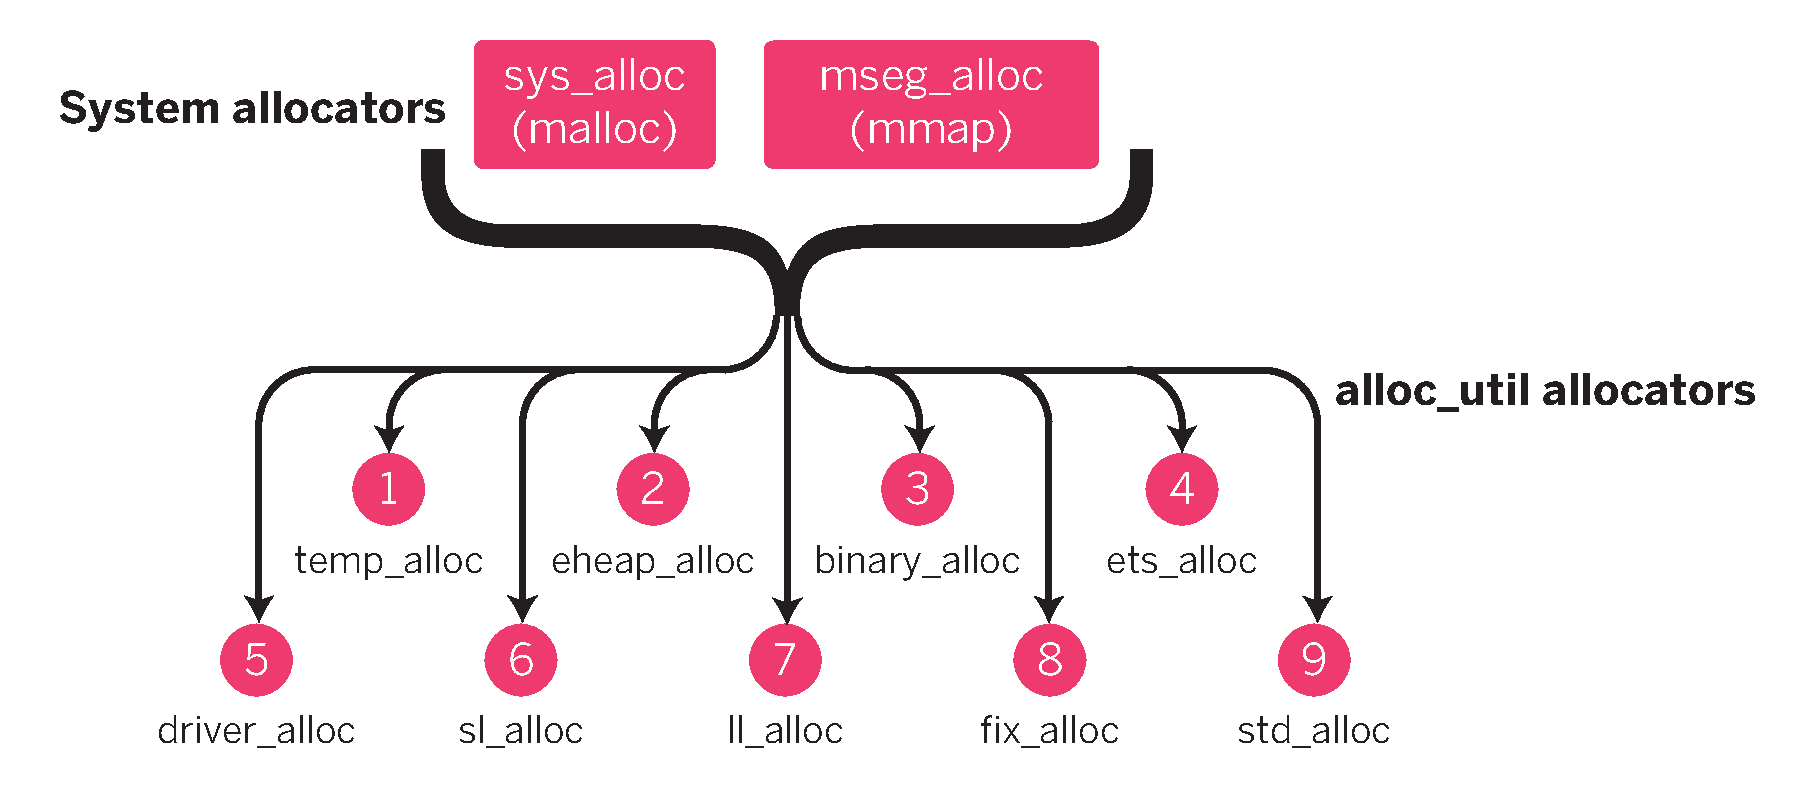
\includegraphics{memory-allocs.pdf}%
  \caption{Erlang's Memory allocators and their hierarchy. Not shown is the special \emph{super carrier}, optionally allowing to pre-allocate (and limit) all memory available to the Erlang VM since R16B03.}%
   \label{fig:allocators}
\end{figure}

\begin{enumerate*}
    \item \term{temp\_alloc}: does temporary allocations for short use cases (such as data living within a single C function call).
    \item \term{eheap\_alloc}: heap data, used for things such as the Erlang processes' heaps.
    \item \term{binary\_alloc}: the allocator used for reference counted binaries (what their 'global heap' is).
    \item \term{ets\_alloc}: ETS tables store their data in an isolated part of memory that isn't garbage collected, but allocated and deallocated as long as terms are being stored in tables.
    \item \term{driver\_alloc}: used to store driver data in particular, which doesn't keep drivers that generate Erlang terms from using other allocators. The driver data allocated here contains locks/mutexes, options, Erlang ports, etc.
    \item \term{sl\_alloc}: short-lived memory blocks will be stored there, and include items such as some of the VM's scheduling information or small buffers used for some data types' handling.
    \item \term{ll\_alloc}: long-lived allocations will be in there. Examples include Erlang code itself and the atom table, which stay there.
    \item \term{fix\_alloc}: allocator used for frequently used fixed-size blocks of memory. One example of data used there is the internal processes' C struct, used internally by the VM.
    \item \term{std\_alloc}: catch-all allocator for whatever didn't fit the previous categories. The process registry for named process is there.
\end{enumerate*}

By default, there will be one instance of each allocator per scheduler (and you should have one scheduler per core), plus one instance to be used by linked-in drivers using async threads. This ends up giving you a structure a bit like in Figure \ref{fig:allocators}, but split it in \var{N} parts at each leaf.

Each of these sub-allocators will request memory from \term{mseg\_alloc} and \term{sys\_alloc} depending on the use case, and in two possible ways. The first way is to act as a multiblock carrier (\term{mbcs}), which will fetch chunks of memory that will be used for many Erlang terms at once. For each \term{mbc}, the VM will set aside a given amount of memory (about 8MB by default in our case, which can be configured by tweaking VM options), and each term allocated will be free to go look into the many multiblock carriers to find some decent space in which to reside.

Whenever the item to be allocated is greater than the single block carrier threshold (\term{sbct})\footnote{\href{http://erlang.org/doc/man/erts\_alloc.html\#M\_sbct}{http://erlang.org/doc/man/erts\_alloc.html\#M\_sbct}}, the allocator switches this allocation into a single block carrier (\term{sbcs}). A single block carrier will request memory directly from \term{mseg\_alloc} for the first \term{mmsbc}\footnote{\href{http://erlang.org/doc/man/erts\_alloc.html\#M\_mmsbc}{http://erlang.org/doc/man/erts\_alloc.html\#M\_mmsbc}} entries, and then switch over to \term{sys\_alloc} and store the term there until it's deallocated.

So looking at something such as the binary allocator, we may end up with something similar to Figure \ref{fig:allocation-1-normal}

\begin{figure}
  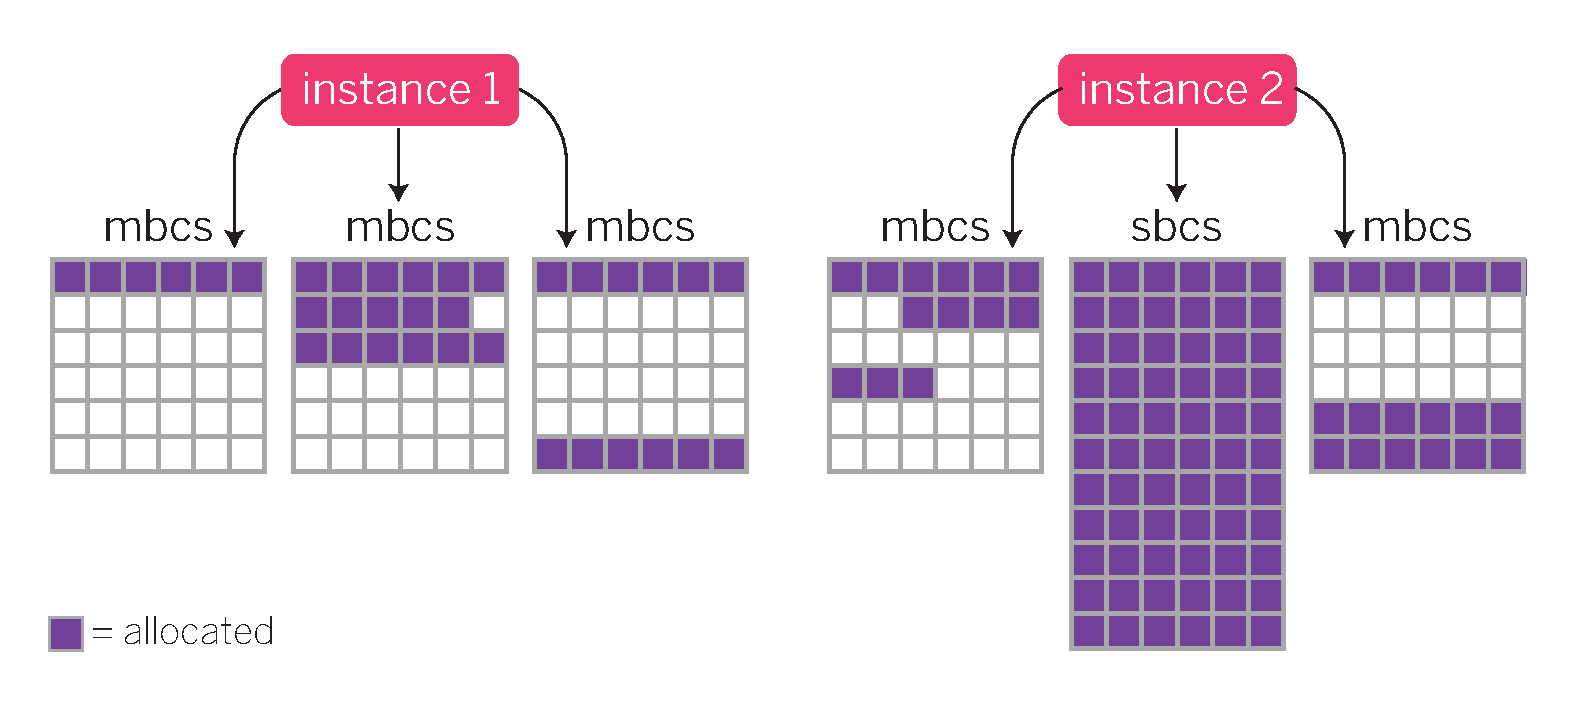
\includegraphics{allocation-1-normal.pdf}%
  \caption{Example memory allocated in a specific sub-allocator}%
   \label{fig:allocation-1-normal}
\end{figure}
\FloatBarrier

Whenever a multiblock carrier (or the first \term{mmsbc}\footnote{\href{http://erlang.org/doc/man/erts\_alloc.html\#M\_mmsbc}{http://erlang.org/doc/man/erts\_alloc.html\#M\_mmsbc}} single block carriers) can be reclaimed, \term{mseg\_alloc} will try to keep it in memory for a while so that the next allocation spike that hits your VM can use pre-allocated memory rather than needing to ask the system for more each time.

You then need to know the different memory allocation strategies of the Erlang virtual machine:

\begin{enumerate*}
    \item Best fit (\term{bf})
    \item Address order best fit (\term{aobf})
    \item Address order first fit (\term{aoff})
    \item Address order first fit carrier best fit (\term{aoffcbf})
    \item Address order first fit carrier address order best fit (\term{aoffcaobf})
    \item Good fit (\term{gf})
    \item A fit (\term{af})
\end{enumerate*}

Each of these strategies can be configured individually for each \term{alloc\_util} allocator\footnote{\href{http://erlang.org/doc/man/erts\_alloc.html\#M\_as}{http://erlang.org/doc/man/erts\_alloc.html\#M\_as}}

\begin{figure}
  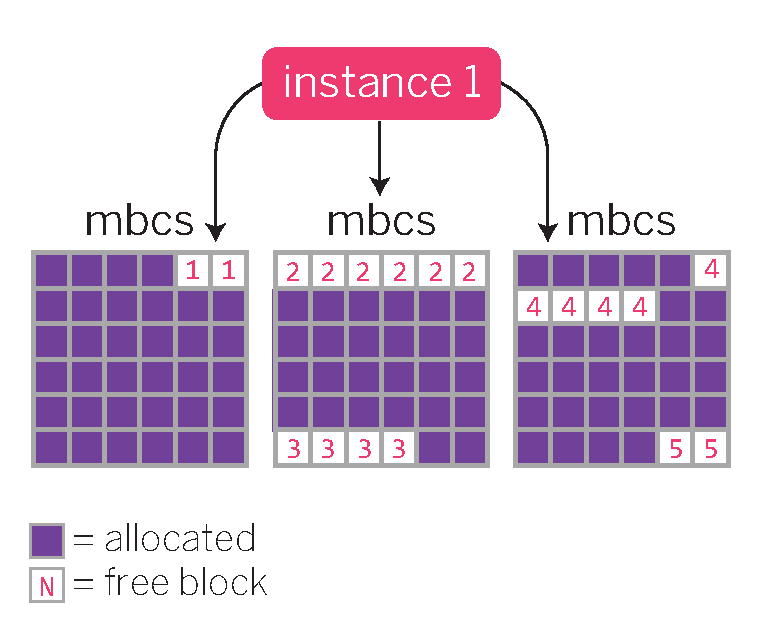
\includegraphics[max height=7cm]{allocation-strategy-1.pdf}%
  \centering%
  \caption{Example memory allocated in a specific sub-allocator}%
   \label{fig:allocation-strategy-1}
\end{figure}
\FloatBarrier

For \emph{best fit} (\term{bf}), the VM builds a balanced binary tree of all the free blocks' sizes, and will try to find the smallest one that will accommodate the piece of data and allocate it there. In Figure \ref{fig:allocation-strategy-1}, having a piece of data that requires three blocks would likely end in area 3.

\emph{Address order best fit} (\term{aobf}) will work similarly, but the tree instead is based on the addresses of the blocks. So the VM will look for the smallest block available that can accommodate the data, but if many of the same size exist, it will favor picking one that has a lower address. If I have a piece of data that requires three blocks, I'll still likely end up in area 3, but if I need two blocks, this strategy will favor the first \term{mbcs} in Figure \ref{fig:allocation-strategy-1} with area 1 (instead of area 5). This could make the VM have a tendency to favor the same carriers for many allocations.

\emph{Address order first fit} (\term{aoff}) will favor the address order for its search, and as soon as a block fits, \term{aoff} uses it. Where \term{aobf} and bf would both have picked area 3 to allocate four blocks in Figure \ref{fig:allocation-strategy-1}, this one will get area 2 as a first priority given its address is lowest. In Figure \ref{fig:allocation-strategy-2}, if we were to allocate four blocks, we'd favor block 1 to block 3 because its address is lower, whereas \term{bf} would have picked either 3 or 4, and \term{aobf} would have picked 3.

\begin{figure}
  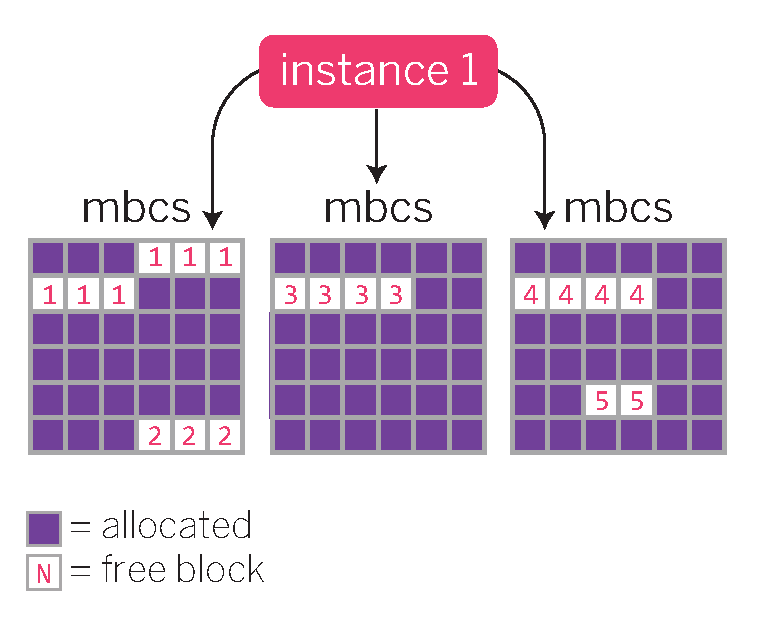
\includegraphics[max height=7cm]{allocation-strategy-2.pdf}%
  \centering%
  \caption{Example memory allocated in a specific sub-allocator}%
   \label{fig:allocation-strategy-2}
\end{figure}
\FloatBarrier

\emph{Address order first fit carrier best fit} (\term{aoffcbf}) is a strategy that will first favor a carrier that can accommodate the size and then look for the best fit within that one. So if we were to allocate two blocks in Figure \ref{fig:allocation-strategy-2}, \term{bf} and \term{aobf} would both favor block 5, \term{aoff} would pick block 1. \term{aoffcbf} would pick area 2, because the first \term{mbcs} can accommodate it fine, and area 2 fits it better than area 1.

\emph{Address order first fit carrier address order best fit} (\term{aoffcaobf}) will be similar to \term{aoffcbf}, but if multiple areas within a carrier have the same size, it will favor the one with the smallest address between the two rather than leaving it unspecified.

\emph{Good fit} (\term{gf}) is a different kind of allocator; it will try to work like best fit (\term{bf}), but will only search for a limited amount of time. If it doesn't find a perfect fit there and then, it will pick the best one encountered so far. The value is configurable through the \term{mbsd}\footnote{\href{http://www.erlang.org/doc/man/erts\_alloc.html\#M\_mbsd}{http://www.erlang.org/doc/man/erts\_alloc.html\#M\_mbsd}} VM argument.

\emph{A fit} (\term{af}), finally, is an allocator behaviour for temporary data that looks for a single existing memory block, and if the data can fit, \term{af} uses it. If the data can't fit, \term{af} allocates a new one.

Each of these strategies can be applied individually to every kind of allocator, so that the heap allocator and the binary allocator do not necessarily share the same strategy.

Finally, starting with Erlang version 17.0, each \term{alloc\_util} allocator on each scheduler has what is called a \emph{\term{mbcs} pool}. The \term{mbcs} pool is a feature used to fight against memory fragmentation on the VM. When an allocator gets to have one of its multiblock carriers become mostly empty,\footnote{The threshold is configurable through \href{http://www.erlang.org/doc/man/erts\_alloc.html\#M\_acul}{http://www.erlang.org/doc/man/erts\_alloc.html\#M\_acul}} the carrier becomes \emph{abandoned}. 

This abandoned carrier will stop being used for new allocations, until new multiblock carriers start being required. When this happens, the carrier will be fetched from the \term{mbcs} pool. This can be done across multiple \term{alloc\_util} allocators of the same type across schedulers. This allows to cache mostly-empty carriers without forcing deallocation of their memory.\footnote{in cases this consumes too much memory, the feature can be disabled with the options \term{+MBacul 0}.} It also enables the migration of memory blocks across schedulers when they contain little data, according to their needs.

\subsubsection{The Process Level}
\label{subsec:memory-process-level}

On a smaller scale, for each Erlang process, the layout still is a bit different. It basically has this piece of memory that can be imagine as one box:

\begin{VerbatimText}
[                  ]
\end{VerbatimText}

On one end you have the heap, and on the other, you have the stack:

\begin{VerbatimText}
[heap |     | stack]
\end{VerbatimText}

In practice there's more data (you have an old heap and a new heap, for generational GC, and also a virtual binary heap, to account for the space of reference-counted binaries on a specific sub-allocator not used by the process — \term{binary\_alloc} vs. \term{eheap\_alloc}):

\begin{VerbatimText}
[heap   ||    stack]
\end{VerbatimText}

The space is allocated more and more up until either the stack or the heap can't fit in anymore. This triggers a minor GC. The minor GC moves the data that can be kept into the old heap, GCs the rest, may end up reallocating for more space.

After a given number of minor GCs and/or reallocations, a full-sweep GC is performed, which inspects both the new and old heaps, frees up more space, and so on. When a process dies, both the stack and heap are taken out at once. reference-counted binaries are decreased, and if the counter is at 0, they vanish.

When that happens, over 80\% of the time, the only thing that happens is that the memory is marked as available in the sub-allocator and can be taken back by new processes or other ones that may need to be resized. Only after having this memory unused — and the multiblock carrier unused also — is it returned to \term{mseg\_alloc} or \term{sys\_alloc}, which may or may not keep it for a while longer.

\subsection{Fixing Memory Fragmentation with a Different Allocation Strategy}

Tweaking your VM's options for memory allocation may help.

You will likely need to have a good understanding of what your type of memory load and usage is, and be ready to do a lot of in-depth testing. The \module{recon\_alloc} module contains a few helper functions to provide guidance, and the module's documentation\footnote{\href{http://ferd.github.io/recon/recon\_alloc.html}{http://ferd.github.io/recon/recon\_alloc.html}} should be read at this point.

You will need to figure out what the average data size is, the frequency of allocation and deallocation, whether the data fits in \term{mbcs} or \term{sbcs},  and you will then need to try playing with a bunch of the options mentioned in \module{recon\_alloc}, try the different strategies, deploy them, and see if things improve or if they impact times negatively.

This is a very long process for which there is no shortcut, and if issues happen only every few months per node, you may be in for the long haul. 


\section{Exercises}

\subsection{Review Questions}

\begin{enumerate}
	\item Name some of the common sources of leaks in Erlang programs.
	\item What are the two main types of binaries in Erlang?
	\item What could be to blame if no specific data type seems to be the source of a leak?
	\item If you find the node died with a process having a lot of memory, what could you do to find out which one it was?
	\item How could code itself cause a leak?
	\item How can you find out if garbage collections are taking too long to run?
\end{enumerate}

\subsection{Open-ended Questions}

\begin{enumerate}
	\item  How could you verify if a leak is caused by forgetting to kill processes, or by processes using too much memory on their own?
	\item A process opens a 150MB log file in binary mode to go extract a piece of information from it, and then stores that information in an ETS table. After figuring out you have a binary memory leak, what should be done to minimize binary memory usage on the node?
	\item What could you use to find out if ETS tables are growing too fast?
	\item What steps should you go through to find out that a node is likely suffering from fragmentation? How could you disprove the idea that is could be due to a NIF or driver leaking memory?
	\item How could you find out if a process with a large mailbox (from reading \term{message\_queue\_len}) seems to be leaking data from there, or never handling new messages?
	\item A process with a large memory footprint seems to be rarely running garbage collections. What could explain this?
	\item When should you alter the allocation strategies on your nodes? Should you prefer to tweak this, or the way you wrote code?
\end{enumerate}

\subsection{Hands-On}

\begin{enumerate}
	\item Using any system you know or have to maintain in Erlang (including toy systems), can you figure out if there are any binary memory leaks on there?
\end{enumerate}
	
%%%
%%%
%%%

%%% Cognitive
%%
%% These should be done after reading the standard documentation on crash dumps referenced by the text.
%%
%% Knowledge: recall facts, terms, basic concepts
%% 
%% - What are the two main ways to find about a memory leak?
%% - What are good questions to ask about the node if you suspect a leak?
%% - Name some of the common sources of leaks in Erlang programs.
%% - What are the two main types of binaries in Erlang?
%% - What could be to blame if no specific data type seems guilty of a leak?
%% - Can Erlang's memory allocation schemes be modified or are they unchangeable without patches?
%%
%% Comprehension: organizing, comparing, translating, interpreting, giving descriptions, and stating the main ideas
%%
%% - How could you verify if a leak is caused by forgetting to kill processes, or by processes using too much memory on their own?
%% - What could cause the atom table to grow infinitely?
%% - How could code itself cause a leak?
%% - How can you find out if garbage collections are taking too long to run?
%%
%% Application: Solve problems in new situations by applying acquired knowledge, facts, techniques and rules in a different way
%%
%% - Using any system you know or have to maintain in Erlang (including toy systems), can you figure out if there are any binary memory leaks on there?
%% - A process opens a 150MB log file in binary mode to go extract a piece of information from it, and then stores that information in an ETS table. After figuring out you have a binary memory leak, what should be done to minimize binary memory usage on the node?
%% - What could you use to find out if ETS tables are growing too fast?
%%
%% Analysis: break down info, make inferences, find evidence
%%
%% - What steps should you go through to find out that a node is likely suffering from fragmentation? How could you disprove the idea that is could be due to a NIF or driver leaking memory?
%%
%% Synthesis: Compile information together in a different way by combining elements in a new pattern or proposing alternative solutions
%%
%% - How could you find out if a process with a large mailbox (from reading 'message_queue_len') seems to be leaking data from there, or never handling new messages?
%% - A process with a large memory footprint seems to be rarely running garbage collections. What could explain this?
%%
%% Evaluation: Present and defend opinions by making judgments about information
%%
%% - When should you alter the allocation strategies on your nodes? Should you prefer to tweak this, or the way you wrote code?
%% 

%%%
%%%
%%%

\chapter{CPU and Scheduler Hogs}
\label{chap:cpu-hogs}

While memory leaks tend to absolutely kill your system, CPU exhaustion tends to act like a bottleneck and limits the maximal work you can get out of a node. Erlang developers will have a tendency to scale horizontally when they face such issues. It is often an easy enough job to scale out the more basic pieces of code out there. Only centralized global state (process registries, ETS tables, and so on) usually need to be modified.\footnote{Usually this takes the form of sharding or finding a state-replication scheme that's suitable, and little more. It's still a decent piece of work, but nothing compared to finding out most of your program's semantics aren't applicable to distributed systems given Erlang usually forces your hand there in the first place.} Still, if you want to optimize locally before scaling out at first, you need to be able to find your CPU and scheduler hogs.

It is generally difficult to properly analyze the CPU usage of an Erlang node to pin problems to a specific piece of code. With everything concurrent and in a virtual machine, there is no guarantee you will find out if a specific process, driver, your own Erlang code, NIFs you may have installed, or some third-party library is eating up all your processing power.

The existing approaches are often limited to profiling and reduction-counting if it's in your code, and to monitoring the scheduler's work if it might be anywhere else (but also your code).

\section{Profiling and Reduction Counts}
\label{sec:cpu-profiling}

To pin issues to specific pieces of Erlang code, as mentioned earlier, there are two main approaches. One will be to do the old standard profiling routine, likely using one of the following applications:\footnote{All of these profilers work using Erlang tracing functionality with almost no restraint. They will have an impact on the run-time performance of the application, and shouldn't be used in production.}

\begin{itemize*}
	\item \otpapp{eprof},\footnote{\href{http://www.erlang.org/doc/man/eprof.html}{http://www.erlang.org/doc/man/eprof.html}} the oldest Erlang profiler around. It will give general percentage values and will mostly report in terms of time taken.
	\item \otpapp{fprof},\footnote{\href{http://www.erlang.org/doc/man/fprof.html}{http://www.erlang.org/doc/man/fprof.html}} a more powerful replacement of eprof. It will support full concurrency and generate in-depth reports. In fact, the reports are so deep that they are usually considered opaque and hard to read. 
	\item \otpapp{eflame},\footnote{\href{https://github.com/proger/eflame}{https://github.com/proger/eflame}} the newest kid on the block. It generates flame graphs to show deep call sequences and hot-spots in usage on a given piece of code. It allows to quickly find issues with a single look at the final result.
\end{itemize*}

Which will be left to the reader to do through reading each of these application's documentation.

The other approach will be to run \function{recon:proc\_window/3} as introduced in Subsection \ref{subsec:digging-procs}:

\begin{VerbatimEshell}
1> recon:proc_window(reductions, 3, 500).
[{<0.46.0>,51728,
  [{current_function,{queue,in,2}},
   {initial_call,{erlang,apply,2}}]},
 {<0.49.0>,5728,
  [{current_function,{dict,new,0}},
   {initial_call,{erlang,apply,2}}]},
 {<0.43.0>,650,
  [{current_function,{timer,sleep,1}},
   {initial_call,{erlang,apply,2}}]}]
\end{VerbatimEshell}

The reduction count has a direct link to function calls in Erlang, and a high count is usually the synonym of a high amount of CPU usage. 

What's interesting with this function is to try it while a system is already rather busy,\footnote{See Subsection \ref{subsec:global-cpu}} with a relatively short interval. Repeat it many times, and you should hopefully see a pattern emerge where the same processes (or the same \emph{kind} of processes) tend to always come up on top.

Using the code locations\footnote{Call \expression{recon:info(PidTerm, location)} or \expression{process\_info(Pid, current\_stacktrace)} to get this information.} and current functions being run, you should be able to identify what kind of code hogs all your schedulers.

\section{System Monitors}
\label{sec:cpu-system-monitors}

If nothing seems to stand out through either profiling or checking reduction counts, it's possible some of your work ends up being done by NIFs, garbage collections, and so on. These kinds of work may not always increment their reductions count correctly, so they won't show up with the previous methods, only through long run times.

To find about such cases, the best way around is to use \function{erlang:system\_monitor/2}, and look for \term{long\_gc} and \term{long\_schedule}. The former will show whenever garbage collection ends up doing a lot of work (it takes time!), and the latter will likely catch issues with busy processes, either through NIFs or some other means, that end up making them hard to de-schedule.\footnote{long garbage collections count towards scheduling time. It is very possible that a lot of your long schedules will be tied to garbage collections depending on your system.}

We've seen how to set such a system monitor In Garbage Collection in \ref{subsubsec:leak-gc}, but here's a different pattern\footnote{If you're on 17.0 or newer versions, the shell functions can be made recursive far more simply by using their named form, but to have the widest compatibility possible with older versions of Erlang, I've let them as is.} I've used before to catch long-running items:

\begin{VerbatimEshell}
1> F = fun(F) ->
    receive
        {monitor, Pid, long_schedule, Info} ->
            io:format("monitor=long_schedule pid=~p info=~p~n", [Pid, Info]);
        {monitor, Pid, long_gc, Info} -> 
            io:format("monitor=long_gc pid=~p info=~p~n", [Pid, Info])
    end,
    F(F)
end.
2> Setup = fun(Delay) -> fun() -> 
     register(temp_sys_monitor, self()),
     erlang:system_monitor(self(), [{long_schedule, Delay}, {long_gc, Delay}]),
     F(F)
end end.
3> spawn_link(Setup(1000)).
<0.1293.0>
monitor=long_schedule pid=<0.54.0> info=[{timeout,1102},
                                         {in,{some_module,some_function,3}},
                                         {out,{some_module,some_function,3}}]
\end{VerbatimEshell}

Be sure to set the \term{long\_schedule} and \term{long\_gc} values to large-ish values that might be reasonable to you. In this example, they're set to 1000 milliseconds. You can either kill the monitor by calling \expression{exit(whereis(temp\_sys\_monitor), kill)} (which will in turn kill the shell because it's linked), or just disconnect from the node (which will kill the process because it's linked to the shell.)

This kind of code and monitoring can be moved to its own module where it reports to a long-term logging storage, and can be used as a canary for performance degradation or overload detection.

\subsection{Suspended Ports}
\label{subsec:port-system-monitors}

An interesting part of system monitors that didn't fit anywhere but may have to do with scheduling is regarding ports. When a process sends too many message to a port and the port's internal queue gets full, the Erlang schedulers will forcibly de-schedule the sender until space is freed. This may end up surprising a few users who didn't expect that implicit back-pressure from the VM.

This kind of event can be monitored by passing in the atom \term{busy\_port} to the system monitor. Specifically for clustered nodes, the atom \term{busy\_dist\_port} can be used to find when a local process gets de-scheduled when contacting a process on a remote node whose inter-node communication was handled by a busy port.

If you find out you're having problems with these, try replacing your sending functions where in critical paths with \function{erlang:port\_command(Port, Data, [nosuspend])} for ports, and \function{erlang:send(Pid, Msg, [nosuspend])} for messages to distributed processes. They will then tell you when the message could not be sent and you would therefore have been descheduled.


\section{Exercises}

\subsection{Review Questions}

\begin{enumerate}
	\item What are the two main approaches to pin issues about CPU usages?
	\item Name some of the profiling tools available. What approaches are preferable for production use? Why?
	\item Why can long scheduling monitors be useful to find CPU or scheduler over-consumption?

\end{enumerate}

\subsection{Open-ended Questions}

\begin{enumerate}
	\item If you find that a process doing very little work with reductions ends up being scheduled for long periods of time, what can you guess about it or the code it runs?
	\item Can you set up a system monitor and then trigger it with regular Erlang code? Can you use it to find out for how long processes seem to be scheduled on average? You may need to manually start random processes from the shell that are more aggressive in their work than those provided by the existing system.
\end{enumerate}

%%%
%%%
%%%

%%% Cognitive
%%
%% These should be done after reading the standard documentation on crash dumps referenced by the text.
%%
%% Knowledge: recall facts, terms, basic concepts
%% 
%% - What are the two main approaches to pin issues about CPU usages?
%% - Name some of the profiling tools available
%%
%% Comprehension: organizing, comparing, translating, interpreting, giving descriptions, and stating the main ideas
%%
%% - What approaches are preferable for production use? Why?
%% - Why can long scheduling monitors be useful to find CPU or scheduler over-consumption?
%%
%% Application: Solve problems in new situations by applying acquired knowledge, facts, techniques and rules in a different way
%%
%% - Can you set up a system monitor and then trigger it with regular Erlang code? Can you use it to find out for how long processes seem to be scheduled on average?
%%
%% Analysis: break down info, make inferences, find evidence
%%
%% - If you find that a process doing very little work with reductions ends up being scheduled for long periods of time, what can you guess about it or the code it runs?
%%
%% Synthesis: Compile information together in a different way by combining elements in a new pattern or proposing alternative solutions
%%
%% - A set of heavily loaded processes appear to be working fine most of the time, but eventually have their queues build up and get bogged down more and more. You suspect this might be because the process is overworked. What would you test to find the source of the issue?
%% - No process particularly stands out as being using a lot of CPU on the node. What can you do to determine whether one piece of code run many times is using too much CPU or whether the node is just purely overloaded?
%%
%% Evaluation: Present and defend opinions by making judgments about information
%%
%% - Try any of the profiling tools on any given code base. Which one do you prefer? Why?
%% 

%%%
%%%
%%%

\chapter{Tracing}
\label{chap:tracing}

One of the lesser known and absolutely under-used features of Erlang and the BEAM virtual machine is just about how much tracing you can do on there.

Forget your debuggers, their use is too limited.\footnote{One common issue with debuggers that let you insert break points and step through a program is that they are incompatible with many Erlang programs: put a break point in one process and the ones around keep going. In practice, this turns debugging into a very limited activity because as soon as a process needs to interact with the one you're debugging, its calls start timing out and crashing, possibly taking down the entire node with it. Tracing, on the other hand, doesn't interfere with program execution, but still gives you all the data you need.} Tracing makes sense in Erlang at all steps of your system's life cycle, whether it's for development or for diagnosing a running production system. 

There are a few options available to trace Erlang programs:

\begin{itemize}
	\item \module{sys}\footnote{\href{http://www.erlang.org/doc/man/sys.html}{http://www.erlang.org/doc/man/sys.html}} comes standard with OTP and allows to set custom tracing functions, log all kinds of events, and so on. It's generally complete and fine to use for development. It suffers a bit in production because it doesn't redirect IO to remote shells, and doesn't have rate-limiting capabilities for trace messages. It is still recommended to read the documentation for the module.
	
	\item \otpapp{dbg}\footnote{\href{http://www.erlang.org/doc/man/dbg.html}{http://www.erlang.org/doc/man/dbg.html}} also comes standard with Erlang/OTP. Its interface is a bit clunky in terms of usability, but it's entirely good enough to do what you need. The problem with it is that you \emph{have to know what you're doing}, because \otpapp{dbg} can log absolutely everything on the node and kill one in under two seconds.
	
	\item \emph{tracing BIFs} are available as part of the \module{erlang} module. They're mostly the raw blocks used by all the applications mentioned in this list, but their lower level of abstraction makes them rather difficult to use.
	
	\item \otpapp{redbug}\footnote{\href{https://github.com/massemanet/eper/blob/master/doc/redbug.txt}{https://github.com/massemanet/eper/blob/master/doc/redbug.txt}} is a production-safe tracing library, part of the \otpapp{eper}\footnote{\href{https://github.com/massemanet/eper}{https://github.com/massemanet/eper}} suite. It has an internal rate-limiter, and a nice usable interface. To use it, you must however be willing to add in all of \otpapp{eper}'s dependencies. The toolkit is fairly comprehensive and can be a very interesting install.
	
	\item \module{recon\_trace}\footnote{\href{http://ferd.github.io/recon/recon\_trace.html}{http://ferd.github.io/recon/recon\_trace.html}} is \otpapp{recon}'s take on tracing. The objective was to allow the same levels of safety as with \otpapp{redbug}, but without the dependencies. The interface is different, and the rate-limiting options aren't entirely identical. It can also only trace function calls, and not messages.\footnote{Messages may be supported in future iterations of the library. In practice, the author hasn't found the need when using OTP, given behaviours and matching on specific arguments allows to get something roughly equivalent.}
\end{itemize}

This chapter will focus on tracing with \module{recon\_trace}, but the terminology and the concepts used mostly carry over to any other Erlang tracing tool that can be used.

\section{Tracing Principles}
\label{sec:tracing-princples}

The Erlang Trace BIFs allow to trace any Erlang code at all\footnote{In cases where processes contain sensitive information, data can be forced to be kept private by calling \expression{process\_flag(sensitive, true)}}. They work in two parts: \emph{pid specifications}, and \emph{trace patterns}.

Pid specifications lets the user decide which processes to target. They can be specific pids, \expression{all} pids, \expression{existing} pids, or \expression{new} pids (those not spawned at the time of the function call).

The trace patterns represent functions. Functions can be specified in two parts: specifying the modules, functions, and arity, and then with Erlang match specifications\footnote{\href{http://www.erlang.org/doc/apps/erts/match\_spec.html}{http://www.erlang.org/doc/apps/erts/match\_spec.html}} to add constraints to arguments.

What defines whether a specific function call gets traced or not is the intersection of both, as seen in Figure~\ref{fig:tracing-venn}.

\begin{figure}
  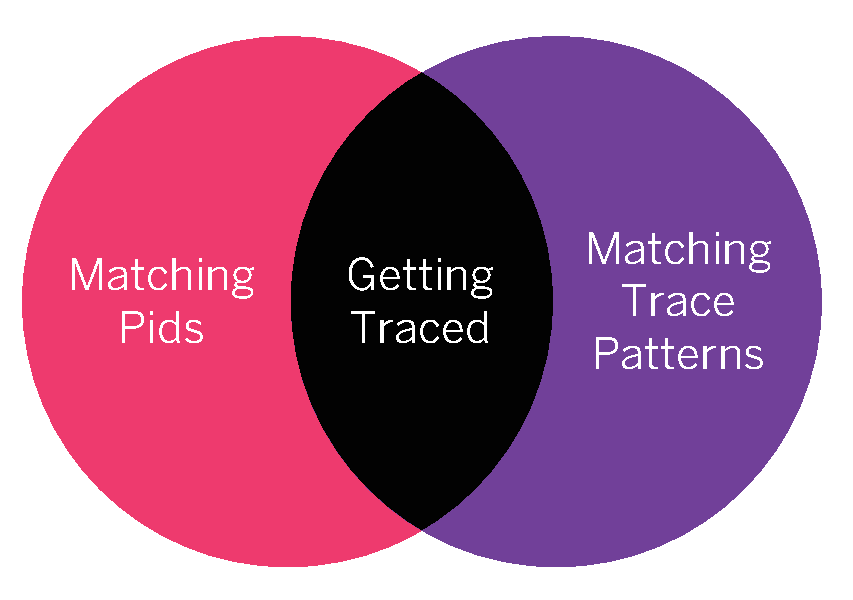
\includegraphics[max height=7cm]{tracing-venn.pdf}%
  \centering%
  \caption{What gets traced is the result of the intersection between the matching pids and the matching trace patterns}%
   \label{fig:tracing-venn}
\end{figure}

If either the pid specification excludes a process or a trace pattern excludes a given call, no trace will be received.

Tools like \otpapp{dbg} (and trace BIFs) force you to work with this Venn diagram in mind. You specify sets of matching pids and sets of trace patterns independently, and whatever happens to be at the intersection of both sets gets to be displayed.

Tools like \otpapp{redbug} and \module{recon\_trace}, on the other hand, abstract this away.
\FloatBarrier

\section{Tracing with Recon}

Recon, by default, will match all processes. This will often be good enough for a lot of debugging cases. The interesting part you'll want to play with most of the time is specification of trace patterns. Recon support a few basic ways to declare them. 

The most basic form is \expression{\{Mod, Fun, Arity\}}, where a literal module, function name, arity (number) or wildcards (\expression{'\_'}). Recon will forbid forms that match too widely on everything (such as \expression{\{'\_','\_','\_'\}}), as they could be plain dangerous to run in production.

A fancier form will be to replace the arity by a function to match on lists of arguments. The function is limited to those usable by match specifications similar to what is available in ETS\footnote{\href{http://www.erlang.org/doc/man/ets.html\#fun2ms-1}{http://www.erlang.org/doc/man/ets.html\#fun2ms-1}}. Finally, multiple patterns can be put into a list to broaden the matching scope.

It will also be possible to rate limit based on two manners: a static count, or a number of matches per time interval.

Rather than going more in details, here's list of examples and how to trace for them.

\begin{VerbatimErl}
%% All calls from the queue module, with 10 calls printed at most:
recon_trace:calls({queue, '_', '_'}, 10)

%% All calls to lists:seq(A,B), with 100 calls printed at most:
recon_trace:calls({lists, seq, 2}, 100)

%% All calls to lists:seq(A,B), with 100 calls per second at most:
recon_trace:calls({lists, seq, 2}, {100, 1000})

%% All calls to lists:seq(A,B,2) (all sequences increasing by two) with 100 calls
%% at most:
recon_trace:calls({lists, seq, fun([_,_,2]) -> ok end}, 100)

%% All calls to iolist_to_binary/1 made with a binary as an argument already
%% (a kind of tracking for useless conversions):
recon_trace:calls({erlang, iolist_to_binary,
                   fun([X]) when is_binary(X) -> ok end},
                  10)

%% Calls to the queue module only in a given process Pid, at a rate of 50 per
%% second at most:
recon_trace:calls({queue, '_', '_'}, {50,1000}, [{pid, Pid}])

%% Print the traces with the function arity instead of literal arguments:
recon_trace:calls(TSpec, Max, [{args, arity}])

%% Matching the filter/2 functions of both dict and lists modules, across new
%% processes only:
recon_trace:calls([{dict,filter,2},{lists,filter,2}], 10, [{pid, new]})

%% Tracing the handle_call/3 functions of a given module for all new processes,
%% and those of an existing one registered with gproc:
recon_trace:calls({Mod,handle_call,3}, {1,100}, [{pid, [{via, gproc, Name}, new]}

%% Show the result of a given function call, the important bit being the
%% return_trace() call or the {return_trace} match spec value.
recon_trace:calls({Mod,Fun,fun(_) -> return_trace() end}, Max, Opts)
recon_trace:calls({Mod,Fun,[{'_', [], [{return_trace}]}]}, Max, Opts)

\end{VerbatimErl}

Each call made will override the previous one, and all calls can be cancelled with \function{recon\_trace:clear/0}.

There's a few more combination possible, with more options:

\begin{description}
	\item[\expression{\{pid, PidSpec\}}] \hfill
	
		Which processes to trace. Valid options is any of \term{all}, \term{new}, \term{existing}, or a process descriptor (\expression{\{A,B,C\}}, \expression{"<A.B.C>"}, an atom representing a name, \expression{\{global, Name\}}, \expression{\{via, Registrar, Name\}}, or a pid). It's also possible to specify more than one by putting them in a list.
		
	\item[\expression{\{timestamp, formatter | trace\}}] \hfill
	
		By default, the formatter process adds timestamps to messages received. If accurate timestamps are required, it's possible to force the usage of timestamps within trace messages by adding the option \expression{\{timestamp, trace\}}.
		
	\item[\expression{\{args, arity | args\}}] \hfill
	
		Whether to print the arity in function calls or their (by default) literal representation.
		
 	\item[\expression{\{scope, global | local\}}] \hfill
	
		By default, only 'global' (fully qualified function calls) are traced, not calls made internally. To force tracing of local calls, pass in \expression{\{scope, local\}}. This is useful whenever you want to track the changes of code in a process that isn't called with \expression{Module:Fun(Args)}, but just \expression{Fun(Args)}.
\end{description}

With these options, the multiple ways to pattern match on specific calls for specific functions and whatnot, a lot of development and production issues can more quickly be diagnosed. If the idea ever comes to say "hm, maybe I should add more logging there to see what could cause that funny behaviour", tracing can usually be a very fast shortcut to get the data you need without deploying any code or altering its readability.


\section{Example Sessions}

First let's trace the queue:new functions in any process:

\begin{VerbatimEshell}
1> recon_trace:calls({queue, new, '_'}, 1).
1
13:14:34.086078 <0.44.0> queue:new()
Recon tracer rate limit tripped.
\end{VerbatimEshell}

The limit was set to 1 trace message at most, and recon let us know when that limit was reached.

Let's instead look for all the \function{queue:in/2} calls, to see what it is we're inserting in queues:

\begin{VerbatimEshell}
2> recon_trace:calls({queue, in, 2}, 1).
1
13:14:55.365157 <0.44.0> queue:in(a, {[],[]})
Recon tracer rate limit tripped.
\end{VerbatimEshell}

In order to see the content we want, we should change the trace patterns to use a fun that matches on all arguments in a list (\term{\_}) and returns \expression{return\_trace()}. This last part will generate a second trace for each call that includes the return value:

\begin{VerbatimEshell}
3> recon_trace:calls({queue, in, fun(_) -> return_trace() end}, 3).
1

13:15:27.655132 <0.44.0> queue:in(a, {[],[]})

13:15:27.655467 <0.44.0> queue:in/2 --> {[a],[]}

13:15:27.757921 <0.44.0> queue:in(a, {[],[]})
Recon tracer rate limit tripped.
\end{VerbatimEshell}

Matching on argument lists can be done in a more complex manner:

\begin{VerbatimEshell}
4> recon_trace:calls(
4>   {queue, '_',
4>    fun([A,_]) when is_list(A); is_integer(A) andalso A > 1 ->
4>        return_trace()
4>    end},
4>   {10,100}
4> ).
32

13:24:21.324309 <0.38.0> queue:in(3, {[],[]})

13:24:21.371473 <0.38.0> queue:in/2 --> {[3],[]}

13:25:14.694865 <0.53.0> queue:split(4, {[10,9,8,7],[1,2,3,4,5,6]})

13:25:14.695194 <0.53.0> queue:split/2 --> {{[4,3,2],[1]},{[10,9,8,7],[5,6]}}

5> recon_trace:clear().
ok
\end{VerbatimEshell}

Note that in the pattern above, no specific function (\expression{'\_'}) was matched against. Instead, the fun used restricted functions to those having two arguments, the first of which is either a list or an integer greater than 1.

Be aware that extremely broad patterns with lax rate-limitting (or very high absolute limits) may impact your node's stability in ways \module{recon\_trace} cannot easily help you with. Similarly, tracing extremely large amounts of function calls (all of them, or all of \module{io} for example) can be risky if more trace messages are generated than any process on the node could ever handle, despite the precautions taken by the library.

In doubt, start with the most restrictive tracing possible, with low limits, and progressively increase your scope.


\section{Exercises}

\subsection{Review Questions}

\begin{enumerate}
	\item Why is debugger use generally limited on Erlang?
	\item What are the options you can use to trace OTP processes?
	\item What determines whether a given set of functions or processes get traced?
	\item How can you stop tracing with \module{recon\_trace}? With other tools?
	\item How can you trace non-exported function calls?
\end{enumerate}

\subsection{Open-ended Questions}

\begin{enumerate}
	\item When would you want to move time stamping of traces to the VM's trace mechanisms directly? What would be a possible downside of doing this?	
	\item Imagine that traffic sent out of a node does so over SSL, over a multi-tenant system. However, due to wanting to validate data sent (following a customer complain), you need to be able to inspect what was seen clear text. Can you think up a plan to be able to snoop in the data sent to their end through the \module{ssl} socket, without snooping on the data sent to any other customer?
\end{enumerate}

\subsection{Hands-On}

Using the code at \href{https://github.com/ferd/recon\_demo}{https://github.com/ferd/recon\_demo} (these may require a decent understanding of the code there):

\begin{enumerate}
	\item Can chatty processes (\module{council\_member}) message themselves? (\emph{hint: can this work with registered names? Do you need to check the chattiest process and see if it messages itself?})
	\item Can you estimate the overall frequency at which messages are sent globally?
	\item Can you crash a node using any of the tracing tools? (\emph{hint: dbg makes it easier due to its greater flexibility})
\end{enumerate}


%%%
%%%
%%%

%%% Cognitive
%%
%% These should be done after reading the standard documentation on crash dumps referenced by the text.
%%
%% Knowledge: recall facts, terms, basic concepts
%% 
%% - Why is debugger use limited on Erlang?
%% - What are options you can use to trace OTP processes?
%%
%% Comprehension: organizing, comparing, translating, interpreting, giving descriptions, and stating the main ideas
%%
%% - What determines whether a given set of functions or processes get traced?
%% - How can you stop tracing with recon_trace?
%% - How can you trace non-exported function calls?
%%
%% Application: Solve problems in new situations by applying acquired knowledge, facts, techniques and rules in a different way
%%
%% Using https://github.com/ferd/recon_demo
%% - Can chatty processes message themselves? (can this work with registered names? Do I need to check the chattiest one and see if it messages itself?)
%% - Can you estimate the overall frequency at which messages are sent globally?
%% - Can you crash a node using any of the tracing tools? (hint: dbg makes it easier due to its flexibility)
%%
%% Analysis: break down info, make inferences, find evidence
%%
%% - When would you want to move time stamping of traces to the VM's trace mechanisms directly? What would be a possible downside of doing this?
%%
%% Synthesis: Compile information together in a different way by combining elements in a new pattern or proposing alternative solutions
%%
%% - Imagine that traffic sent out of a node does so over SSL, over a multi-tenant system. However, due to wanting to validate data sent (following a customer complain), you need to be able to inspect what was seen clear text. Can you think up a plan to be able to snoop in the data sent to their end through the 'ssl' socket, without snooping on the data sent to any other customer?
%%
%% Evaluation: Present and defend opinions by making judgments about information
%%
%% - Do you think tracing is more useful than debugging, even in development? If not, why?
%% 


%%%
%%% Tuning the VM: not a chapter yet.
%%%


%% locks!

%% you usually want the lmbcs to be at least a 5 times (if not more) bigger than the perc95

%% the binaries will still count as binary data if you move it to ets. It is only the pointer to the binary that moves from the heap to ets. (for binaries > 64 bytes)

%% Cache hits

%% Kernel Polling

%% 

\chapter{Conclusion}

There is no such thing as a conclusion, because maintaining and debugging software never ends. New bugs and confusing behaviours will keep popping up around the place all the time. There would probably be enough stuff out there to fill out dozens of  manuals like these, even when dealing with the cleanest of all systems.

Even the most solid bridges need to be repainted all the time in order avoid corrosion to the point of their collapse. Best of luck to you.

\end{document}  
